\documentclass{Format}
%Libraries
\usepackage{mhchem} % Paquete para escribir ecuaciones químicas
\usepackage{booktabs} % Paquete para mejorar la apariencia de las tablas
\usepackage{multicol}
\usepackage[numbers]{natbib} % Usa natbib para la gestión de citas
\usepackage{graphicx}
\usepackage{caption}
\usepackage{amsmath}
\usepackage{subcaption}
%usepackage[spanish]{babel}
\usepackage{float} 
\usepackage{enumitem}
\usepackage{algorithm}
\usepackage{algpseudocode}
\usepackage{tikz}
\usetikzlibrary{shapes.multipart}
\usepackage[dvipsnames]{xcolor}
\usepackage{xcolor}
\usepackage{mdframed}



% Title
\title{\LARGE[241030] Simulation of Turboprop Systems using Simulink: Development and Validation of Computational Mechanical Model}

% Authors
\author{
% Centrar los primeros tres nombres
\begin{tabular}{c}
\Large Sofia Valentina Delgado Pinzón\textsuperscript{a,c}, 
\Large Juan Pablo González Posada\textsuperscript{a,c}\\
\\
\Large Juan José Reyes Perilla\textsuperscript{a,c} \\
\
\Large Camilo Andres Bayona Roa\textsuperscript{b,c} \\
\end{tabular}
}


\begin{document}

\maketitle
\noindent\hrulefill
\begin{abstract}

The present work is the development of a computational tool in the software Simulink-Matlab \cite{SimulinkMathworks}, consisting of an aerothermodynamic model to simulate the behavior of a Turboprop engine under different flight conditions. The thermodynamic theory and \textit{Blade Element Momentum Theory} (BEMT) \cite{Winarto2004BEMT} is implemented for said model. In this sense, the software supports the maintenance, manufacturing, and energy reconversion of the Turboprop engine at a national level.

The computational tool provides outputs such as performance, behavior, and efficiency of the Turboprop engine, based on inputs such as the fuel implemented (conventional or alternative), air flow conditions, propeller geometry, aerodynamic characteristics of the blade profiles, and operating regimes of the engine. Thus, results demonstrate that the software supports informed decision-making in the aeronautical industry and will guide it towards the realistic implementation of preoperation computational simulations.

\end{abstract}
\begin{center}
\textbf{\textit{\fontsize{8}{10}\selectfont Keywords:}} \textit{\fontsize{8}{10}\selectfont BEMT, Aerothermodynamic, Turboprop, Simulink-Matlab and Computational Tool}
\end{center}

\noindent\hrulefill

% Main Content

\section{\bfseries\fontsize{10}{12}\selectfont Justification and Problem Statement}\label{sec:intro}

The aeronautical industry constantly strives to improve the efficiency and safety of its aircraft. A computational tool that simulates the behavior of aircraft engines under various flight conditions is essential for making informed decisions, reducing costs, and minimizing risks without the need to build expensive prototypes or endanger human lives. This project aims for the conception of a computational tool with a physicomathematical model capable of simulating the behavior of an aviation Turboprop engine operating under different flight conditions, allowing its mechanical response to be verified for informed decision-making in the aeronautical industry.

In the architecture of a turboprop engine operating in the Brayton cycle, each stage of the cycle corresponds to a specific process within the engine. The first phase, isentropic compression (A→B in \autoref{fig:BraytonCycle}), occurs in the compressor, where air is compressed to high pressure before entering the combustion chamber. In the second phase, isobaric combustion (B→C), the compressed air mixes with fuel in the combustion chamber and ignites, generating hot gases at a constant pressure. These gases then expand isentropically (CD) through the turbine, producing work that powers both the compressor and the shaft connecting to the propeller, ultimately providing the thrust needed to propel the aircraft in the opposite direction of the airflow. The final phase, isobaric exhaust (D→A), corresponds to the expulsion of exhaust gases, completing the Brayton cycle and highlighting how \autoref{fig:TurbopropArch} illustrates each component involved in this cyclic process.

%Among the architectures of aviation engines that operate under the Brayton cycle (\autoref{fig:BraytonCycle}), the Turboprop includes a compressor, a combustion chamber, a turbine, a connecting shaft, and a propeller connected to the shaft, which displaces air in the direction opposite to the movement of the airplane, propelling it forward, as the \autoref{fig:TurbopropArch} highlights.
\begin{figure}[htbp]
    \centering
    \begin{subfigure}[b]{0.45\textwidth}
    \centering
        \makebox[0.6\textwidth][l]{\hspace{-0.1cm} % Ajuste en caja para la primera imagen
            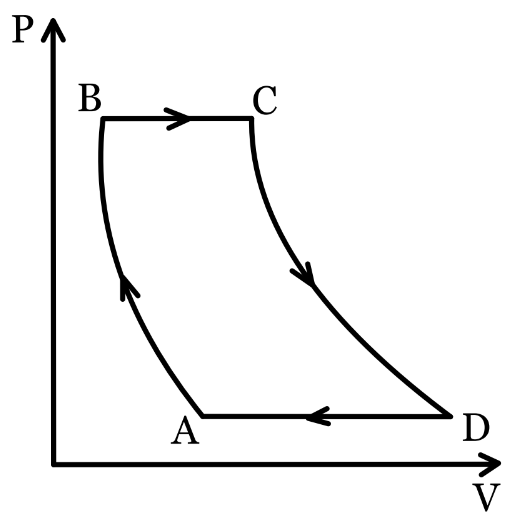
\includegraphics[width=0.6\textwidth]{BraytonCycle2.png}}
        \caption{Brayton Cycle}
        \label{fig:BraytonCycle}
    \end{subfigure}
    \hfill
    \begin{subfigure}[b]{0.5\textwidth}
    \centering
        \makebox[1.2\textwidth][l]{\hspace{-1.9cm} % Ajuste en caja para la segunda imagen
        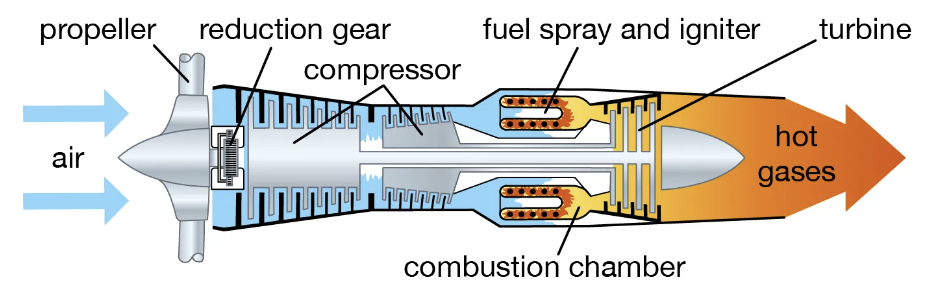
\includegraphics[width=1.25\textwidth]{turboprop.png}}
        \vspace{0.05cm} % Ajusta este valor para mover el caption hacia arriba o abajo
        \caption{Turboprop Architecture \cite{BritannicaInternalCombustion}}
        \label{fig:TurbopropArch}
    \end{subfigure}
\end{figure}



The global competitive demand for turboprop airplanes has led manufacturers like \textit{Avions de Transport Régional} (ATR) to prioritize efficiency and sustainability, as seen in the development of the "EVO" model. This aircraft, a hybrid that combines a highly efficient thermal engine with an electric motor powered by batteries, is designed to operate entirely on sustainable aviation fuel, with the goal of minimizing CO2 emissions, reducing maintenance costs, and improving overall performance \cite{ATREVOConcept}. The importance of thorough simulations in the aeronautical industry is underscored by incidents such as Boeing's "MCAS" system failure, which, due to ignored simulation warnings, caused two fatal crashes, claiming over 346 lives \cite{FrontlinePBSBoeing}. In Colombia, where large-scale aircraft manufacturing is limited, the aeronautical sector is primarily focused on maintenance, supported by the \textit{Corporación Industrial Aeronáutica Colombiana} (CIAC), which services imported aircraft for the Colombian Air Force (FAC) \cite{SemanaCIAC}. In addition, there is a growing emphasis on sustainable aviation fuels, as they could play a key role in reducing emissions and position Colombia as a potential exporter of palm oil-derived aviation fuel \cite{BonillaBiocombustibles} \cite{SanchezAceitePalma}.

Given these challenges, developing a computational tool capable of simulating the use of both conventional and alternative fuels (FNCER/SAF) in a turboprop engine is essential. This tool could analyze the torque transmitted to the propeller and optimize the engine's performance across varying airflow conditions. By modeling critical parameters—such as fuel mass, propeller thrust, and key aerothermodynamic factors—the tool aims to offer insights into fuel efficiency and engine behavior under different flight conditions, contributing to cost-effective and safe pre-operational testing. Such advancements could support the local aeronautical industry in developing competitive aircraft prototypes, facilitating manufacturing and maintenance processes, and aligning with environmental goals, ultimately benefiting organizations like ATR, CIAC, and the FAC \cite{QuinteroPoliticaAerea}.

%The manufacture of Turboprop airplanes is competitive and demanded worldwide. \textit{Avions de Transport Régional} (ATR) a leader in the manufacturing of this type of aircraft, is developing the "EVO" model, which seeks to merge a highly efficient thermal engine with an electric motor powered by a battery to optimize the size of the engine core and improve the overall efficiency of the propulsion system \cite{ATREVOConcept}. This twin-engine turboprop airplane, capable of using 100$\%$ Sustainable Aviation Fuel, aims to significantly reduce CO₂ emissions and direct maintenance costs while simultaneously improving aircraft performance.

%The importance of simulations in the aeronautical industry is evidenced in cases like Boeing's "MCAS" system. According to \cite{FrontlinePBSBoeing}, this automatic control system, designed to prevent aerodynamic stalls by pushing the nose of the airplane down, caused two 737 Max airplanes to crash unexpectedly, leaving over 346 deaths with no survivors. The FAA initiated an investigation that revealed that the MCAS had already been tested in different simulators with catastrophic results, but Boeing's negligence in ignoring these simulations led to the failed implementation of the software. 

%Figure \ref{fig:BoeingStock} shows how Boeing's stock has fallen in last year (2024) due to these investigations, demonstrating the importance of simulations to test new operating conditions safely and without risking lives.

%\begin{figure}[H]
%\centering
%\fbox{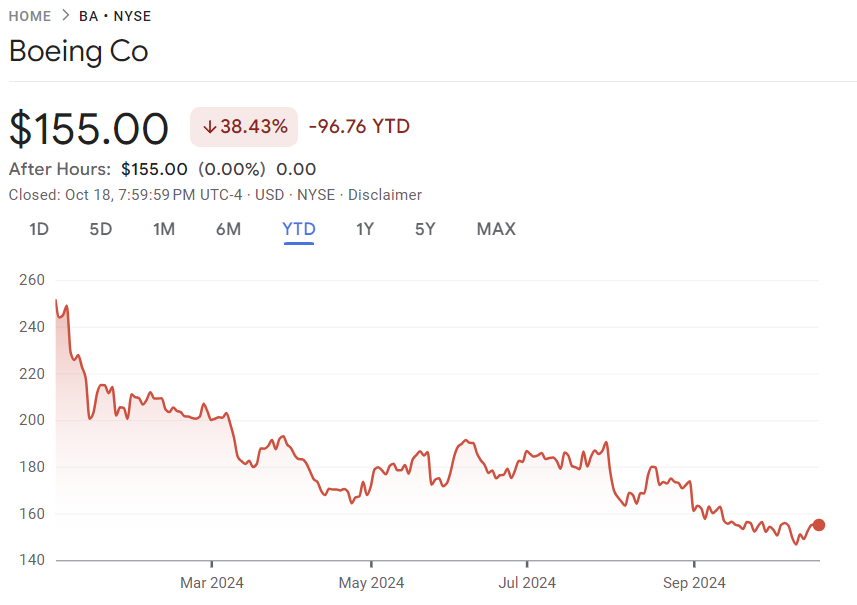
\includegraphics[width=0.5\textwidth]{BoeingStock.png}}
%\caption{Boeing Stock \cite{GoogleFinanceBoeing2024}}
%\label{fig:BoeingStock}
%\end{figure}

%In Colombia, turboprop airplanes and other types are sourced internationally, as large-scale manufacturing capabilities are absent domestically. The Colombian Air Force (FAC) fleet includes only one local model, the T-90, while larger aircraft, such as the Airbus C-295 and Lockheed Martin C-130, are imported and serviced in Colombian facilities. Maintenance is a key activity in the country's aeronautical industry, with companies like ATR, Airbus, and Lockheed Martin receiving this service from the \textit{Coorporación Industrial Aeronáutica Colombiana} (CIAC) \cite{SemanaCIAC}.

%Regarding fuel, there is an emerging focus on sustainable aviation fuels. According to Maristella Rodríguez, the commercial manager of KLM and Air France Colombia, by the year 2050, the aviation sector could contribute around 23\% of global carbon dioxide emissions if measures are not taken to reduce them \cite{BonillaBiocombustibles}. The implementation of biofuels can reduce environmental impact, and Colombia has the advantage of potentially exporting aviation fuel derived from palm oil, as announced by the executive president of Fedepalma, Nicolás Pérez Marulanda \cite{SanchezAceitePalma}.

%For these reasons, the development and coding of a computational tool capable of alternating between conventional and alternative fuels (FNCER / SAF) in the combustion chamber is essential. This tool would cover the total torque transmitted through the connecting shaft to the propeller and model its operation by adjusting its geometry across different airflow regimes. In this way, information can be obtained about the performance, behavior, and efficiency of the turboprop engine. A software capable of executing the above will guide the aeronautical industry towards the realistic implementation of pre-operational computational simulations.

%It will be crucial to vary different parameters, as sought in the ATR-EVO project, to establish the feasibility of implementing new technologies within an aircraft based on aerothermodynamic theoretical foundations, without risking lives or incurring additional expenses in prototype manufacturing.

%According to \cite{QuinteroPoliticaAerea}, thanks to their long-standing and developed aerospace industries, countries like the United States and those in the European Union save significantly on infrastructure and research costs. In this regard, the project could encourage the manufacture and maintenance of Colombian airplanes based on simulations that lead to a final product competitive in the market.

%The model seeks to balance how much fuel mass enters the engine and how much thrust the propeller produces, which makes the design project valuable. By studying the work produced by the engine and, in parallel, the aerodynamic behavior of the propeller, it is possible to know how much energy the system requires to function. This allows calculating the efficiency of the system and, by modeling the stages of the Turboprop architecture, it makes available to obtain a function with all those useful parameters (temperatures, pressures, work, forces, speeds, etc.), which together with the possibility of alternating fuels, implementing operational corrections, and evaluating different flight conditions, can play a fundamental role in companies like ATR, the CIAC, or the FAC itself within their manufacturing methodology, data analysis, and maintenance.


\section{Background}\label{sec:back}
With the advent of digital computers, the modeling of operational aviation systems based on data recording has become increasingly complex. This is due to the development of software capable of implementing and interpolating measured experimental data through Machine Learning. Most companies that manufacture airplanes, such as Rolls Royce, have carried out this type of characterization. They have specialized facilities for engine testing and data recording. These methods require exhaustive testing on experimental engine benches, which implies a significant expenditure of money, as it involves pushing engines to the limit conditions of the originally designed operation, as done in \cite{TakeOffBriefingRollsRoyce} to evaluate system performance.

However, implementing Machine Learning in this project was not feasible due to the lack of a complete and comprehensive database necessary for accurate model training. Given these limitations, it was more efficient in terms of time and resources to develop a computational model that could physically simulate engine. Unlike data-driven models, our approach relies on fundamental physical principles and information from existing literature, enabling practical testing and validation.

The development of software capable of simulating an airplane engine under specific flight conditions has been a subject of study mainly in research institutes or private companies, such as EngineSim with NASA \cite{BensonEngineSim}, GasTurb \cite{GasTurbSoftware}, or by the director of this work, who conducts a thermodynamic study of a PT6 engine with different biofuels \cite{Castellanos2019,Bayona2019PT6A}.

The GasTurb and EngineSim software programs are valuable tools for engineers in the gas turbine industry, engine manufacturing and maintenance, and aircraft structure development. Firstly, GasTurb simulates a wide array of gas turbine architectures for power generation, propulsion, and various airplane engine types, providing predefined models to kickstart custom designs and enabling thorough performance evaluations through model-based and empirical data \cite{GasTurbSoftware}. Similarly, NASA’s EngineSim software \cite{BensonEngineSim} facilitates propulsion analysis by adjusting mechanical and thermodynamic parameters, as well as flight speed and altitude, covering engine types such as Turbojet, Turbofan, Ramjet, and Jet with afterburner, with options for \textit{Design Mode} and \textit{Tunnel Test Mode} to modify variables or limit changes to flight conditions alone. Both programs offer users a comprehensive view of engine performance and efficiency, displaying the engine model being designed or tested, along with numerical values and graphical outputs for parameters like thrust, fuel flow, air flow, and engine weight. However, these programs share two significant limitations: neither accounts for the aerodynamic behavior of the propulsors, and as a result, neither includes turboprop engines among their available architectures. This limitation restricts their applicability for simulating the full range of operational dynamics in aviation engines, particularly for turboprops, where propeller aerodynamics play a critical role.

The work detailed in \cite{Castellanos2019,Bayona2019PT6A} involves a thermodynamic investigation into how the PT6A gas turbine engine, responds transiently across a range of operating conditions.It means that the effects of the propeller and aerodynamic factors were not applied in this model. The model used consists of differential and algebraic equations derived from mass balances, angular momentum, linear momentum, and energy in the engine components. That model was coded in Matlab-Simulink software, where the engine was additionally simulated with combinations of biodiesel and Jet-A1. To validate the simulation performed, the GasTurb software was used to obtain experimental values. The results obtained were positive since, when compared with GasTurb measurements, they were found to be at least as precise and reliable as those of that reference, specifically with a relative error below 10\% in most stages. Moreover, it was demonstrated that the model correctly predicted the maximum burner temperatures during the startup process and the pressure distribution across the engine stages; this suggests that the proposed approach could be useful in engine operations where fuel blends are applied. Finally, it is suggested as future work to couple kinetic combustion models, engine control, and efficiency.

Regarding BEMT, the approach taken in \cite{Castellanos2023Propeller}, where a computational strategy was developed to predict the aerodynamic performance of the Turboprop McCauley 4-blade propeller using BEM theory and CFD, revealed the practicality of BEMT in complex flow phenomena, being contrasted and validated by CFD and experimental results. However, it presents a complication in the torque results, since the measurements found showed variations in accuracy by BEMT compared to CFD. Additionally, along the article, the propeller was not connected to the engine because it was a fluid dynamics analysis for studying the behavior of the blades as an individual entity and not how it affected the propulsion aviation system as a whole, which, at the level of studying a complete engine–propeller system like the one managed by the Turboprop, made a precise exploration regarding the efficiencies of the complete system impossible. Therefore, the complete investigation of the Turboprop as a dual system through the BEMT and the engine's aerothermodynamics is an area of research that can begin to be forged based on the study done in \cite{Castellanos2019,Bayona2019PT6A} and \cite{Castellanos2023Propeller}.

Alternatives to BEMT are emerging that consider additional conditions that make the model more accurate compared to the operational reality. The analysis of non-uniform flow models is one of these alternatives and is related to rotor flight dynamics to understand the velocity distribution along the blade. It is used to capture the velocity distribution, as mentioned before, consider dynamic-transient effects, improve prediction accuracy, and control systems; being progress over the original BEMT. As clarified by \cite{Chen1989NonuniformInflow}, there are two classes of models used in the aeronautical industry: static and dynamic. The former have benefits due to their simplicity, facilitating their computational implementation but having the obstacle of only being able to model stationary or very similar situations; while the dynamic can be more computationally complex, allowing for the visualization of non-transient rotor behaviors such as speed changes or maneuvers, generating more realistic simulations that help control systems. For example, \cite{traub2016} introduced correction factors to BEMT that allow for modeling non-stationary rotor behaviors, such as speed variations and maneuvering effects, by accounting for changes in flow velocity and angle of attack along the blade. These adjustments improve the accuracy of BEMT in simulating realistic, dynamic conditions, supporting more effective control system designs.

The current absence of computational predictive models of a turboprop performance that unite both zones, thermal engine and propeller, in the state of the art is highlighted. On the contrary, the use of statistical regressions from flight-measured data is on the rise to obtain approximate functions through Machine Learning and thus model engine performance. For this reason, this computational model will be developed through Simulink, presenting a new paradigm for the industry thanks to the change in perspective from a statistical approach to a physical one, composed by operational variables; that is, a computational model that allows anticipating the mechanical operation of the engine in off design conditions.


\section{Objectives}
\textit{\bfseries To develop a computational simulation tool of the physicomathematical behavior of an aviation Turboprop engine subjected to different flight operating conditions and alternative fuels.}
\begin{enumerate}[itemsep=0.1pt]
    \item To formulate a physicomathematical model that integrates the BEMT for turbomachinery components and the thermodynamics of the Brayton cycle to represent the mechanical response of aviation Turboprop engines, including the correction factors of the BEMT.
    \item To code a modular computational tool in Matlab–Simulink that numerically solves the formulation resulting from objective 1.
    \item To evaluate the accuracy of the quantitative predictions obtained with respect to experimental data or other computational techniques used in the industry, available in specialized literature.
    \item To simulate the aerothermodynamic operation of the Turboprop engine in idle, taxiing, takeoff, and cruise regimes, operating with different conventional and alternative fuels.
\end{enumerate}

\section{Methodology Development}
The methodology is structured into eight phases as shown in  \autoref{fig:Methodology}, beginning with the mathematical formulation of the engine's thermodynamic components, including compressors, the combustion chamber, turbines, and shafts. Following this, XFOIL software is implemented to calculate parameters based on Traub's theory. The mathematical formulations are then coded into a Simulink model, integrating both the thermodynamic engine component and the propeller. Simulations and validations of the McCauley propeller and the engine's thermodynamic components are conducted, benchmarked against state-of-the-art data. Subsequently, the dynamic system, combining the engine and propeller, is integrated to simulate the complete turboprop engine, followed by its simulation and validation. Finally, simulations are performed with various fuel combinations to evaluate their effects on engine performance, ensuring a comprehensive and systematic approach throughout the process.

\begin{figure}[H]
\centering
\fbox{{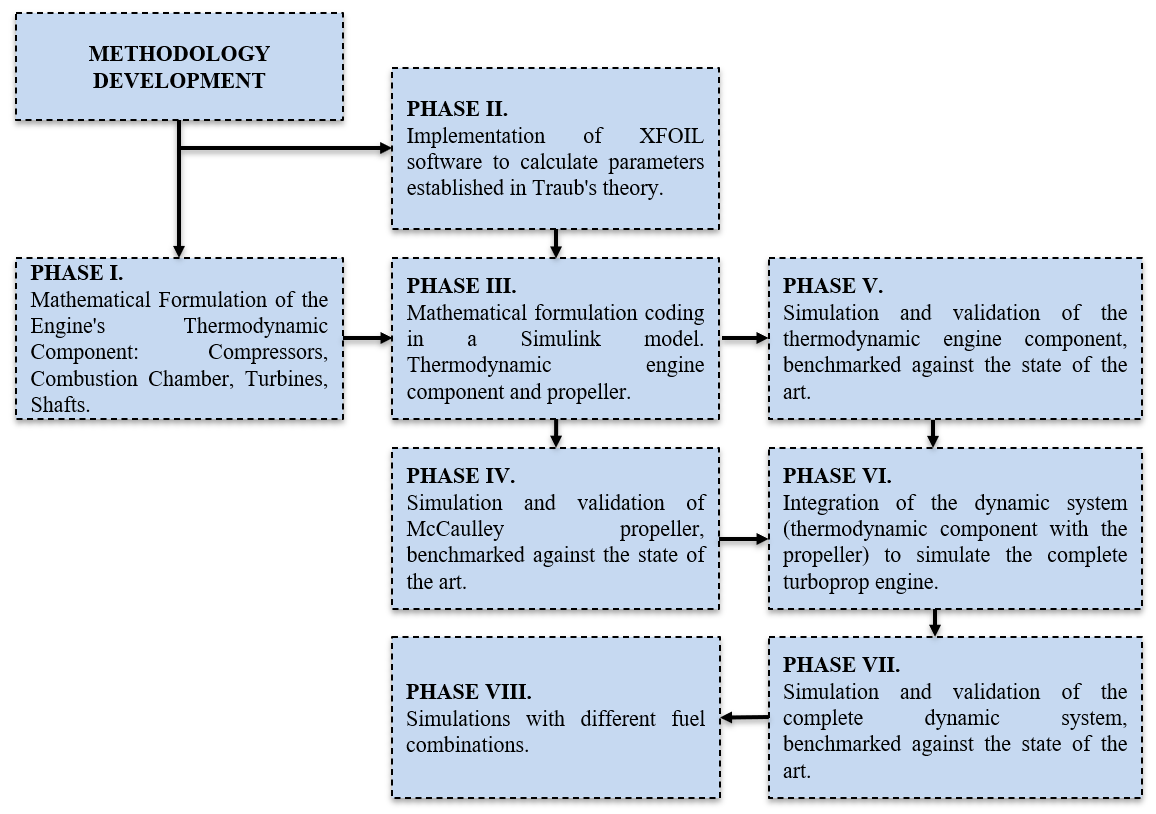
\includegraphics[width=0.65\textwidth]{METHODOLOGY.png}}}
\caption{Methodology Implementation}
\label{fig:Methodology}
\end{figure}

\section{Formulation Section: \emph{To formulate a physicomathematical model that integrates the BEMT for turbomachinery components and the
thermodynamics of the Brayton cycle to represent the mechanical response of PT6A with McCauley Propeler, including
the correction factors of the BEMT}}\label{sec:Method}

In this chapter, the development of the physicomathematical model that integrates BEMT with the thermodynamic principles of the Brayton cycle is described in order to represent the aerothermodynamic response of turboprop aviation engines through comprehensive mass, momentum, and energy balances. This methodology is applied to the PT6A engine and the McCauley propeller, coupling both systems at the power generation and propeller shafts to create a holistic model that accurately reflects operational conditions. By coupling the power generated in the engine to the propeller shaft, the model achieves realistic behavior under varying conditions, eliminating the need of some initial assumptions and aligning more closely with real-world performance.

Each component of the engine and propeller assembly—including compressors, the combustion chamber, turbines, the rotating shaft, and the propeller blades—is represented through a modular block structure. These blocks encompass the core principles required for analysis, including mass continuity, momentum exchange, and energy transformations across each stage, while also accounting for the aerodynamic forces and velocity distribution along the propeller blades. This framework enables the input of key operational parameters (e.g., rotational speed, upstream conditions) and calculates outputs relevant to the engine’s performance and efficiency. This structure provides adaptability by isolating component-specific calculations while ensuring they remain compatible within the broader system model.

By allowing each component to be analyzed independently within this modular framework, a realistic simulation of the turboprop engine’s aerothermodynamic behavior under varying flow regimes and operational conditions is achieved. The following sections detail the procedures used to fulfill the project’s objectives, including the complete modeling of the Brayton cycle, the engine’s thermal components, and the dynamic propeller mechanics.

It is important to clarify that the formulation was exclusively focused on modeling the propeller and the engine. Therefore, other variables or components that collectively make up a turboprop-powered aircraft were not considered. Additionally, the scope of the objectives was limited to this focus, meaning that any further modeling, such as the characterization of the wings, the aircraft's weight, or other factors, was beyond the purpose of this paper.


\subsection{PT6A Engine}

The PT6A engine consists of the following stages: axial compressors, a centrifugal compressor, a combustion chamber, turbines, the gas generation shaft, and the power generation shaft. 

As indicated in \cite{Castellanos2019,Bayona2019PT6A}, one of the main characteristics of this gas turbine engine is that it is mounted in reverse within the nacelle in most aeronautical installations. This allows the airflow to be directed toward the engine components in the same direction in which the aircraft is moving. Thus, the air passes over the exterior of the aircraft and the engine itself before entering the intake.

The design of the PT6A, as mentioned in \cite{Castellanos2019,Bayona2019PT6A}, is optimized to guide intake air into the engine through ducts that prevent exhaust gases from interfering with the airflow. Since the typical requirement is to provide clean and laminar air to the compressor to ensure maximum efficiency, the intake duct smoothly transitions from a direction opposite to the airflow to an axial direction aligned with the aircraft’s speed. Although the model developed in \cite{Castellanos2019,Bayona2019PT6A} is limited to ground operations, this project will consider various in-flight operations, including the air rarefaction processes that occur as air enters the engine.

\begin{figure}[H]
\centering
{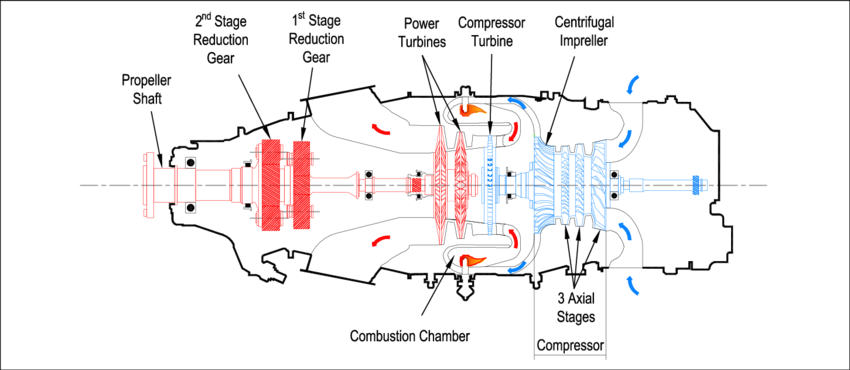
\includegraphics[width=0.75\textwidth]{turboprop_design.png}}
\caption{Pratt-Whitney PT6A-65 engine \cite{Bayona2019PT6A}}
\label{fig:PT6A-65}
\end{figure}

As illustrated in \autoref{fig:PT6A-65}, the engine has an intake that directs air to the compression stage, which consists of three axial compression stages and a single stage centrifugal compression. In these stages, the kinetic energy of the air is increased, raising its temperature and pressure. 

The axial compressor is composed of rotors, which add energy to the fluid, and stators, which redirect the airflow to maximize compression efficiency. As indicated in \cite{Castellanos2019,Bayona2019PT6A}, these rotating components reach speeds close to 40,000 revolutions per minute (RPM), increasing the air pressure between four \cite{PT6_VIDEO} and eight times \cite{Bayona2019PT6A} the inlet pressure according to the literature and flight data.

To understand the behavior of each axial compressor and other components, it is necessary to define the velocity triangle that governs the interactions between the rotors and stators at each stage of the compressor, as shown in \autoref{fig:tri_vel}. The velocity triangle will allow the calculation of the axial velocity, or the average velocity of the air, which is crucial for estimating the volumetric airflow passing through, with the air inlet angle as a known variable, as explained in \cite{Castellanos2019}.

\begin{figure}[H]
\centering
\fbox{{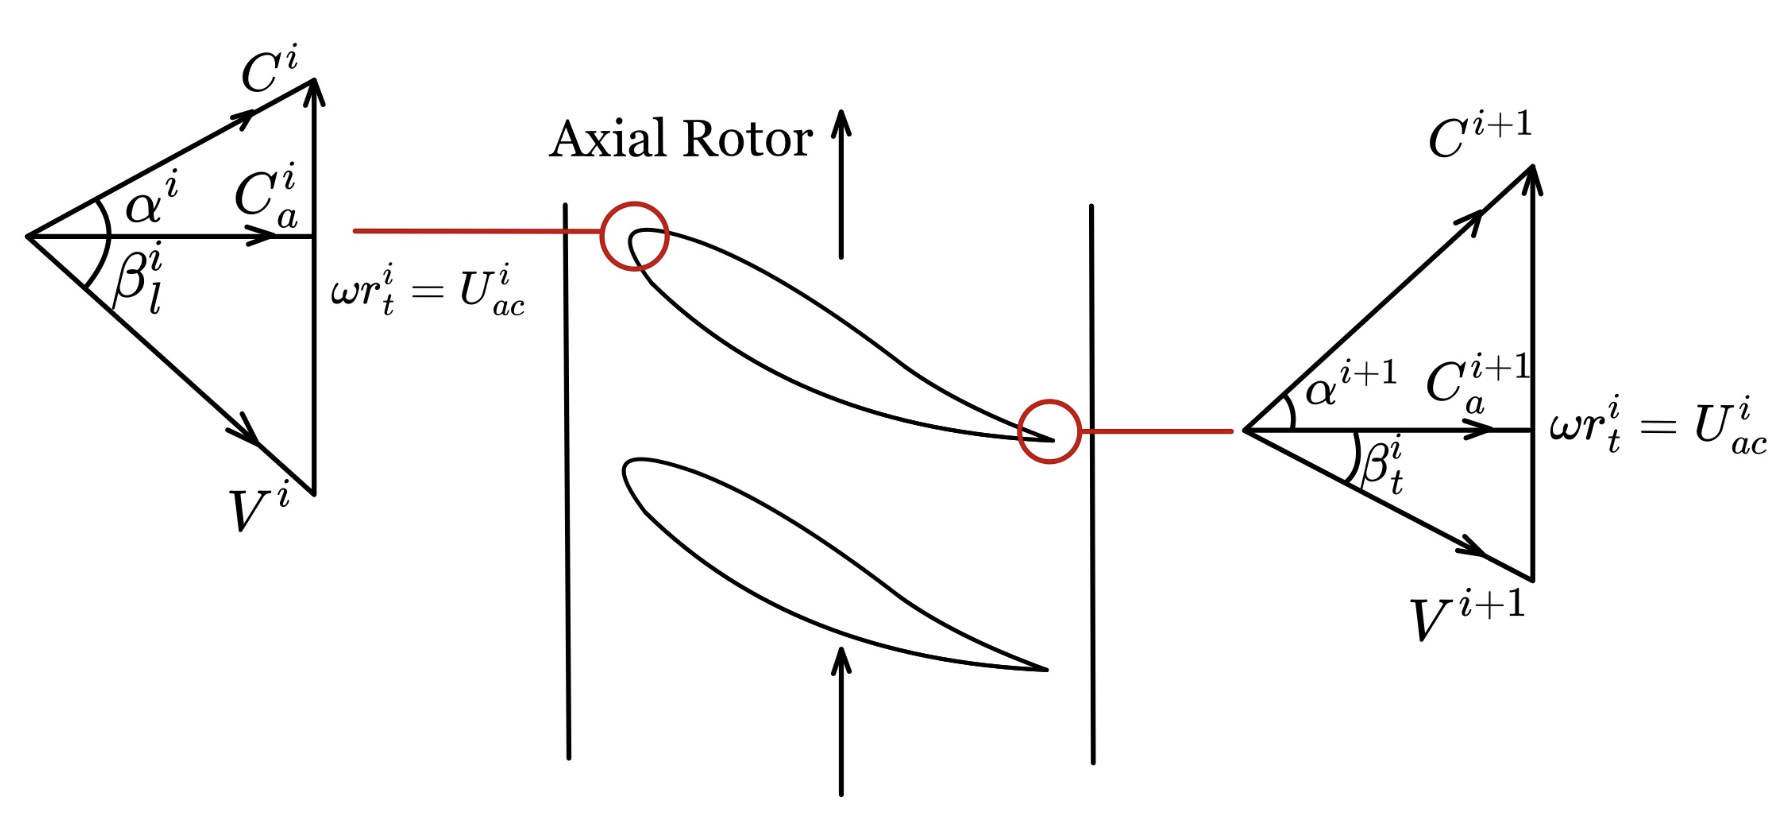
\includegraphics[width=0.8\textwidth]{TRI_VEL.png}}}
\caption{Euler Velocity Triangles for the Rotor}
\label{fig:tri_vel}
\end{figure}

For the first axial compressor, an angle $\alpha$ is assumed, which corresponds to the air inlet. However, for the other axial compression stages, this angle is set to 0°, as it is assumed that the stators are designed in such a way that the axial air velocity only has one component. This conditions are applied in ground conditions and low speeds.

After this compression, the air reaches the centrifugal compressor, which accelerates the air outward. In the centrifugal compressor, the same mass airflow is maintained due to the principle of mass conservation. Also, for the temperature and pressure at the outlet of the centrifugal compressor, it can be assumed that they are equal to the conditions at the outlet of the last axial compressor stage, given the system’s continuity. However, as mentioned in \cite{Castellanos2019,Bayona2019PT6A}, due to losses between centrifugal stages, this section is limited to a single stage before discharging the airflow. The airflow then exits the centrifugal section through the diffuser, a part of the engine that prepares the air for the combustion chamber. In this model, the representation of the diffuser has been omitted to simplify the engine’s compression section.

In the combustion chamber, injectors mix the fuel with compressed air, enabling the combustion that generates hot gases. At this section, high temperatures and pressures are produced because of the reaction between the fuel and the air. The mass flow rate within the combustion chamber is defined as the sum of the fuel flow and the compressor airflow, minus the flow that exits to the turbines.

As these gases expand and exit the combustion chamber, they pass through a series of turbines. The first turbine, connected to the gas generation shaft, uses the energy from the gases to drive the compressors, rotating at 40,000 RPM and ensuring the continuous compression of incoming air needed for sustained combustion. In the next two turbine stages, the thermal energy of the fluid is harnessed to drive the power generation shaft, which rotates at approximately 30,000 RPM. This shaft is responsible for generating the mechanical work needed to drive the propeller. The temperatures and pressures at the turbine inlet match the conditions at the combustion chamber outlet, ensuring efficient energy transfer between these stages.

After this process, the air is expelled into the atmosphere through the exhaust, allowing the air’s temperature and pressure to return to ambient conditions.


\subsubsection{Inlet and Axial Compression}

\autoref{fig:Inlet} and \autoref{fig:Axcomp} below present the balance and parameter model performed for the inlet and axial compression stages, along with their respective input and output variables.

%\centering
    \begin{figure}[H]
        \hspace{0.5cm}
        \begin{tikzpicture}
            % Definir estilos
            \tikzstyle{block} = [draw, fill=Goldenrod!30, rectangle, minimum height=6em, minimum width=10em, text centered, text width=3cm, rounded corners,]
            \tikzstyle{model} = [draw, fill=white!20, rectangle, minimum height=2em, minimum width=16em, text centered]
            \tikzstyle{input} = [node distance=-1.5cm, text centered]
            \tikzstyle{output} = [node distance=2cm, text centered]
            \tikzstyle{cloud} = [draw, ellipse,fill=white!20, node distance=3cm, minimum height=2em]
            \tikzstyle{line} = [draw, -latex']
    
            %\draw[dashed] (-10,0) rectangle (-1,8);
            
            \draw [dashed] (0,0) node[minimum height=5.05cm,minimum width=10.1cm,draw];
                   
            % Fondo amarillo
            %\filldraw [fill=yellow!20, draw=none] (0,0) rectangle (10,5);
            \draw (0,0) node[fill=black!20, minimum height=5cm,minimum width=10cm,draw=none];
            
            % Etiqueta del modelo 
            \node at (2.6,2.2) {Axial Compressor - Stage 1};
            %at (-10.6,0)
            
            % Bloque de cálculos
            \node [block] (calc) at (-3,-0.3){Calculations: $\rho, \text{$U_{ac}, C_{a}$} $\\ Parameters:\\ $\gamma$, \text{$R$}, \text{$C_{p}$} \\Geometry:\\ $\beta_{l}$, $\beta_{t}$, $r_{s}$, $r_{t}$, $\alpha$}
    
    
            % Entrada de velocidad
            \node (vel)at (-6.4,0.5){$\omega$};
            \node [below of=vel, node distance=-0.3cm](vel_text) {Angular Velocity };
            % Flecha ajustada para entrar en una parte específica del borde izquierdo
            \draw [->, -latex] (vel.east) -- ([yshift=0.8cm] calc.west);
    
            % Entrada de presión
            \node [input, below of=vel, node distance=0.8cm] (pressure) {$p_{(h)}$};
            \node [below of=pressure, node distance=-0.4cm] (pressure_text) {Pressure};
            \draw [->, -latex] (pressure.east) -- (calc.west);
    
            % Entrada de temperatura
            \node [input, below of=pressure, node distance=0.9cm] (temp) {$T_{(h)}$};
            \node [below of=temp, node distance=-0.4cm] (temp_text) {Temperature};
            \draw [->, -latex] (temp.east) -- ([yshift=-0.9cm] calc.west);
    
            % Caja de salida de velocidad axial
            %\node [model] (axial_out)  at (2.1,1.5) {$C_{a} = \frac{U_{ac}}{tan(\alpha)+tan(\beta_{l})}$};
            %\draw [->, -latex] (calc.east) -- (axial_out.west);
    
            % Caja de salida de flujo másico
            \node [model] (massflux_out) at (2.1,1.1) {$\dot{m}_{a} = C_{a}\pi(r_{t}^2-r_{s}^2)\rho$};
            \draw [->, -latex] (calc.east) -- (massflux_out.west);
    
            % Caja de salida de potencia
            \node [model,  below of=massflux_out, node distance=1cm] (potencia_out) {$\dot{W}_{1} = \dot{m}_{a}C_{a}U_{ac}tan(\beta_{l}-\beta_{t})$};
            \draw [->, -latex] (calc.east) -- (potencia_out.west);
    
              % Caja de salida de temperatura
            \node [model, below of=potencia_out, node distance=1cm] (temp_out) {$T_1= T_{(h)}+\frac{\dot{W}}{\dot{m}_{a}C_{p}}$};
            \draw [->, -latex] (calc.east) -- (temp_out.west);
    
            % Caja de salida de presión
            \node [model,  below of=temp_out, node distance=1cm] (pressure_out) {$p_1 = p_{(h)} \left[\frac{T_1}{T_{(h)}}  \right]^{\frac{\gamma}{\gamma-1}}$};
            \draw [->, -latex] (calc.east) -- (pressure_out.west);
    
            % Etiquetas de salida
            \node (massflux)at (6.4,1.1){$\dot{m}_{a}$};
            \node [below of=massflux, node distance=-0.4cm](massflux_text) {Air Mass Flux };
            \draw [->, -latex] (massflux_out.east) -- (massflux.west);
    
            \node [input, below of=massflux, node distance=1cm](potencia){$\dot{W}_{1}$};
            \node [below of=potencia, node distance=-0.4cm](potencia_text) {Power};
            \draw [->, -latex] (potencia_out.east) -- (potencia.west);
    
            \node [input, below of=potencia, node distance=1cm](temp){${T}_{1}$};
            \node [below of=temp, node distance=-0.4cm](temp_text) {Temperature};
            \draw [->, -latex] (temp_out.east) -- (temp.west);
            
            \node [input, below of=temp, node distance=1cm](pressure){${p}_{1}$};
            \node [below of=pressure, node distance=-0.4cm](pressure_text) {Pressure};
            \draw [->, -latex] (pressure_out.east) -- (pressure.west);  
        \end{tikzpicture}
    \caption{Inlet/First axial compressor stage}
    \label{fig:Inlet}
\end{figure}

\begin{figure}[H]
    \hspace{-0.25cm}
    \begin{tikzpicture}
            % Definir estilos
            \tikzstyle{block} = [draw, fill=Goldenrod!30, rectangle, minimum height=8em, minimum width=10em, text centered, text width=2.2cm, rounded corners,]
            \tikzstyle{model} = [draw, fill=white!20, rectangle, minimum height=2em, minimum width=16em, text centered]
            \tikzstyle{input} = [node distance=-1.5cm, text centered]
            \tikzstyle{output} = [node distance=2cm, text centered]
            \tikzstyle{cloud} = [draw, ellipse,fill=white!20, node distance=3cm, minimum height=2em]
            \tikzstyle{line} = [draw, -latex']
    
            %\draw[dashed] (-10,0) rectangle (-1,8);
            
            \draw [dashed] (0,0) node[minimum height=5.05cm,minimum width=11.1cm,draw];
                   
            % Fondo amarillo
            %\filldraw [fill=black!20, draw=none] (0,0) rectangle (10,5);
            \draw (0,0) node[fill=black!20, minimum height=5cm,minimum width=11cm,draw=none];
            
            % Etiqueta del modelo 
            \node at (2.8,2.2) {Axial Compressor - Stage 2-3};
            %at (-10.6,0)
            
            % Bloque de cálculos
            \node [block] (calc) at (-3.5,-0.3){Calculations: $\rho^{i}, \text{$U_{ac}^{i}, C_{a}^{i}$} $ Parameters: $\gamma$, \text{$R$}, \text{$C_{p}$} Geometry: $\beta_{l}^{i}$, $\beta_{t}^{i}$}
    
            % Entrada de flujo masico
            \node (flux)at (-7.4,0.9){$\dot{m}_{a}$};
            \node [below of=flux, node distance=-0.4cm](flux_text) {Air Mass Flux };
            \draw [->, -latex] (flux.east) -- ([yshift=1.2cm] calc.west);
    
            % Entrada de velocidad
            \node [input, below of=flux, node distance=0.8cm] (vel){$\omega$};
            \node [below of=vel, node distance=-0.4cm](vel_text) {Angular Velocity };
            \draw [->, -latex] (vel.east) -- ([yshift=0.4cm] calc.west);
    
            % Entrada de presión
            \node [input, below of=vel, node distance=0.8cm] (pressure) {$p^{i-1}$};
            \node [below of=pressure, node distance=-0.4cm] (pressure_text) {Pressure};
            \draw [->, -latex] (pressure.east) -- ([yshift=-0.4cm]calc.west);
    
            % Entrada de temperatura
            \node [input, below of=pressure, node distance=0.9cm] (temp) {$T^{i-1}$};
            \node [below of=temp, node distance=-0.4cm] (temp_text) {Temperature};
            \draw [->, -latex] (temp.east) -- ([yshift=-1.3cm] calc.west);
    
            % Caja de salida de velocidad axial
            %\node [model] (axial_out)  at (2.1,1.5) {$C_{a} = \frac{U_{ac}}{tan(\alpha)+tan(\beta_{l})}$};
            %\draw [->, -latex] (calc.east) -- (axial_out.west);
    
            % Caja de salida de flujo másico
            \node [model] (massflux_out) at (2.4,1.1) {$\dot{m}_{a} = \dot{m}_{a}$};
            \draw [->, -latex] (calc.east) -- (massflux_out.west);
    
            % Caja de salida de potencia
            \node [model,  below of=massflux_out, node distance=1cm] (potencia_out) {$\dot{W}^{i} = \dot{m}_{a}U_{ac}^{i}tan(\beta_{l}^{i}-\beta_{t}^{i})C_{a}^{i}$};
            \draw [->, -latex] (calc.east) -- (potencia_out.west);
            %(\frac{\dot{m}}{\rho*\pi*(r_{l}^{i}^2-r_{t}^{i}^2)})^2
    
                
              % Caja de salida de temperatura
            \node [model, below of=potencia_out, node distance=1cm] (temp_out) {$T^{i} = T^{i-1}+\frac{\dot{W}^{i}}{\dot{m}C_{p}}$};
            \draw [->, -latex] (calc.east) -- (temp_out.west);
    
            % Caja de salida de presión
            \node [model,  below of=temp_out, node distance=1cm] (pressure_out) {$p^{i} = p^{i-1} \left[\frac{T^{i}}{T^{i-1}}  \right]^{\frac{\gamma}{\gamma-1}}$};
            \draw [->, -latex] (calc.east) -- (pressure_out.west);
    
            % Etiquetas de salida
            \node (massflux)at (6.8,1.1){$\dot{m}_{a}$};
            \node [below of=massflux, node distance=-0.4cm](massflux_text) {Air Mass Flux };
            \draw [->, -latex] (massflux_out.east) -- (massflux.west);
    
            \node [input, below of=massflux, node distance=1cm](potencia){$\dot{W}^{i}$};
            \node [below of=potencia, node distance=-0.4cm](potencia_text) {Power};
            \draw [->, -latex] (potencia_out.east) -- (potencia.west);
    
            \node [input, below of=potencia, node distance=1cm](temp){${T}^{i}$};
            \node [below of=temp, node distance=-0.4cm](temp_text) {Temperature};
            \draw [->, -latex] (temp_out.east) -- (temp.west);
            
            \node [input, below of=temp, node distance=1cm](pressure){${p}^{i}$};
            \node [below of=pressure, node distance=-0.4cm](pressure_text) {Pressure};
            \draw [->, -latex] (pressure_out.east) -- (pressure.west);      
        \end{tikzpicture}
    \caption{Last axial compression stages model}
    \label{fig:Axcomp}
\end{figure}

\autoref{tab:axial_compressors} presents the geometry of the axial compressors, detailing values for the inlet and stages 2 and 3. Parameters such as the tip radius ($r_{t,1}$) and root radius ($r_{s,1}$), as well as the angles $\beta_1$, $\beta_t$, and $\alpha$, are provided from previous works \cite{Castellanos2019,Bayona2019PT6A}. This information is essential for analyzing the aerodynamic behavior and efficiency across different stages of the compressor.

\begin{table}[h!]
    \centering
    \begin{tabular}{|l|c|c|c|c|}
        \hline
        \textbf{Blade} & \textbf{Symbol} & \textbf{1st-Inlet} & \textbf{2nd-stage} & \textbf{3rd-stage} \\
        \hline
        Tip radius [m] & $r_{t,1}$ & 0.10 & 0.096 & 0.092 \\
        Root radius [m] & $r_{s,1}$ & 0.072 & 0.076 & 0.08 \\
        Inlet angle [°] & $\beta_1$ & 61.5 & 57.85 & 57.1 \\
        Exit angle [°] & $\beta_t$ & 50.5 & 43.5 & 36.2 \\
        Air angle [°] & $\alpha$ & 61.5 & N/A & N/A \\
        \hline
    \end{tabular}
    \caption{Geometry of the Axial Compressors}
    \label{tab:axial_compressors}
\end{table}

\subsubsection{Centrifugal Compression}

\autoref{fig:Centcomp} below present the balance and parameter model performed for the single stage centrifugal compressor, along with their respective input and output variables. Some of the initial variables were obtained in the previous stages blocks, such as pressure, temperature and air mass flux.


\begin{figure}[H]
    \hspace{-1.5cm}
    \begin{tikzpicture}
            % Definir estilos
            \tikzstyle{block} = [draw, fill=Goldenrod!30, rectangle, minimum height=6em, minimum width=10em, text centered, text width=2.2cm, rounded corners,]
            \tikzstyle{model} = [draw, fill=white!20, rectangle, minimum height=2em, minimum width=26em, text centered]
            \tikzstyle{input} = [node distance=-1.5cm, text centered]
            \tikzstyle{output} = [node distance=2cm, text centered]
            \tikzstyle{cloud} = [draw, ellipse,fill=white!20, node distance=3cm, minimum height=2em]
            \tikzstyle{line} = [draw, -latex']
    
    
            
            %\draw[dashed] (-10,0) rectangle (-1,8);
            
            \draw [dashed] (1.3,-0.5) node[minimum height=6.07cm,minimum width=13.75cm,draw];
                   
            % Fondo amarillo
            %\filldraw [fill=yellow!20, draw=none] (0,0) rectangle (10,5);
            \draw (1.3,-0.5) node[fill=black!20, minimum height=6cm,minimum width=13.7cm,draw=none];
            
            % Etiqueta del modelo 
            \node at (5.5,2.2) {Centrifugal Compressor};
            %at (-10.6,0)
            
            % Bloque de cálculos
            \node [block] (calc) at (-3.5,-0.9){Calculations: $\rho^{i}, \text{$ C_{1}$}, \text{$ C_{2}$} $ Parameters: $\gamma$, \text{$R$}, \text{$C_{p}$} Geometry: $b_{1}$, $b_{2}$, $\beta_{l}^{i}$, $\beta_{t}^{i}$, $r_{s}^{i}$, $r_{t}^{i}$}
    
            % Entrada de flujo masico
            \node (flux)at (-7.4,0.3){$\dot{m}_{a}$};
            \node [below of=flux, node distance=-0.4cm](flux_text) {Air Mass Flux };
            \draw [->, -latex] (flux.east) -- ([yshift=1.2cm] calc.west);
    
            % Entrada de velocidad
            \node [input, below of=flux, node distance=0.8cm] (vel){$\omega$};
            \node [below of=vel, node distance=-0.4cm](vel_text) {Angular Velocity };
            \draw [->, -latex] (vel.east) -- ([yshift=0.4cm] calc.west);
    
            % Entrada de presión
            \node [input, below of=vel, node distance=0.8cm] (pressure) {$p^{i-1}$};
            \node [below of=pressure, node distance=-0.4cm] (pressure_text) {Pressure};
            \draw [->, -latex] (pressure.east) -- ([yshift=-0.4cm]calc.west);
    
            % Entrada de temperatura
            \node [input, below of=pressure, node distance=0.9cm] (temp) {$T^{i-1}$};
            \node [below of=temp, node distance=-0.4cm] (temp_text) {Temperature};
            \draw [->, -latex] (temp.east) -- ([yshift=-1.3cm] calc.west);
    
            % Caja de salida de velocidad axial
            %\node [model] (axial_out)  at (2.1,1.5) {$C_{a} = \frac{U_{ac}}{tan(\alpha)+tan(\beta_{l})}$};
            %\draw [->, -latex] (calc.east) -- (axial_out.west);
    
            % Caja de salida de flujo másico
            \node [model] (massflux_out) at (3.4,1.1) {$\dot{m}_{a} = \dot{m}_{a}$};
            \draw [->, -latex] (calc.east) -- (massflux_out.west);
    
            % Caja de salida de flujo volumetrico
            \node [model, below of=massflux_out, node distance=1cm] (volflux_out) {$\dot{V} = 2\pi C_{1}r_{s}^{i}b_{1} = 2\pi C_{2}r_{t}^{i}b_{2}$};
            \draw [->, -latex] (calc.east) -- (volflux_out.west);
    
            % Caja de salida de potencia
            \node [model,  below of=volflux_out, node distance=1cm] (potencia_out) {$\dot{W}^{i} = \rho^{i}\omega\dot{V}[r_{t}( \omega r_{t} -\frac{C_{2}}{tan(\beta_{l}^{i})})-r_{s}( \omega r_{s}-\frac{C_{1}}{tan(\beta_{t}^{i})})]$};
            \draw [->, -latex] (calc.east) -- (potencia_out.west);
            %(\frac{\dot{m}}{\rho*\pi*(r_{l}^{i}^2-r_{t}^{i}^2)})^2
    
                
              % Caja de salida de temperatura
            \node [model, below of=potencia_out, node distance=1cm] (temp_out) {$T^{i} = T^{i-1}+\frac{\dot{W}^{i}}{\dot{m}_{a}C_{p}}$};
            \draw [->, -latex] (calc.east) -- (temp_out.west);
    
            % Caja de salida de presión
            \node [model,  below of=temp_out, node distance=1cm] (pressure_out) {$p^{i} = p^{i-1} \left[\frac{T^{i}}{T^{i-1}}  \right]^{\frac{\gamma}{\gamma-1}}$};
            \draw [->, -latex] (calc.east) -- (pressure_out.west);
    
            % Etiquetas de salida
            \node (massflux)at (9.5,1.1){$\dot{m}_{a}$};
            \node [below of=massflux, node distance=-0.4cm](massflux_text) {Air Mass Flux };
            \draw [->, -latex] (massflux_out.east) -- (massflux.west);
    
            \node [input, below of=massflux, node distance=1cm](volflux){$\dot{V}$};
            \node [below of=volflux, node distance=-0.4cm](volflux_text) {Volumetric Flux};
            \draw [->, -latex] (volflux_out.east) -- (volflux.west);
            
            \node [input, below of=volflux, node distance=1cm](potencia){$\dot{W}^{i}$};
            \node [below of=potencia, node distance=-0.4cm](potencia_text) {Power};
            \draw [->, -latex] (potencia_out.east) -- (potencia.west);
    
            \node [input, below of=potencia, node distance=1cm](temp){${T}^{i}$};
            \node [below of=temp, node distance=-0.4cm](temp_text) {Temperature};
            \draw [->, -latex] (temp_out.east) -- (temp.west);
            
            \node [input, below of=temp, node distance=1cm](pressure){${p}^{i}$};
            \node [below of=pressure, node distance=-0.4cm](pressure_text) {Pressure};
            \draw [->, -latex] (pressure_out.east) -- (pressure.west);
        \end{tikzpicture}
    \caption{Centrifugal Compression Model}
    \label{fig:Centcomp}
    \end{figure}
The table below (\autoref{tab:centrifugal_compressors}) shows the geometry of the centrifugal compressors for Stage 1. It includes values for the tip radius ($r_{t,1}$), root radius ($r_{s,1}$), and blade heights ($b_1$ and $b_2$), along with the blade angles $\beta_1$ and $\beta_t$. These parameters are key to understanding the structural and aerodynamic characteristics of the centrifugal compressor stage.

\begin{table}[h!]
    \centering
    \begin{tabular}{|l|c|c|}
        \hline
        \textbf{Blade} & \textbf{Symbol} & \textbf{One-Stage} \\
        \hline
        Tip radius [m] & $r_{t,1}$ & 0.117 \\
        Root radius [m] & $r_{s,1}$ & 0.092 \\
        First blade height [m] & $b_1$ & 0.0201 \\
        Second blade height [m] & $b_2$ & 0.02 \\
        Inlet angle [°] & $\beta_1$ & 38 \\
        Exit angle [°] & $\beta_t$ & 40 \\
        \hline
    \end{tabular}
    \caption{Geometry of the Centrifugal Compressors}
    \label{tab:centrifugal_compressors}
\end{table}

\subsubsection{Combustion Chamber}
\autoref{fig:CombChamber} below present the balance and parameter model performed for the combustion chamber. Some of its parameters are air properties and also a single fuel property, $LHV$.
\begin{figure}[H]
\hspace{1.5cm}
    \begin{tikzpicture}
        % Definir estilos
        \tikzstyle{block} = [draw, fill=Goldenrod!30, rectangle, minimum height=9em, minimum width=7em, text centered, text width=2.2cm, rounded corners,]
        \tikzstyle{model} = [draw, fill=white!20, rectangle, minimum height=2em, minimum width=18em, text centered]
        \tikzstyle{input} = [node distance=-1.5cm, text centered]
        \tikzstyle{output} = [node distance=2cm, text centered]
        \tikzstyle{cloud} = [draw, ellipse,fill=white!20, node distance=3cm, minimum height=2em]
        \tikzstyle{line} = [draw, -latex']


        
        %\draw[dashed] (-10,0) rectangle (-1,8);
        
        \draw [dashed] (1.3,-0.5) node[minimum height=5.1cm,minimum width=10.1cm,draw];
               
        % Fondo amarillo
        %\filldraw [fill=yellow!20, draw=none] (0,0) rectangle (10,5);
        \draw (1.3,-0.5) node[fill=black!20, minimum height=5cm,minimum width=10cm,draw=none];       
        
        % Etiqueta del modelo 
        \node at (4.5,1.5) {Combustion Chamber};
        %at (-10.6,0)
        
        % Bloque de cálculos
        \node [block] (calc) at (-2,-0.9){Calculations: $\rho^{i} $ \\Parameters: \text{$R$}, \text{$C_{p}, LHV$} Geometry: \\$V_{c}$}

        % Entrada de flujo masico
        \node (flux)at (-5,0.3){$\dot{m}_{a}$};
        \node [below of=flux, node distance=-0.4cm](flux_text) {Air Mass Flux};
        \draw [->, -latex] (flux.east) -- ([yshift=1.2cm] calc.west);

        % Entrada de velocidad
        \node [input, below of=flux, node distance=0.8cm] (vel){$\dot{m}_{f}$};
        \node [below of=vel, node distance=-0.4cm](vel_text) {Fuel Mass Flux};
        \draw [->, -latex] (vel.east) -- ([yshift=0.4cm] calc.west);

        % Entrada de presión
        \node [input, below of=vel, node distance=0.8cm] (pressure) {$p^{i-1}$};
        \node [below of=pressure, node distance=-0.4cm] (pressure_text) {Pressure};
        \draw [->, -latex] (pressure.east) -- ([yshift=-0.4cm]calc.west);

        % Entrada de temperatura
        \node [input, below of=pressure, node distance=0.9cm] (temp) {$T^{i-1}$};
        \node [below of=temp, node distance=-0.4cm] (temp_text) {Temperature};
        \draw [->, -latex] (temp.east) -- ([yshift=-1.3cm] calc.west);

        % Caja de salida de velocidad axial
        %\node [model] (axial_out)  at (2.1,1.5) {$C_{a} = \frac{U_{ac}}{tan(\alpha)+tan(\beta_{l})}$};
        %\draw [->, -latex] (calc.east) -- (axial_out.west);

        % Caja de salida de flujo másico
        \node [model] (massflux_out) at (3,0.1) {$\dot{m}_{g} = \dot{m}_{a}+\dot{m}_{f}$};
        \draw [->, -latex] (calc.east) -- (massflux_out.west);

        % Caja de salida de temperatura
        \node [model, below of=massflux_out, node distance=1cm] (temp_out) {$\frac{dT^{i}}{dt} = \frac{\dot{m}_{f}LHV+C_{p}(T^{i-1}\dot{m}_{a}-T^{i}(\dot{m}_{f}+\dot{m}_{a}))}{C_{p}V_{c}\rho}$};
        \draw [->, -latex] (calc.east) -- (temp_out.west);

        % Caja de salida de presión
        \node [model,  below of=temp_out, node distance=1cm] (pressure_out) {$p^{i} = p^{i-1}$};
        \draw [->, -latex] (calc.east) -- (pressure_out.west);

        % Etiquetas de salida
        \node (massflux)at (7.8,0.1){$\dot{m}_{g}$};
        \node [below of=massflux, node distance=-0.4cm](massflux_text) {Gas Mass Flux };
        \draw [->, -latex] (massflux_out.east) -- (massflux.west);

        \node [input, below of=massflux, node distance=1cm](temp){${T}^{i}$};
        \node [below of=temp, node distance=-0.4cm](temp_text) {Temperature};
        \draw [->, -latex] (temp_out.east) -- (temp.west);

        \node [input, below of=temp, node distance=1cm](pressure){${p}^{i}$};
        \node [below of=pressure, node distance=-0.4cm](pressure_text) {Pressure};
        \draw [->, -latex] (pressure_out.east) -- (pressure.west); 
        \end{tikzpicture}
    \caption{Combustion Chamber Model}
    \label{fig:CombChamber}
\end{figure} 

The designed volume of the combustion chamber is 0.02883 m\(^3\), a dimension chosen to optimize the fuel-air mixing ratio and maintain appropriate pressure levels for efficient combustion within the PT6A engine.

\subsubsection{Turbine Section}
\autoref{fig:Turbine} below present the balance and parameter model performed for the turbine stages. This section ends the whole engine system.

\begin{figure}[H]
    \hspace{1.25cm}
    \begin{tikzpicture}
        % Definir estilos
        \tikzstyle{block} = [draw, fill=Goldenrod!30, rectangle, minimum height=8em, minimum width=10em, text centered, text width=2.5cm, rounded corners,]
        \tikzstyle{model} = [draw, fill=white!20, rectangle, minimum height=2em, minimum width=16em, text centered]
        \tikzstyle{input} = [node distance=-1.5cm, text centered]
        \tikzstyle{output} = [node distance=2cm, text centered]
        \tikzstyle{cloud} = [draw, ellipse,fill=white!20, node distance=3cm, minimum height=2em]
        \tikzstyle{line} = [draw, -latex']


        
        %\draw[dashed] (-10,0) rectangle (-1,8);
        
        \draw [dashed] (1.3,-0.5) node[minimum height=5.1cm,minimum width=10.1cm,draw];
               
        % Fondo amarillo
        %\filldraw [fill=black!20, draw=none] (0,0) rectangle (10,5);
        \draw (1.3,-0.5) node[fill=black!20, minimum height=5cm,minimum width=10cm,draw=none];
        
        
        % Etiqueta del modelo 
        \node at (4.2,1.5) {Turbine - Stage 1-2-3};
        %at (-10.6,0)
        
        % Bloque de cálculos
        \node [block] (calc) at (-1.8,-1){Calculations:\\ $\rho^{i}$ \\ Parameters: $\gamma$, \text{$R_{p}^{i}$}, \text{$R$}, \text{$C_{p}$} Geometry: \\$\beta_{l}^{i}$, $\beta_{t}^{i}$, $r_{s}^{i}$, $r_{t}^{i}$}

        % Entrada de velocidad
        \node (vel)at (-5.2,-0.3){$\omega$};
        \node [below of=vel, node distance=-0.4cm](vel_text) {Angular Velocity };
        \draw [->, -latex] (vel.east) -- ([yshift=0.7cm] calc.west);

        % Entrada de presión
        \node [input, below of=vel, node distance=0.8cm] (pressure) {$p^{i-1}$};
        \node [below of=pressure, node distance=-0.4cm] (pressure_text) {Pressure};
        \draw [->, -latex] (pressure.east) -- ([yshift=-0.1cm]calc.west);

        % Entrada de temperatura
        \node [input, below of=pressure, node distance=0.9cm] (temp) {$T^{i-1}$};
        \node [below of=temp, node distance=-0.4cm] (temp_text) {Temperature};
        \draw [->, -latex] (temp.east) -- ([yshift=-1cm] calc.west);

        % Caja de salida de velocidad axial
        %\node [model] (axial_out)  at (2.1,1.5) {$C_{a} = \frac{U_{ac}}{tan(\alpha)+tan(\beta_{l})}$};
        %\draw [->, -latex] (calc.east) -- (axial_out.west);

        % Caja de salida de temperatura
        \node [model] (temp_out) at (3.3,0.6) {$T^{i} = T^{i-1}\left[{R_{p}^{i}}  \right]^{\frac{\gamma}{\gamma-1}}$};
        \draw [->, -latex] (calc.east) -- (temp_out.west);

        % Caja de salida de presión
        \node [model,  below of=temp_out, node distance=1cm] (pressure_out) {$p^{i} = p^{i-1} R_{p}^{i} $};
        \draw [->, -latex] (calc.east) -- (pressure_out.west);

        % Caja de salida de flujo másico
        \node [model, below of=pressure_out, node distance=1cm] (massflux_out){$\dot{m}_{t} = \frac{\pi \rho^{i} \Delta T^{i} C_{p} ((r_{t}^{i})^{2}-(r_{s}^{i})^{2})}{\omega[tan(\beta_{l}^{i})-tan(\beta_{t}^{i})]r_{s}^{i}} $};
        \draw [->, -latex] (calc.east) -- (massflux_out.west);


        % Caja de salida de potencia
        \node [model,  below of=massflux_out, node distance=1cm] (potencia_out) {$\dot{W}^{i} = \dot{m}_{t} \Delta T^{i} C_{p}$};
        \draw [->, -latex] (calc.east) -- (potencia_out.west);
        %(\frac{\dot{m}}{\rho*\pi*(r_{l}^{i}^2-r_{t}^{i}^2)})^2

            
          

        % Etiquetas de salida
        \node (temp)at (8,0.6){${T}^{i}$};
        \node [below of=temp, node distance=-0.4cm](temp_text) {Temperature};
        \draw [->, -latex] (temp_out.east) -- (temp.west);

        \node [input, below of=temp, node distance=1cm](pressure){${p}^{i}$};
        \node [below of=pressure, node distance=-0.4cm](pressure_text) {Pressure};
        \draw [->, -latex] (pressure_out.east) -- (pressure.west);
        
        \node [input, below of=pressure, node distance=1cm](massflux){$\dot{m}_{t}$};
        \node [below of=massflux, node distance=-0.4cm](massflux_text) {Turbine Mass Flux };
        \draw [->, -latex] (massflux_out.east) -- (massflux.west);

        \node [input, below of=massflux, node distance=1cm](potencia){$\dot{W}^{i}$};
        \node [below of=potencia, node distance=-0.4cm](potencia_text) {Power};
        \draw [->, -latex] (potencia_out.east) -- (potencia.west);
    \end{tikzpicture}
    \caption{Turbine Model}
    \label{fig:Turbine}
\end{figure}

\autoref{tab:combined_turbine_geometry} presents the geometry of the turbines. \autoref{tab:gas_generation_turbine} shows the parameters for the gas generation turbine, and \autoref{tab:power_generation_turbine} presents the parameters for the power generation turbines in stages 1 and 2. These tables specify the tip radius ($r_{t,1}$) and root radius ($r_{s,1}$), as well as the blade angles $\beta_1$ and $\beta_t$. This data is crucial for assessing the aerodynamic performance and efficiency of the turbines under operational conditions.

\begin{table}[h!]
    \centering
    
    % Subtabla de la Turbina de Generación de Gas
    \begin{subtable}[t]{0.475\textwidth}
        \centering
        \begin{tabular}{|l|c|c|}
            \hline
            \textbf{Geometry} & \textbf{Symbol} & \textbf{One-Stage (1st-Stage)} \\
            \hline
            Tip radius [m] & $r_{t,1}$ & 0.117 \\
            Root radius [m] & $r_{s,1}$ & 0.092 \\
            Inlet angle [°] & $\beta_1$ & -20 \\
            Exit angle [°] & $\beta_t$ & 80 \\
            Compression Ratio & $(R_{\text{p}})_g$ & 1/3.03\\
            \hline
        \end{tabular}
        \caption{Geometry of the Gas Generation Turbine}
        \label{tab:gas_generation_turbine}
    \end{subtable}
    \hfill
    % Subtabla de las Turbinas de Generación de Potencia
    \begin{subtable}[t]{0.475\textwidth}
        \centering
        \begin{tabular}{|l|c|c|c|}
            \hline
            \textbf{Geometry} & \textbf{Symbol} & \textbf{2nd-Stage} & \textbf{3rd-Stage} \\
            \hline
            Tip radius [m] & $r_{t,1}$ & 0.125 & 0.142 \\
            Root radius [m] & $r_{s,1}$ & 0.09 & 0.088 \\
            Inlet angle [°] & $\beta_1$ & -20 & -20 \\
            Exit angle [°] & $\beta_t$ & 43 & 43 \\
            Compression Ratio & $(R_{\text{p}})_P$ & 1/1.47 & 1/1.47\\
            \hline
        \end{tabular}
        \caption{Geometry of the Power Generation Turbines}
        \label{tab:power_generation_turbine}
    \end{subtable}
        \captionsetup{justification=centering} % Centra el título general
    \vspace{10pt}
    \caption{Geometry of Turbines}
    \label{tab:combined_turbine_geometry}
\end{table}

\subsubsection{Rotating Shafts}
An angular momentum balance is applied to both shafts, gas generation and power generation shafts. To do this, the angular velocity of the shaft, its moment of inertia, and the applied torques are defined. The moment of inertia of the gas generation stage shaft is approximately 0.12 kg·m², and for the power generation stage shaft is 0.06 kg·m². In the turboprop PT6A architecture, the first turbine stage drives the engine's gas generator, while the remaining turbine stages are dedicated to powering the propeller and providing thrust for the aircraft. All the above, could be describe as:

\begin{equation}
I \frac{d\omega}{dt} = \sum M_{\text{input}} + M_{\text{load}} - M_{\text{friction}} - M_{\text{other resistances}}
\end{equation}

\subsection{McCauley Propeller}

The McCauley propeller \cite{mccauley2023techguide} is an essential mechanical system for aircraft propulsion, designed to convert the rotational power of the engine into aerodynamic thrust through a precise combination of key components: aerodynamic blades, a central hub, and a governor that regulates the blade pitch angle. The blades are designed to maximize airflow and generate the necessary thrust, while the hub connects and supports them, transmitting power uniformly. The governor, in turn, allows for automatic pitch adjustment, optimizing performance in different phases of flight and ensuring that the engine maintains a constant speed under variable condition \cite{mccauley2023techguide}.

The design of the McCauley propeller may include high-strength, low-density materials that, theoretically, optimize aerodynamic performance and extend system longevity. The propeller manual \cite{mccauley2023techguide} mentions the use of thermally-treated aluminum alloys and composite materials in certain applications, which helps to reduce weight and increase the propeller's strength, thereby improving its durability under demanding conditions. These propellers \cite{mccauley2023techguide} are designed to adapt to various flight conditions, ensuring optimal response from takeoff to landing and delivering reliable performance across diverse operational environments. The ease of maintenance and broad compatibility with different types of engines and aircraft make it a versatile and trusted option within the aviation industry. 

The studied McCauley propeller (\autoref{tab:propeller_characterization}) consists of a total of 4 blades and a radius of 1.193 meters.  The propeller's pitch range  varies from -10° in its reverse configuration (although not utilized in this study), to 22° in its low pitch configuration, and up to 84.5° in its feather configuration, optimizing performance across different flight phases through this angle adjustment. The propeller rotation speed is maintained at 2000 RPM, with a maximum of 2200 RPM, ensuring stable and adequate power for the turboprop engine's operational range.

\begin{table}[h!]
    \centering
    \begin{tabular}{|l|c|c|}
        \hline
        \textbf{Propeller Characteristic} & \textbf{Symbol} & \textbf{Value} \\
        \hline
        Number of Blades & $B$ & 4 \\
        Propeller Radius [m] & $R$ & 1.193 \\
        Pitch Range [°] & $\beta$ & [-10 , 84.5]\\
        Propeller Speed [RPM] & $\omega$ & 2000 \\
        \hline
    \end{tabular}
    \caption{Constant Speed McCauley Propeller Characterization}
    \label{tab:propeller_characterization}
\end{table}


\subsubsection{BEMT (Blade Element Momentum Theory)}

The analysis of the propeller is based on BEMT or their derivations as \cite{Chen1989NonuniformInflow} explained. BEMT relies on simplifying the modeling of complex three-dimensional flows by hypothesizing that they can be represented as the linear sum of multiple simpler two-dimensional flows, as carried out in \cite{Winarto2004BEMT}, \cite{Castellanos2023Propeller} and \cite{ning2021}. More specifically, this theory is founded on the decomposition of the blade into a series of blade elements, to which the principles of lineal and angular momentum conservation are applied to calculate the resulting aerodynamic forces, as shown in \autoref{fig:aeroforce}, considering the airflow conditions, the blade geometric analysis selected (\autoref{fig:comparison}), and the aerodynamic characteristics of the airfoil.

The interaction between adjacent blade elements is evaluated as the airflow passes through the rotating propeller, and iterative calculations are performed to determine the overall performance, combining the effects of each blade element to obtain the total thrust, torque, and efficiency of the propeller based on its geometry and operating conditions. 
\begin{figure}[H]
\centering
{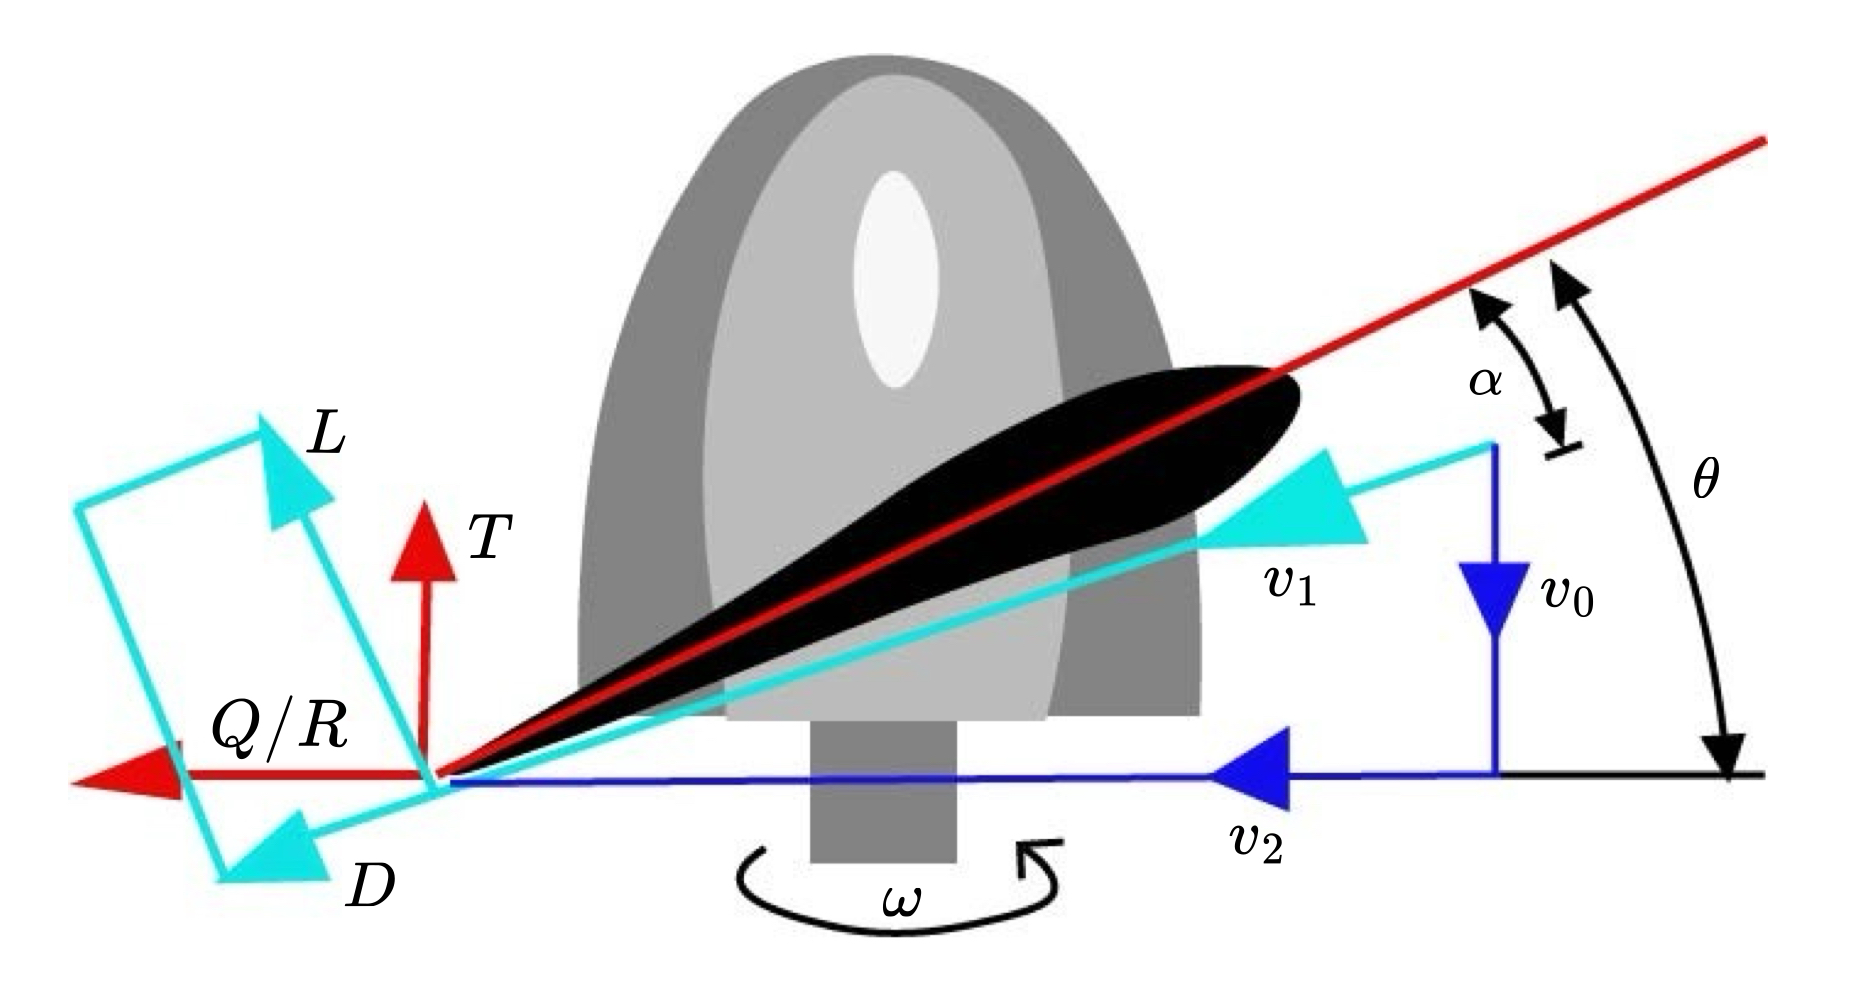
\includegraphics[width=0.5\textwidth]{aeroforces.jpg}}
\caption{Aerodynamic Analysis of Blade Element}
\label{fig:aeroforce}
\end{figure}
\begin{figure}[htbp]
    \centering
    \begin{subfigure}[b]{0.45\textwidth}
        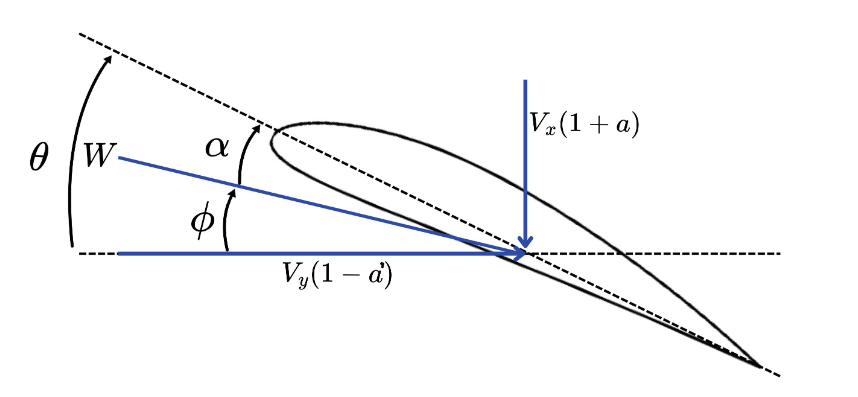
\includegraphics[width=\textwidth]{geomBEMT.png}
        \caption{Aeromechanical Analysis of Blade Element under Classical BEMT }
        \label{fig:graph1}
    \end{subfigure}
    \hfill
    \begin{subfigure}[b]{0.45\textwidth}
        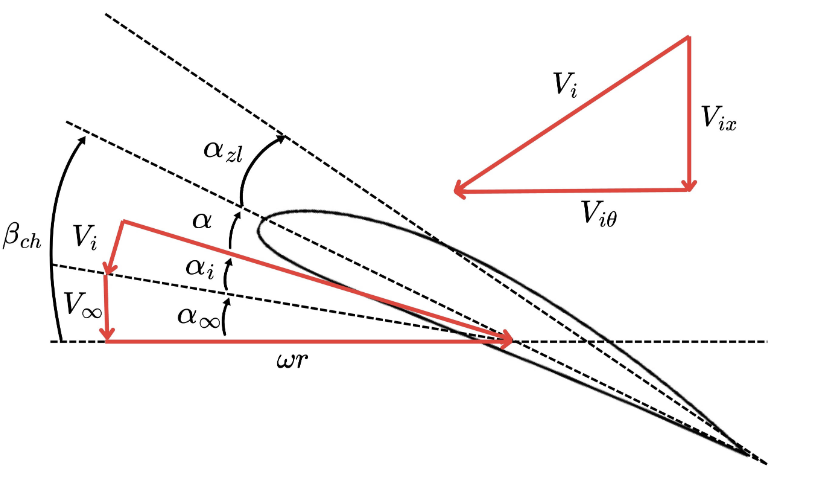
\includegraphics[width=\textwidth]{geomTRAUBS.png}
        \caption{Aeromechanical Analysis of Blade Element under Traub's Theory (Modified BEMT)}
        \label{fig:graph2}
    \end{subfigure}
    \caption{Comparative Aeromechanical Analysis of Blade Elements: Classical BEMT vs. Traub's Modified BEMT.}
    \label{fig:comparison}
\end{figure}


Having established the foundational principles of BEMT, the mathematical formulation that underpins the classical theory is based on the development of linear and angular momentum conservation which leads to a set of differential equations that describe the thrust and torque generated by the propeller. These equations are iteratively solved to predict the aerodynamic performance of the entire propeller, derived by considering both the axial and tangential components of the induced velocity as the air passes through the rotor disk. The disk, in this context, can be seen as a Gaussian surface that describes the propeller's effective interaction with the airflow, capturing the induced velocities and the aerodynamic forces acting on each blade element.

In BEMT, \cite{ning2021} explains that induced velocities are characterized by two critical factors: the axial induction factor \( a \) and the tangential induction factor \( a' \). These factors allow the determination of the differential thrust \( dT \) and differential torque \( dQ \) generated by a blade element at a radial position \( r \), and how they are influenced by the reduction in axial velocity across the rotor disk. In this context, \( \rho \) represents the air density, which affects the generated thrust and torque as it determines the amount of air mass interacting with the propeller, while \( V_\infty \) denotes the free-stream air velocity (or "advance speed" of the aircraft), which is the axial component of the airflow interacting with the propeller before being influenced by the rotation of the blades.

The differential thrust \( dT \) generated by a blade element is given by:
\begin{equation}
dT = 4 \pi r \rho V_{\infty} (1 - a) v_{\text{ind}} \, dr
\end{equation}
where \( v_{\text{ind}} = a V_{\infty} \) represents the induced axial velocity.

Similarly, the differential torque \( dQ \) produced by the same blade element, which depends on the tangential component of the airflow, the induced tangential velocity \( v_{\theta} \), is given by:
\begin{equation}
dQ = 4 \pi r^3 \rho V_{\infty} (1 - a') v_{\theta} \, dr
\end{equation}
Here, \( v_{\theta} = a' r \Omega \) is the induced tangential velocity, related to the rotational speed of the rotor \( \Omega \).

The solution for \(a\) and \(a'\), variables that require an iterative approach, following the algorithms and explanations developed by \cite{ning2021}. Both factors depend on the flow conditions and the aerodynamic forces acting on the blade elements. Initially, estimated values of \(a\) and \(a'\) are used to compute the relative velocity \(v_{\text{rel}}\), which is the velocity experienced by the blade element:
\begin{equation}
v_{\text{rel}} = \sqrt{(v_{\infty} (1 - a))^2 + (r \Omega (1 + a'))^2}
\end{equation}
This relative velocity allows for the determination of the flow angle \(\phi\), the angle of attack \(\alpha\), the twist angle \(\theta\). (Note that the twist angle is a combination of the geometric angle $\alpha_{geom}$, or default blade angle, and the propeller pitch applied at the hub $\beta$) :
\begin{equation}
    \phi = \tan^{-1} \left( \frac{v_{\infty} (1 - a)}{r \Omega (1 + a')} \right)
\end{equation}
\begin{equation}
    \alpha = \theta - \phi
 \end{equation}
 \begin{equation}
    \theta = \alpha_{geom} + \beta
 \end{equation}
Using the angle of attack \(\alpha\), the coefficients of lift \(C_L\) and drag \(C_D\) are obtained from airfoil data for the blade section, where \( c \) represents the chord length of the blade section. These coefficients enable the calculation of the aerodynamic forces:
\begin{equation}
    dL = \frac{1}{2} c \rho v_{\text{rel}}^2 C_L \, dr
\end{equation}
\begin{equation}
    dD = \frac{1}{2} c \rho v_{\text{rel}}^2 C_D \, dr
\end{equation}

Subsequently, updated values for \(a\) and \(a'\) are computed using:
\begin{equation}
    a = \frac{1}{1 + \frac{4 \sin^2 \phi}{\sigma C_L}} \ \  \ \ 
\end{equation}
\begin{equation}
    a' = \frac{1}{1 + \frac{4 \sin \phi \cos \phi}{\sigma C_D}}
\end{equation}
This process is repeated until the values of \(a\) and \(a'\) converge, ensuring that the momentum and blade element theories are in equilibrium. Once the induction factors have converged, \cite{ning2021} explain that the total thrust \(T\) and torque \(Q\) can be determined by integrating the differential contributions from each blade element over the entire span of the rotor:
\begin{equation}
T = \int_{r_{\text{hub}}}^{r_{\text{tip}}} 4 \pi r \rho v_{\infty} (1 - a) v_{\text{ind}} dr 
\end{equation}
\begin{equation}
Q = \int_{r_{\text{hub}}}^{r_{\text{tip}}} 4 \pi r^3 \rho v_{\infty} (1 - a') v_{\theta} dr
\end{equation}
These integrals are usually evaluated using numerical methods,  such as Newton-Cotes or Gaussian quadrature, to obtain the total of these variables produced by the propeller operation.

However, although widely used for propeller analysis, it presents several limitations that must be considered. First, the inherent limitation of BEMT and its derivatives is that the accuracy of the method largely depends on the radial discretization of the blade, which can lead to errors if an insufficient number of discretized stations are used along the radius. Additionally, the second and more significant limitation is the estimation of axial and tangential induction factors, which represent the effects of the helical wake and require an iterative process that can introduce uncertainty into the results. Another important aspect is the reliance on extensive aerodynamic databases, which necessitates the use of lookup tables to obtain lift and drag coefficients based on the angle of attack and the Reynolds number, limiting the model's flexibility. Furthermore, accurately modeling the stall phenomenon at low advance ratios is challenging due to rotational effects, such as the Coriolis contribution and radial pressure gradients, which can compromise performance predictions under separated flow conditions.

For this reason, the analysis of the propeller was based on \cite{traub2016}, which develops a theory derived from BEM but takes its limitations into account and contributes to improving the method. Unlike BEM, Traub's theory can be applied to dynamic systems, not just stationary ones, making it ideal for aircraft characterization.

\subsubsection{Traub's Theory (BEMT dynamic derivation)}

Considering the points mentioned above, in order to perform a correct analysis of propellers, it is necessary to move away from the static perspective we used with BEMT. As \cite{ning2021} points out, that integral averaging method only works well for wind turbines due to their large size, which limits its application when attempting to design aircraft propellers. Due to this, the propeller analysis was based on \cite{traub2016}, which develops a theory derived from BEM but takes its limitations into account and contributes to improving the method. Unlike BEM, Traub’s theory can be applied to dynamic systems, not just stationary ones, where changing conditions, velocities, or both play an important role in how the system reacts. 

So, \cite{traub2016} proposed a non-iterative propeller analysis method that is easy to implement and suitable for design purposes. It incorporates a stall model and aerofoil data approximation, reducing the reliance on look-up tables for aerofoil characteristics. The method, based on vortex theory by Phillips, accounts for Reynolds number and angle-of-attack effects, and is optimized for use in spreadsheet programs. The approach recalculates the lift and drag coefficients using experimental databases, thereby estimating the stall phenomenon more accurately.

The steps comprising this model, as applied here, are presented below according to \cite{traub2016}:
\begin{enumerate}
    \item Discretize the blade from the hub at \( r/R = 0.05, 0.1, \dots \) up to \( r/R \approx 0.95 \) to model the blade accurately. Calculations will be done at each \( r \).
    
    \item If the blade is variable pitch, the pitch angle can be added to the local blade pitch \( \beta_{\text{ch}}(r) \) for all $r$. The definition of pitch described here differs from that in BEMT, where pitch is a component of the twist angle rather the twist angle itself.  

    \begin{equation}
        \alpha = \beta_{\text{ch}} - \alpha_i - \alpha_{\infty}.
    \end{equation}
    
    Here, \(\alpha_i\) and \(\alpha_{\infty}\) are equivalent to the inflow angle \(\phi\) in the classical BEMT, variables which will developed in the following steps.
    
    \item Calculate the tip loss factor \( F(r) \):
    \begin{equation}\label{eq:tip_loss}
        F(r) = \frac{2}{\pi} \cos^{-1} \left( e^{\frac{-B(1 - r/R)}{2 \sin \beta_{\text{tip}}}} \right)
    \end{equation}
    where, \( \beta_{tip} \) is the inflow angle at the radial position \( r \)
    
    \item Determine the flow angle \(\alpha_{\infty}(r)\), excluding induced effects:
    \begin{equation}
        \alpha_{\infty}(r) = \tan^{-1}\left( \frac{V_{\infty}}{\omega r} \right)
    \end{equation}

    \item Calculate the induced angle-of-attack \(\alpha_i(r)\) using constants \(A(r)\), \(B(r)\), and \(C(r)\):
    \begin{equation}
        \begin{aligned}
            A(r) &= F(r) \frac{\pi}{2} \cos(\alpha_{\infty}(r)), \quad B(r) = \frac{Bc(r)}{16r} c_{l\alpha}(r) + F(r) \frac{\pi}{2} \sin(\alpha_{\infty}(r)), \\
            C(r) &= -\frac{Bc(r)}{16r} c_{l\alpha}(r) [\beta_{\text{ch}}(r) - \alpha_{\infty}(r) - \alpha_{z}], \\
            \alpha_i(r) &= \frac{-B(r) + \sqrt{B(r)^2 - 4A(r)C(r)}}{2A(r)}
        \end{aligned}
    \end{equation}
    
    \item Calculate \(X(r)\) to use later in the lift \(c_l(r)\) and drag coefficients \(c_d(r)\):
    \begin{equation}
        X(r) = \frac{1}{1 + e^{\sigma [\alpha(r) - \alpha_{\text{stall}}]}}
    \end{equation}
    \item Calculate the local lift coefficient, \( c_l(r) \) (\autoref{fig:Traub}).
    \item (Optional)* Calculate the local Reynolds number \( Re(r) \) only if \( c_{d_{\text{min}}}(r) \approx A Re(r)^{\gamma} \):
    \begin{equation}
        Re(r) = \frac{\omega r \cos(\alpha_i(r)) \rho c(r)}{\cos(\alpha_{\infty}(r)) \mu}
    \end{equation}
    Otherwise, use XFOIL to determine \( c_{d_{\text{min}}} \).
    
    \item Calculate the local drag coefficient, \( c_d(r) \) (\autoref{fig:Traub}) .
    
    \item Evaluate and integrate to find the Thrust  (\(T\)) and Torque (\(Q\)), following Traub equations (\autoref{fig:Traub}).
\end{enumerate}


% The steps that develop this model and will be applied here are presented below, according to \cite{traub2016}:
% \begin{enumerate}
%     \item Discretise the blade, starting at the hub, or \( r/R = 0.05, 0.1 \) to no less than \( 0.95R \) (to model the blade as completely as possible). The equations are evaluated at each \( r \).
    
%     \item If the blade is variable pitch, the pitch angle can be added to the local blade pitch \( \beta_{\text{ch}}(r) \) for all \( r \). The definition of pitch described here differs from that in BEMT, where pitch is a component of the twist angle rather than the twist angle itself.
%     \begin{equation}
%         \alpha = \beta_{\text{ch}} - \alpha_i - \alpha_{\infty}.
%     \end{equation}
%    Here, \(\alpha_i\) and \(\alpha_{\infty}\) are equivalent to the inflow angle \(\phi\) in classical BEMT, variables which will be developed in the following steps.
%     \item Calculate the tip loss factor, \( F(r) \):
%     \begin{equation}\label{eq:tip_loss}
%         F(r) = \frac{2}{\pi} \cos^{-1} \left( e^{\frac{-B(1 - r/R)}{2 \sin \beta_{\text{tip}}}} \right)
%     \end{equation}
%     \item Calculate the angle of the resulting flow excluding induced effects, \( \alpha_{\infty}(r) \):
%     \begin{equation}
%         \alpha_{\infty}(r) = \tan^{-1}\left( \frac{V_{\infty}}{\omega r} \right)
%     \end{equation}
%     \item Calculate the induced angle-of-attack, \( \alpha_i(r) \):
%     \begin{equation}
%         \begin{aligned}
%         A(r) &= F(r) \frac{\pi}{2} \cos(\alpha_{\infty}(r)) \\
%         B(r) &= \frac{Bc(r)}{16r} c_{l\alpha}(r) + F(r) \frac{\pi}{2} \sin(\alpha_{\infty}(r)) \\
%         C(r) &= -\frac{Bc(r)}{16r} c_{l\alpha}(r) [\beta_{\text{ch}}(r) - \alpha_{\infty}(r) - \alpha_{z}]
%         \end{aligned}
%     \end{equation}
%     where:
%     \begin{equation}
%         \alpha_i(r) = \frac{-B(r) + \sqrt{B(r)^2 - 4A(r)C(r)}}{2A(r)}
%     \end{equation}
%     \item Calculate \( X(r) \), Equation (12), and then the local lift coefficient, \( c_l(r) \):
%     \begin{equation}
%         X(r) = \frac{1}{1 + e^{\sigma [\alpha(r) - \alpha_{\text{stall}}]}}
%         \end{equation}
%     \begin{equation}
%         c_l(r) = c_{l\alpha}(r) \left[\beta_{\text{ch}}(r) - \alpha_z - \alpha_i(r) - \alpha_{\infty}(r) \right] \left[ \frac{1 + X(r)^m}{2} \right]^2
%         \end{equation}
%     \item Calculate the local Reynolds number:
%     \begin{equation}
%         Re(r) = \frac{\omega r \cos(\alpha_i(r)) \rho c(r)}{\cos(\alpha_{\infty}(r)) \mu}
%         \end{equation}
%     \item Calculate the local drag coefficient, \( c_d(r) \):
%     \begin{equation}
%         c_d(r) = X(r) [c_{d_{min}}(r) + k_p (c_l(r) - c_{lmd})^2] + (1 - X(r)) [c_{l}(r) \tan(\alpha(r)) + 0.5c_{d_{\text{min}}}(r) \cos(\alpha_{\text{geom}}(r))]
%     \end{equation}
%     \item Evaluate and integrate to find the Thrust and Torque:
%     \begin{equation}
%     T = \frac{B \rho \omega^2}{2} \int_{r=\text{hub}}^R \frac{r^2 c(r) \cos^2(\alpha_i(r))}{\cos^2(\alpha_{\infty}(r))} c_l(r) 
%     \left[ \cos(\alpha_i(r) + \alpha_{\infty}(r)) - \frac{c_d(r)}{c_l(r)} \sin(\alpha_i(r) + \alpha_{\infty}(r)) \right] dr
%     \end{equation}
%     \begin{equation}
%     Q = \frac{B \rho \omega^2}{2} \int_{r=\text{hub}}^R \frac{r^3 c(r) \cos^2(\alpha_i(r))}{\cos^2(\alpha_{\infty}(r))} c_l(r)
%     \left[ \sin(\alpha_i(r) + \alpha_{\infty}(r)) + \frac{c_d(r)}{c_l(r)} \cos(\alpha_i(r) + \alpha_{\infty}(r)) \right] dr
%     \end{equation}
% \end{enumerate}

After presenting Traub's algorithm, its model block would be structured as presented in \autoref{fig:Traub}.

\begin{figure}[H]
    \hspace{-2cm}
    \begin{tikzpicture}
        % Definir estilos
        \tikzstyle{block} = [draw, fill=Goldenrod!30, rectangle, minimum height=13em, minimum width=10em, text centered, text width=2.2cm, rounded corners]
        \tikzstyle{block_1} = [draw, fill=NavyBlue!30, rectangle, minimum height=5em, minimum width=10em, text centered, text width=2.2cm, rounded corners]
        \tikzstyle{model} = [draw, fill=white!20, rectangle, minimum height=2.5em, minimum width=26em, text centered, text width=10.2cm]
        \tikzstyle{input} = [node distance=-1.5cm, text centered]
        \tikzstyle{output} = [node distance=2cm, text centered]
        \tikzstyle{cloud} = [draw, ellipse,fill=white!20, node distance=3cm, minimum height=2em]
        \tikzstyle{line} = [draw, -latex']
        
        %\draw[dashed] (-10,0) rectangle (-1,8);
        
        \draw [dashed] (1.3,-0.5) node[minimum height=7.1cm,minimum width=14.8cm,draw];
               
        % Fondo amarillo
        %\filldraw [fill=black!20, draw=none] (0,0) rectangle (10,5);
        \draw (1.3,-0.5) node[fill=black!20, minimum height=7cm,minimum width=14.7cm,draw=none];
        
        
        % Etiqueta del modelo 
        \node at (7,2.5) {Traubs Model};
        %at (-10.6,0)


        
        % Bloque de cálculos
        \node [block] (calc) at (-4.1,0.1){Calculations:\\ $\rho^{i},\mu^{i},\alpha_{\infty}, \alpha_{ind}, \\ \alpha(r), Re(r)^{*}, X(r)$ \\Parameters: $\sigma, m$\\ Geometry:\\B, R, $\alpha_{geom}, \alpha_{zl}$};

         %Bloque XFOIL
        \node [block_1] (xfoil) at (-4.1,-2.6){XFOIL: $C_{lmd}, C_{dmin}, C_{l\alpha},\\ $K_p$, \alpha_{stall}$};

        % Entrada de flujo masico
        \node (flux)at (-7.5,0.9){$V_{\infty}$};
        \node [below of=flux, node distance=-0.4cm](flux_text) {Air Velocity};
        \draw [->, -latex] (flux.east) -- ([yshift=0.8cm] calc.west);

        % Entrada de velocidad
        \node [input, below of=flux, node distance=0.8cm] (vel){$\omega$};
        \node [below of=vel, node distance=-0.4cm](vel_text) {Angular Velocity };
        \draw [->, -latex] (vel.east) -- ([yshift=0cm] calc.west);

        % Entrada de presión
        \node [input, below of=vel, node distance=0.8cm] (pressure) {$\beta_{ch}$};
        \node [below of=pressure, node distance=-0.4cm] (pressure_text) {Pitch Angle};
        \draw [->, -latex] (pressure.east) -- ([yshift=-0.8cm]calc.west);

        % Caja de salida de CL
        \node [model] (potencia_out) at (3.3,1.7) {$C_{l}(r) = C_{l\alpha}[\beta_{ch}(r) - \alpha_{zl}(r)-\alpha_{ind}(r)-\alpha_{\infty}(r)][\frac{1+X(r)^{m}}{2}]^{2}$};
        \draw [->, -latex] (calc.east) -- (potencia_out.west);
            
        % Caja de salida de CD
        \node [model, below of=potencia_out, node distance=1.08cm] (temp_out){$C_{d}=X(r)[C_{dmin}(r)+K_p(C_{l}(r)-C_{lmd})^{2}]$\\ $+(1-X(r))[C_{l}(r)tan(\alpha(r))+0.5C_{dmin}(r)cos(\alpha_{geom}(r))]$};       
        \draw [->, -latex] (calc.east) -- (temp_out.west);
        
        % Caja de salida de THRUST
        \node [model,  below of=temp_out, node distance=2.31cm] (pressure_out) {$T = \frac{B\rho^{i}\omega^{2}}{2}\int_{r_{hub}}^{R}r^2c(r)\frac{cos^{2}(\alpha_{ind}(r))}{cos^{2}(\alpha_{\infty}(r))}C_{l}(r)\\ \times(cos[\alpha_{ind}(r)+\alpha_{\infty}(r)]-\frac{C_{d}(r)}{C_{l}(r)}sin[\alpha_{ind}(r)+\alpha_{\infty}(r)])dr$};
        \draw [->, -latex] (calc.east) -- (pressure_out.west);
        \draw [->, -latex] ([xshift=-3.8cm]temp_out.south) -- ([xshift=-3.8cm]pressure_out.north);
        \node (potencia)at(0.8,-0.7){$C_{l}$};
        \node [below of=potencia, node distance=-0.4cm](potencia_text) {Lift Coefficient};


        \draw [->, -latex] ([xshift=1.1cm]temp_out.south) -- ([xshift=1.1cm]pressure_out.north);
        \node (temp)at(5.8,-0.7){$C_{d}$};
        \node [below of=temp, node distance=-0.4cm](temp_text) {Drag Coefficient};


        % Caja de salida de TORQUE
        \node [model,  below of=pressure_out, node distance=1.48cm] (torque_out) {$Q = \frac{B\rho^{i}\omega^{2}}{2}\int_{r_{hub}}^{R}r^3c(r)\frac{cos^{2}(\alpha_{ind}(r))}{cos^{2}(\alpha_{\infty}(r))}C_{l}(r)\\ \times(sin[\alpha_{ind}(r)+\alpha_{\infty}(r)]+\frac{C_{d}(r)}{C_{l}(r)}cos[\alpha_{ind}(r)+\alpha_{\infty}(r)])dr$};
        \draw [->, -latex] (calc.east) -- (torque_out.west);

        % Etiquetas de salida
        %\node (potencia)at(10.5,0.7){$C_{l}$};
        %\node [below of=potencia, node distance=-0.4cm](potencia_text) {Lift Coefficient};
        %\draw [->, -latex] (potencia_out.east) -- (potencia.west);

        %\node [input, below of=potencia, node distance=1.07cm](temp){$C_{d}$};
        %\node [below of=temp, node distance=-0.4cm](temp_text) {Drag Coefficient};
        %\draw [->, -latex] (temp_out.east) -- (temp.west);
        
        \node (pressure)at(10,-1.7){$T$};
        \node [below of=pressure, node distance=-0.4cm](pressure_text) {Thrust};
        \draw [->, -latex] (pressure_out.east) -- (pressure.west);

        \node [input, below of=pressure, node distance=1.47cm](torque){$Q$};
        \node [below of=torque, node distance=-0.4cm](torque_text) {Torque};
        \draw [->, -latex] (torque_out.east) -- (torque.west);
    \end{tikzpicture}
    \caption{Traub BEMT Model}
    \label{fig:Traub}
\end{figure}

To obtain more precise values that characterize the behavior of the blades, correction factors have been implemented to adjust certain aerodynamic parameters. In fact, Traub's contemplates two important phenomena: Tip losses and Boundary Layer Compressibility - Stall angle.

Taking into account the above, one of the most widely used is the Prandtl Tip Loss Factor \( F \), which provides a more realistic representation of thrust and torque generated along the entire propeller. As mentioned in \cite{burton2011wind}, this factor is critical in the analysis of propellers and turbines, as tip losses limit the efficiency of the propulsion system, especially under high-speed or high-load conditions. 

The tip loss factor is defined as a correction to account for efficiency losses at the blade tips, which occur due to vortex formation. By applying Prandtl’s correction in the BEMT, thrust and torque calculations are adjusted to reflect the reduced contribution from the tips, providing a more accurate estimate of the overall performance of the propeller. As evidenced in \cite{traub2016}, the use of tip loss correction becomes a fundamental part of the method, enabling more precise and reliable results in propeller performance analysis. Prandtl’s formulation is expressed in equation (\ref{eq:tip_loss}), this factor \( F \) adjusts the thrust and torque calculations to better reflect the reduced contribution from the blade tips.

On the other hand, Stall in the blades of a propeller following theory on \cite{burton2011wind} occurs when the angle of attack exceeds a critical limit, leading to an abrupt decrease in the lift coefficient and, consequently, reducing the efficiency of the blade in generating thrust. This phenomenon arises when the airflow no longer adheres to the blade surface due to an increase in pressure on the blade’s rear surface, causing what is known as boundary layer separation. When stall occurs, zones of recirculation or separation bubbles form on the blade’s surface, increasing aerodynamic drag and generating unwanted vibrations in the propeller. This effect significantly impacts propeller efficiency, particularly at high speeds and elevated angles of attack, and can also affect aircraft stability by increasing the structural load on the blades.

Incorporating these correction factors, Traub’s algorithm enhances the precision of propeller performance analysis. By refining thrust and torque estimations and accounting for stall effects, this approach enables a more reliable and accurate representation of the propeller’s behavior across diverse flight conditions.

\subsection{Operative Conditions}
This section presents the models incorporated to simulate real-flight phenomena, including air conditions, fuel injection, aircraft speed, and torque control. These models allow the simulation to capture key altitude-dependent variations in atmospheric conditions, optimize fuel delivery for each flight phase, and test a realistic range of operational speeds. Additionally, a PID control system continuously adjusts the propeller pitch, maintaining required torque and stability across different flight stages. Together, these elements provide a comprehensive framework for evaluating turboprop performance in realistic conditions.


\subsubsection{Atmospheric Modeling}
    To analyze how the initial atmospheric parameters, such as atmospheric pressure, temperature, air density, and viscosity, vary, existing literature was consulted to find the relationships between these parameters. It was found that altitude affects each of them differently, according to equations described in the theory developed by \cite{us_standard_atmosphere_1976}, which characterizes the behavior of the atmosphere under different altitude gradients. The following section presents the formulation used, based on \cite{us_standard_atmosphere_1976}, to model these variable gradients. 
    
    \begin{enumerate} [label=\alph*)]

    \item \textbf{Temperature in the Troposphere}
    \\
    The temperature variation with altitude is linear in the troposphere and can be expressed as:
    
    \begin{equation}\label{eq:temp}
       T(h) = T_0 - Lh  
    \end{equation}
    
    where \( T_0 \) represents the temperature at sea level and \( L \) is the temperature lapse rate, indicating how much the temperature decreases per meter of altitude. 
    
    \item \textbf{Atmospheric Pressure}
    \\
    The atmospheric pressure decreases with altitude according to the following relation:
    
    \begin{equation}\label{eq:pressure}
            P(h) = P_0 \left( \frac{T(h)}{T_0} \right)^{\frac{g}{LR}}
    \end{equation}
    
    In this equation, \( P_0 \) is the pressure at sea level and The constant \( g \) stands for the gravitational acceleration.
    
    \item \textbf {Air Density}
    \\
    The altitude-dependent air density can be calculated using the ideal gas law:
    
    \begin{equation}\label{eq:density}
        \rho(h) = \frac{P(h)}{RT(h)}
    \end{equation}
    
    \item \textbf {Air Viscosity (Sutherland's Law)}
    \\
    The dynamic viscosity of air changes with temperature, and is described by Sutherland's law:
    \\
    \begin{equation}\label{eq:viscosity}
        \mu(T) = \mu_0 \frac{T_0 + C}{T + C} \left( \frac{T}{T_0} \right)^{3/2}        
    \end{equation}

    In this formula, \( \mu(T) \) represents the dynamic viscosity at a given temperature \( T \), with \( \mu_0 \) as the reference viscosity at the reference temperature \( T_0 \). The constant \( C \) is Sutherland's constant, specific to the gas being analyzed (Air).
    
    \end{enumerate}
    
\subsubsection{Fuel Control}
    Before the engine can sustain its own operation, it must reach certain initial parameters through a “pre-start” process. For this, an external power source, such as a battery, is needed to turn the gas generation shaft and achieve the minimum operating conditions required to initiate fuel injection.
    
    Fuel control is a crucial element in the efficient operation of a turboprop engine, as it ensures precise fuel mass flow delivery during each flight phase, optimizing engine performance and preventing unwanted fluctuations. For the PT6A  engine and McCauley propeller, a control system was implemented that adjusts the fuel flow according to the specific requirements explained by \cite{vecchiio2024} of each stage, from start-up to landing, ensuring stability and efficiency throughout the flight.

\subsubsection{Aircraft Speed}
The developed simulation focuses on the behavior of the turboprop engine and propeller under various operational conditions, excluding the complete aerodynamic structure of the aircraft (fuselage, wings, etc.). This approach limits our ability to precisely model how thrust translates into aircraft speed, as essential aerodynamic factors are not represented. Consequently, the thrust calculated using Traub’s theory \cite{traub2016} does not account for the aircraft’s total drag, a crucial factor in determining maximum achievable speed.

Rather than setting a fixed limit for maximum speed, we tested a range of velocities, starting from 80 km/h and progressively increasing. At speeds between 120 and 130 knots (approximately 240 km/h), general aviation aircraft such as the Cessna 172 Skyhawk \cite{cessna_skyhawk_2024}, Piper PA-28 Cherokee \cite{piper_cherokee_2021}, and Diamond DA-20 \cite{diamond_da20_2024} were considered, as they are designed to operate within this velocity range. As the speeds increased further, we aligned with turboprop aircraft like the Air Tractor AT-602, AT-802 \cite{airtractor6022024,airtractor802a2024}, and the Thrush 710P \cite{thrush710p2024}, which typically reach speeds around 350 km/h. Extending the range even higher, we approached the velocities of more aerodynamically optimized models, including the Pilatus PC-12 \cite{pilatus2016} and Piper Cheyenne IIIA \cite{piper2016}, where speeds can range between 500 and 600 km/h.

Hence, different evalutions were performed to a broad range of speeds to assess the simulation’s consistency across multiple values, identifying the limits within which the model’s results align with realistic aerodynamic performance.

\subsubsection{PID control}
    The analysis of torque and angular velocity of the propeller is crucial to meet the requirements of each flight phase by adjusting these parameters through the pitch angle ($\beta_{ch} $), which controls the amount of air passing through the propeller and prevents overloads. To ensure that the torque remains within optimal pre-established values for each flight stage according to \cite{Castellanos2023Propeller}, a PID controller is implemented. This controller, through constant comparison between $\tau_{nom}$ and $\tau_{real}$ (calculated based on Traub's theory), adjusts the pitch angle. This adjustment is made through a feedback loop in which the PID reduces the error to zero in relation to the specific torque values for each phase (\autoref{fig:PitchPID}), adjusting the proportional ($K_p$), integral ($K_i$), and derivative ($K_d$) constants. Thus, the system adapts in real time, maintaining the stability and safety of the aircraft during all phases of flight.   
    \begin{figure}[H]
    \centering
    {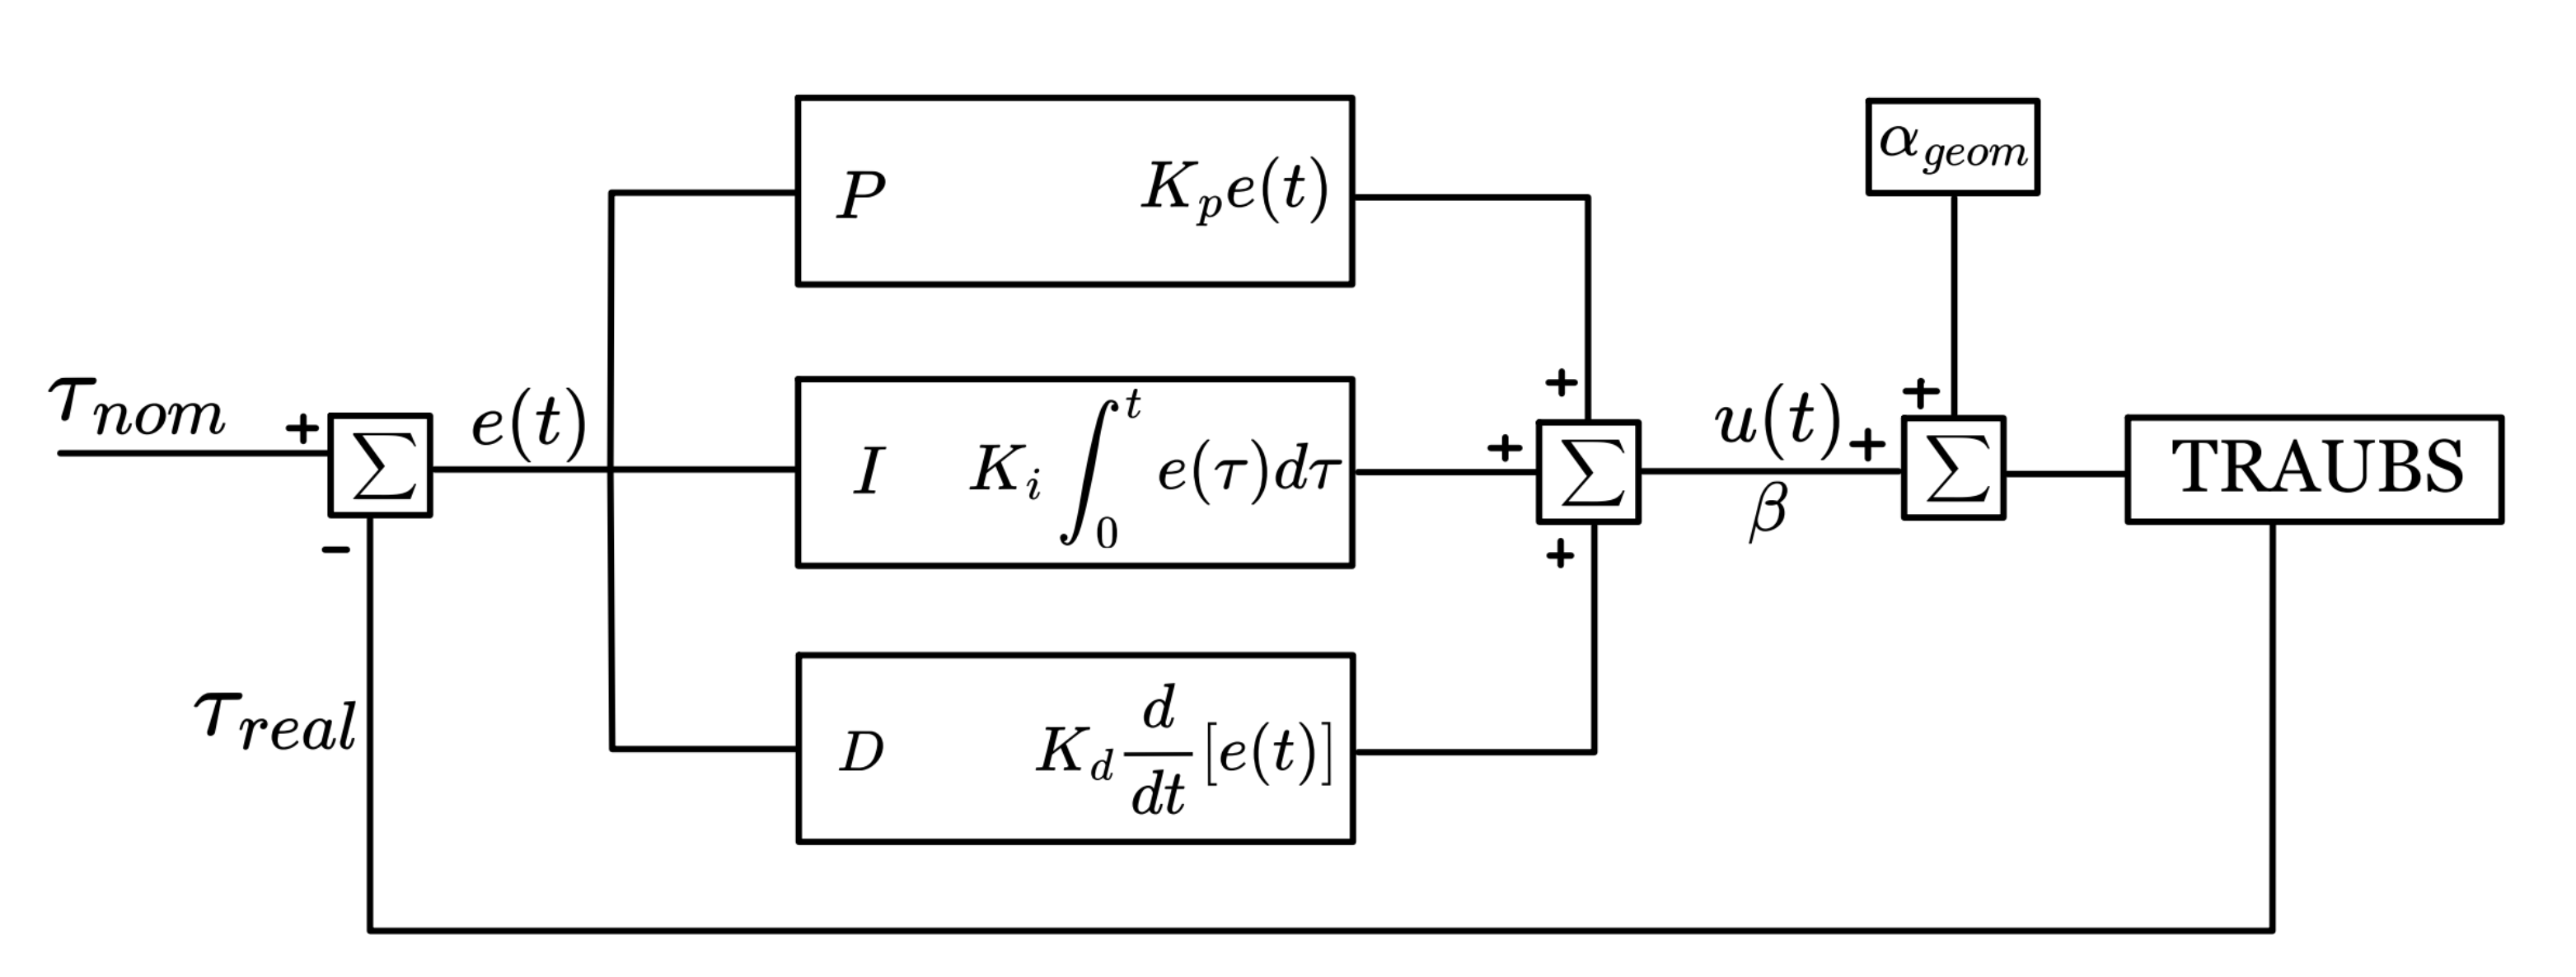
\includegraphics[width=0.60\textwidth]{pid_controller.png}}
    \caption{Pitch Angle PID control}
    \label{fig:PitchPID}
    \end{figure}

\section{Codification Section: \emph{To code a modular computational tool in Matlab-Simulink that numerically solves the formulation from objective 1}}\label{sec:Method}

A nonlinear dynamic system was identified, which is why Simulink was used, employing the numerical method of fourth-order Runge-Kutta. This method is used to solve the set of differential equations, including nonlinear equations, corresponding to the mathematical models presented previously. A complete engine-propeller system model was implemented in Simulink, as evidenced in (\autoref{fig:simulink}), with MATLAB arrays representing the general geometries of both components. The engine simulation was structured into three main sections: compressors (\autoref{fig:Inlet} to \autoref{fig:Centcomp}), combustion (\autoref{fig:CombChamber}), and turbines (\autoref{fig:Turbine}). The power output from turbines 2 and 3 was directed to the power shaft, which was connected to the propeller. The propeller section was divided into two parts: a Simulink block coded based on the TRAUB model as appears in \autoref{fig:Traub}, which received the pitch angle, free stream velocity, and RPM as inputs, inside, thrust and torque were calculated at each instant using coefficients derived from Excel functions according to TRAUB theory. The torque output was connected to a PID controller, that allowed adjust the propeller’s pitch angle as shown in \autoref{fig:PitchPID} in each operational phase, ensuring an appropriate response across various flight conditions.

\begin{figure}[H]
    \centering
    {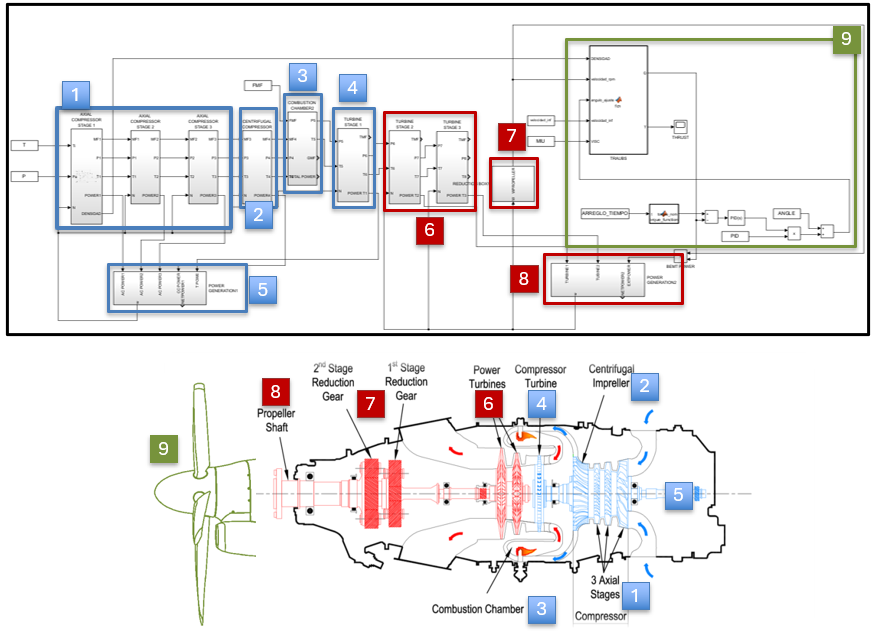
\includegraphics[width=0.80\textwidth]{simulink_diagrama.png}}
    \caption{Simulink Diagram vs Turboprop}
    \label{fig:simulink}
\end{figure}

\subsection{XFOIL - Traub: Computational Implementation}
In \autoref{fig:Cdmin}, \ref{fig:Clmd} and \ref{fig:kp}, it can be seen the graphs made from the Excel document and the behavior of $c_{lmd}$, $c_{d_{min}}$, and $k_p$ along the radius of the blade. Finally, Algorithm \ref{alg:torque_thrust_calculation} demonstrates Traub's procedure for calculating torque and thrust, utilizing the previously determined variables.
\begin{figure}[h]
    \centering
    \begin{subfigure}[b]{0.39\textwidth}
    {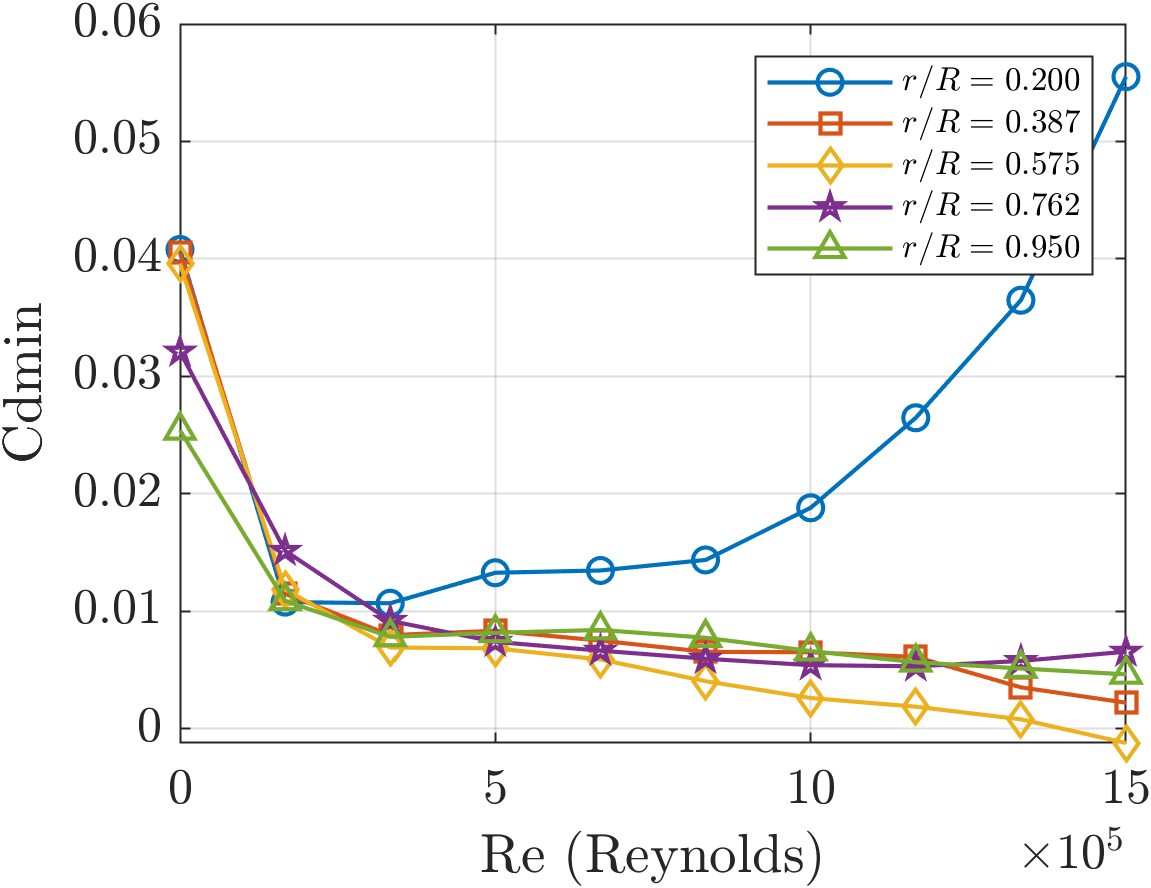
\includegraphics[width=\textwidth]{Cdmin_2D.png}}
    \caption{Graph 1: Relationship between $C_{dmin}$ and $Re$ along the blade}
    \label{fig:Cdmin}
    \end{subfigure}
    \hspace{0.02\textwidth}
    \begin{subfigure}[b]{0.39\textwidth}
        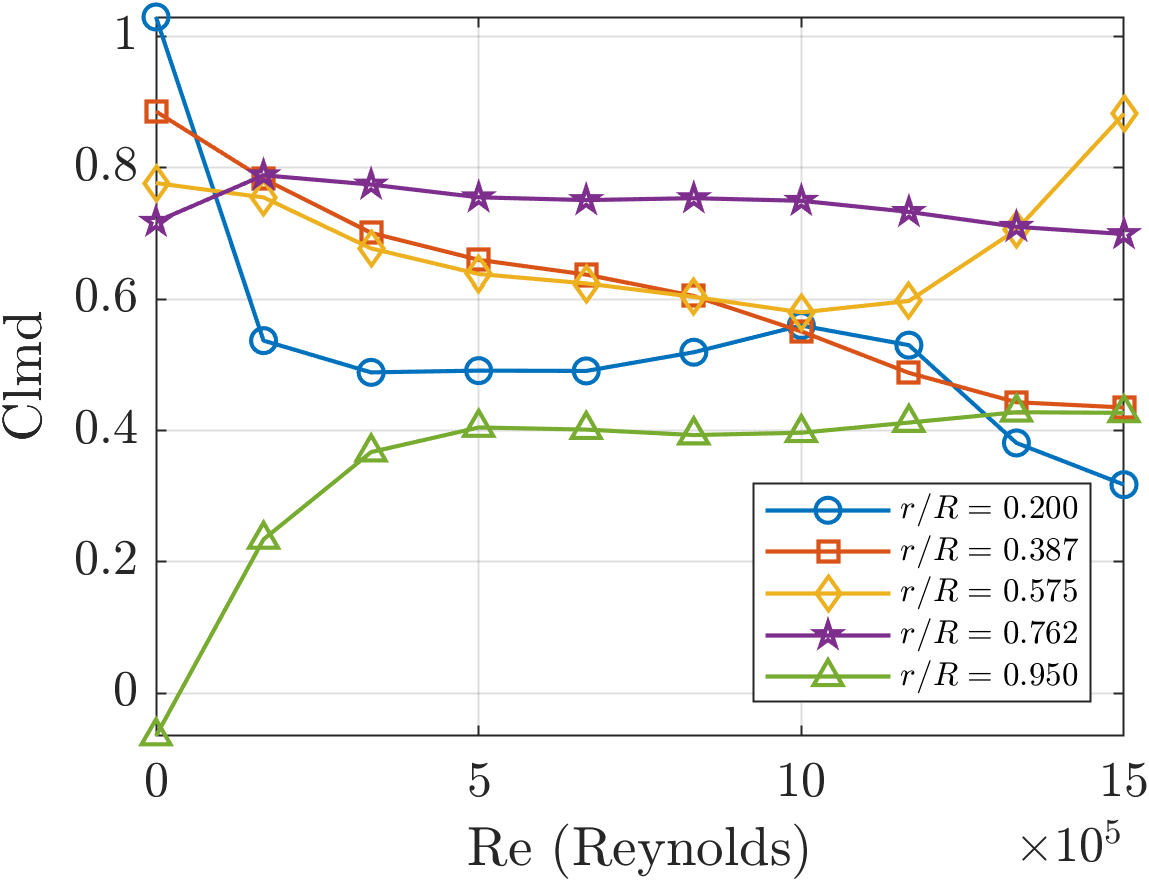
\includegraphics[width=\textwidth]{Clmd_2D.png}
        \caption{Graph 2: Relationship between $C_{lmd}$ and $Re$ along the blade}
        \label{fig:Clmd}
    \end{subfigure}
    \vskip\baselineskip
    \caption{Relationship between $C_{dmin}$ and $C_{lmd}$ against $Re$ along the blade}
    \label{fig:Relationship_Kp_Clmd}
\end{figure}

\begin{figure}[H]
    \centering
    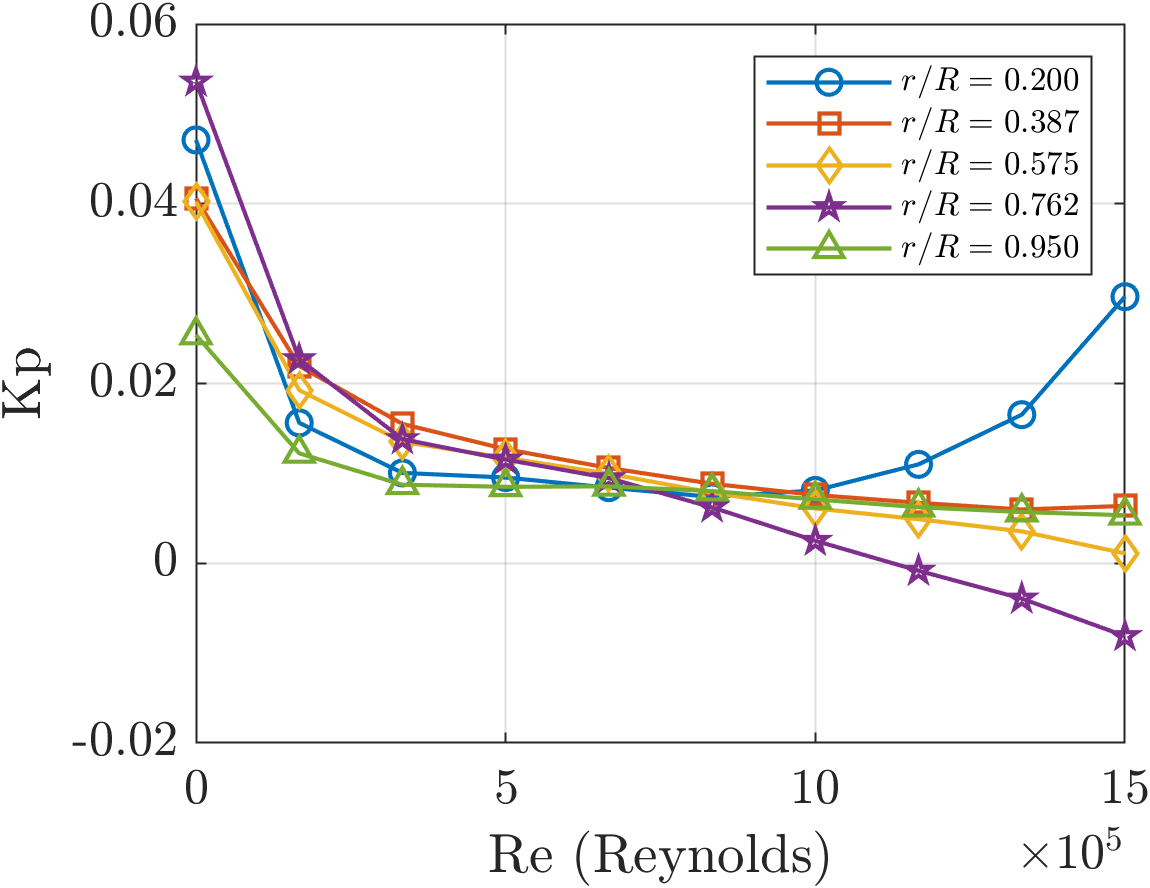
\includegraphics[width=0.39\textwidth]{Kp_2D.png}
        \caption{Relationship between $K_p$ and $Re$ along the blade}
        \label{fig:kp}    
\end{figure}

% \begin{figure}[H]
% \centering

%     \begin{minipage}{0.39\textwidth}
%         \centering
%         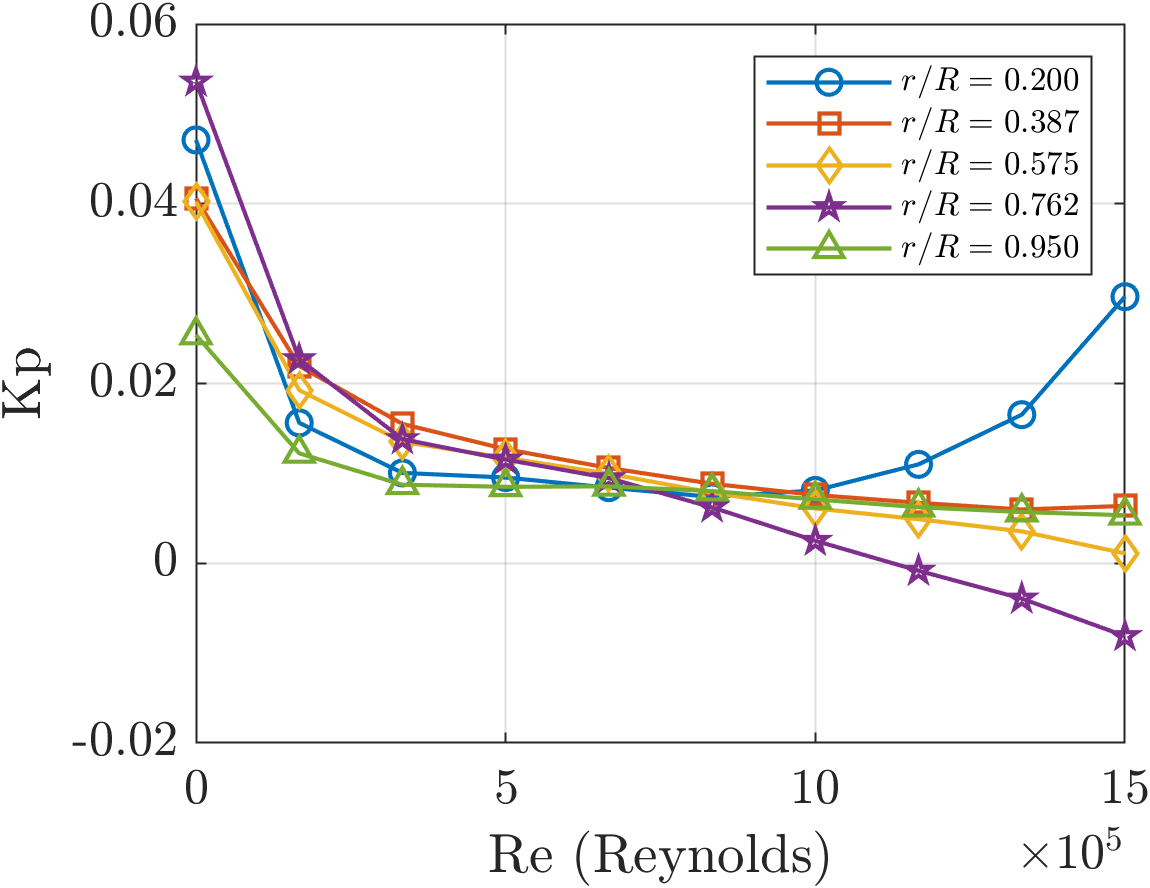
\includegraphics[width=\textwidth]{Kp_2D.png}
%         \caption{Relationship between $K_p$ and $Re$ along the blade}
%         \label{fig:kp}
%     \end{minipage}
%     \hfill
%     \begin{minipage}{0.39\textwidth}
%         \centering
%         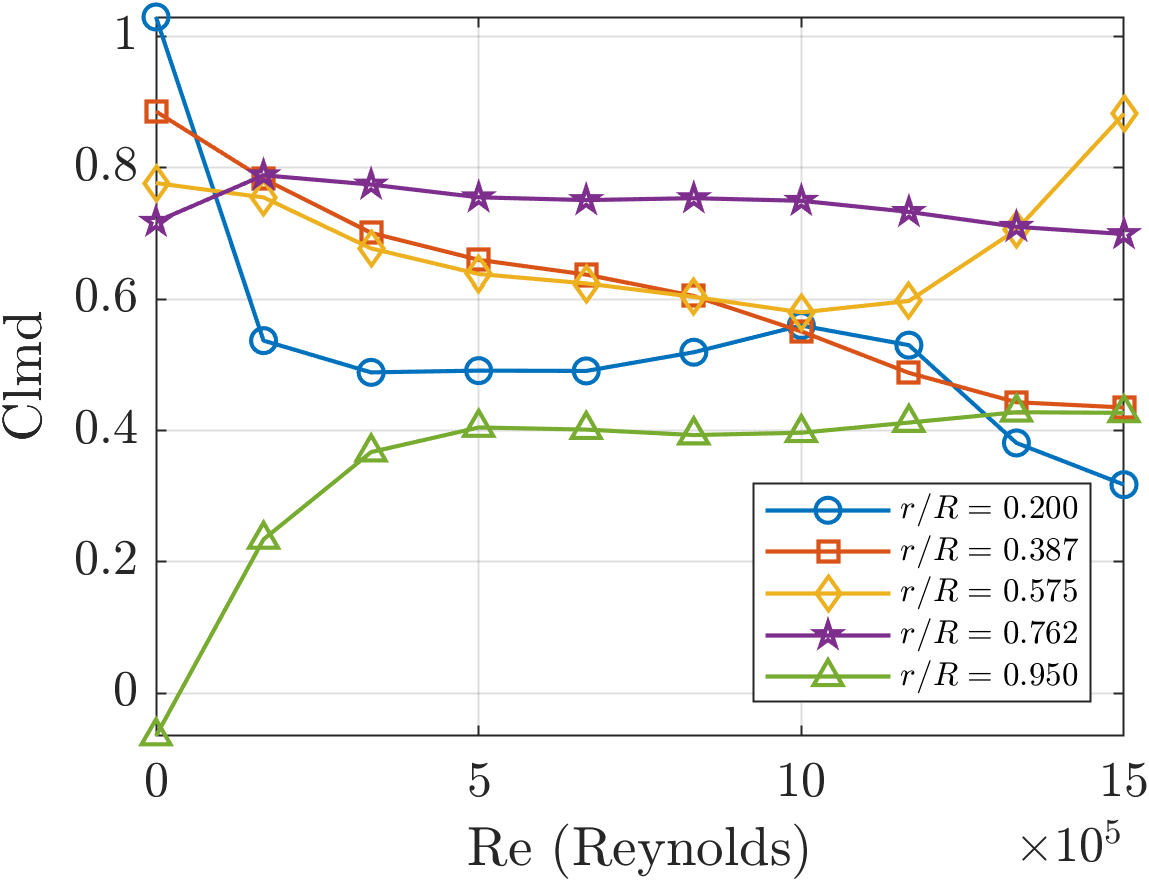
\includegraphics[width=\textwidth]{Clmd_2D.png}
%         \caption{Relationship between $C_{lmd}$ and $Re$ along the blade}
%         \label{fig:Clmd}
%     \end{minipage}
%     \hfill
%     \begin{minipage}{0.39\textwidth}
%         \centering
%         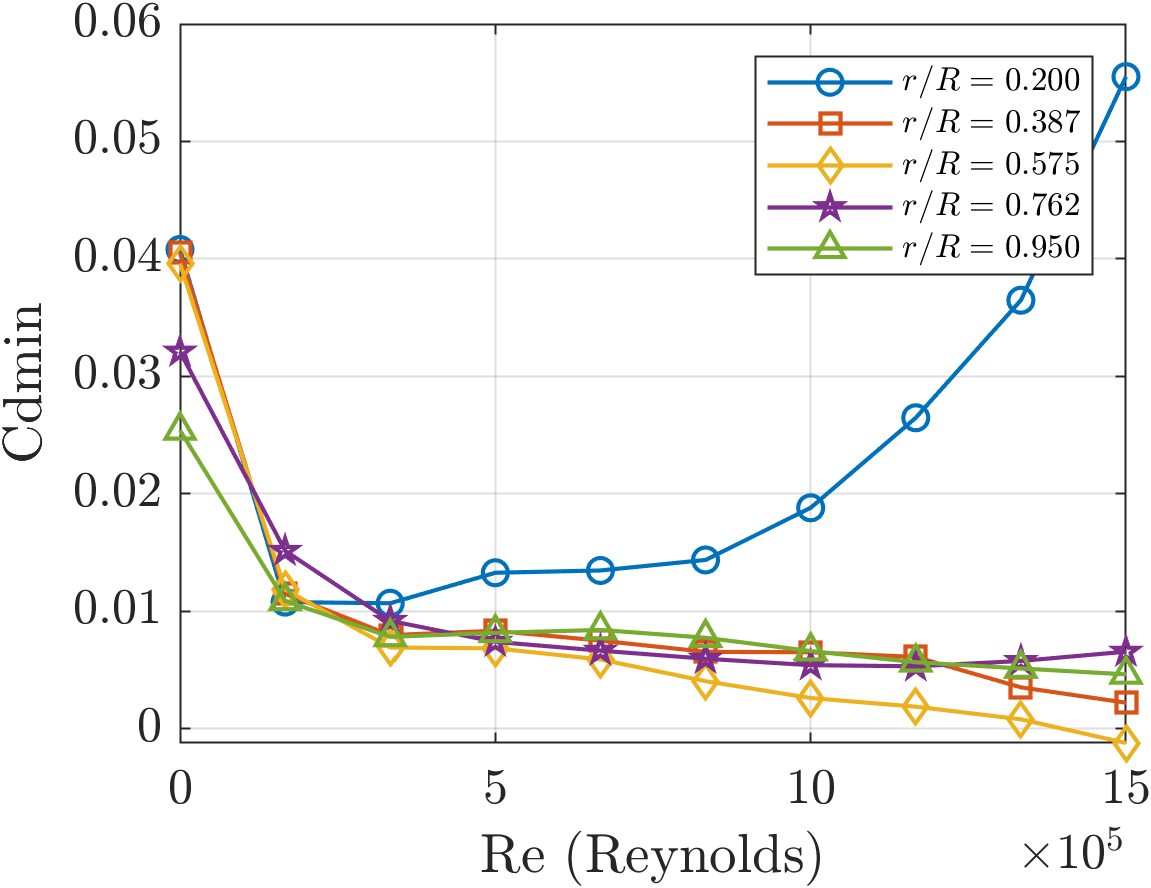
\includegraphics[width=\textwidth]{Cdmin_2D.png}
%     \caption{Relationship between $C_{dmin}$ and $Re$ along the blade}
%     \label{fig:Cdmin}
% \end{minipage}
% \end{figure}



\begin{table}[h!]
    \centering
    \begin{minipage}{0.45\textwidth}
        %\adjustbox{valign=m}{
            \centering % Center the content of Algorithm 4
            \begin{algorithm}[H]
                \caption{Coefficient Calculation with X-FOIL}\label{alg:xfoil_coeff_calculation}
                \begin{algorithmic}[1]
                    \State \textbf{Inputs:} 
                    \begin{itemize}
                        \item Range of Reynolds numbers: $[5000, 2000000]$ (increments of $5000$)
                        \item Range of angles of attack: $[-5^\circ, 15^\circ]$ (increments of $1^\circ$)
                        \item Geometry of each blade section (five sections)
                    \end{itemize}
                    \State Create an empty table to store results: $resultsTable$
                    \For{each Reynolds number $Re \in [5000, 2000000]$}
                        \For{each angle of attack $\alpha_{attack} \in [-5^\circ, 15^\circ]$}
                            \State Prepare input file for X-FOIL with the following parameters:
                            \begin{itemize}
                                \item Load airfoil geometry for each blade section
                                \item Set Reynolds number $Re$
                                \item Set angle of attack $\alpha_{attack}$
                                \item Define panel parameters (e.g., number of panels)
                            \end{itemize}
                            \State Run X-FOIL with the prepared input file
                            \State Obtain lift and drag coefficients ($C_L$, $C_D$) from X-FOIL outputs
                        \EndFor
                        \State Calculate variables $c_{lmd}$, $c_{d_{min}}$, and $k_p$ based on $C_L$ and $C_D$
                        \State Store results in the table with columns: $Re$, $c_{lmd}$, $c_{d_{min}}$, $\alpha_{stall}$, $c_{l_{\alpha}}$, $k_p$
                        \State Compute average $\alpha_{stall}$ and $c_{l_{\alpha}}$
                        \State Plot $c_{lmd}$, $c_{d_{min}}$, and $k_p$ vs Reynolds number
                    \EndFor
                    \State Save the results table to an \textbf{Excel file (.xlsx)} for further analysis
                \end{algorithmic}
            \end{algorithm}
        %} % End of adjustbox
    \end{minipage}
    \hfill
    \begin{minipage}{0.45\textwidth}
        %\adjustbox{valign=m}{
            \centering % Center the content of Algorithm 5
            \begin{algorithm}[H]
                \caption{Torque ($Q$) and Thrust ($T$) Calculation using the Traub Model}\label{alg:torque_thrust_calculation}
                \begin{algorithmic}[1]
                    \State \textbf{Inputs:} number of blades, initial/final angle, density, viscosity, divisions, angular velocity
                    \State \textbf{Regression:} Perform polynomial regression on blade section variables, including $c_{l_{\alpha}}$, $\alpha_{\text{stall}}$, $\alpha_{\text{zl}}$, $k_{\text{p}}$, $c_{d_{min}}$, and $c_{l_{md}}$.
                    \State Adjust regressions for each blade section and divide according to the number of propeller divisions.
                    \For{each blade section $i$ from $1$ to the number of divisions}
                        \State Compute $F_{\text{loss}}(i)$, $\alpha_{\text{inf}}(i)$, $\alpha_{\text{ind}}(i)$, $\alpha_{\text{attack}}(i)$, $X$, and $Re(i)$.
                        \State \textbf{Coefficient Correction:}
                        \State Interpolate $c_{d_{min}}$, $k_p$, and $c_{l_{md}}$ using $Re(i)$.
                        \State Compute $c_{d_{\text{corrected}}}(i)$ and $c_{l_{\text{corrected}}}$.
                        \State \textbf{Integrands for Torque and Thrust:}
                        \State Compute integrands $integrand1(i)$ and $integrand2(i)$ using corrected $c_d$ and $c_l$, $\alpha_{\text{inf}}$, $\alpha_{\text{ind}}$, and chord $c$.
                    \EndFor
                    \State \textbf{Torque and Thrust:} Integrate $integrand1$ and $integrand2$ to obtain the total $Q$ and $T$.
                \end{algorithmic} 
            \end{algorithm}
        %} % End of adjustbox
    \end{minipage}
\end{table}


To obtain propeller thrust and torque, calculations were performed supporting in XFOIL software, as mentioned in \cite{Castellanos2023Propeller}, to determine the parameters influencing the lift and drag coefficients, which are involved in these two variables. This approach allowed for a detailed examination of how these coefficients vary under changing conditions, incorporating stall and boundary layer separation effects, which enhance the understanding of torque and thrust calculations using TRAUBS theory. Additionally, it accounts for tip losses and boundary layer compressibility, as well as the stall angle, previously mentioned, to represent the full propeller phenomena.


To implement Traub's theory through XFOIL, it was necessary to obtain key aerodynamic parameters: $K_{p}, C_{lmd}, C_{dmin},$ $C_{l\alpha}$ and $\alpha_{stall}$ as defined by \autoref{fig:Traub} and explained in \autoref{fig:aero_coefficients}. The process began by discretizing the McCauley propeller blade and conducting a 3D scan to gather the transverse coordinates along its profile. Five representative cross-sectional areas were then selected, and the coordinates were normalized (review procedure on \cite{Castellanos2023Propeller}), as XFOIL requires input coordinates in a normalized format rather than absolute values.


Following this, a MATLAB algorithm \ref{alg:xfoil_coeff_calculation} was used to automate the execution of XFOIL for each of the five selected sections. This code varied the angle of attack over a specified range of Reynolds numbers obtaining from XFOIL $C_{L}$ and $C_{D}$ coefficients for each atack angle, and following equations produced a CSV file for each blade section that included the extracted Traub parameters. These CSV files were subsequently processed in Excel, where polynomial regression was applied to characterize the behavior of these parameters as functions of the Reynolds number.
\par % Asegura el fin del párrafo anterior
\vspace{15pt}
\begin{mdframed}[
    innermargin=3pt,
    innertopmargin=0pt,
    innerbottommargin=3pt,
    linewidth=1pt,
    roundcorner=5pt
]
    \begin{multicols}{2}
        \begin{itemize}[leftmargin=*, noitemsep, topsep=0pt, parsep=0pt, partopsep=0pt]
            \item $C_{\text{lmd}} = C_{L}$ at the Angle of Attack $\alpha$ where $C_{D}$ is minimum
            \item $C_{\text{dmin}} = C_{D}$ at its minimum value
            \item \mbox{$C_{l\alpha} =$ Slope of the $C_{L}$ vs. Angle of Attack $\alpha$ curve}
            \item $\alpha_{\text{stall}} =$ Angle of Attack $\alpha$ where $C_{L}$ is maximum
            \item $K_{p} =$ Slope of the $C_{D}$ vs. $(C_{L} - C_{\text{lmd}} )^2$ curve
        \end{itemize}
    \end{multicols}
\end{mdframed}

\captionsetup{type=figure, skip=0pt}
\captionof{figure}{List of Aerodynamic Coefficients of XFOIL - \textit{Description}}
\label{fig:aero_coefficients}

\vspace{15pt}

The polynomial coefficients obtained from the regressions were then imported into MATLAB and, specifically, Simulink, where a multi-polynomial regression was performed to interpolate the Traub parameters for the selected cross-sectional areas of the blade. Ten blade sections were chosen as they significantly improved the aerodynamic description of the blade; beyond this number, the additional accuracy became minimal, while the computational cost increased substantially, causing the Simulink simulation time to grow significantly.

\vspace{10pt}
\subsection{PID controller - Governor Implementation}

Regarding the PID control, the procedure outlined in Chapter 1 was implemented and integrated directly into the Simulink model. Several iterations were conducted to determine the optimal \( K \) coefficients (Proportional, Integral and Derivative), aiming to ensure that the variables conditioning the engine (Torque, Pitch Angle, and propeller RPM) operate within the established ranges outlined in \autoref{tab:torque_conditions}, were pitch angle varies from 22° to 84.5° and torque from 1000 Nm to 3000 Nm; and as specified in \cite{Piper1998}, RPM should be below 2200. The simulation obtained from the PID control, appears in \autoref{fig:Turboprop_Pitch_Angle_1}. It shows the way PID varies pitch angle according differents torque requirements during flight stages, contrasting information in \autoref{tab:torque_conditions}, the pitch angle variation is similar to operation conditions.

\begin{figure}[H]
    \centering
    {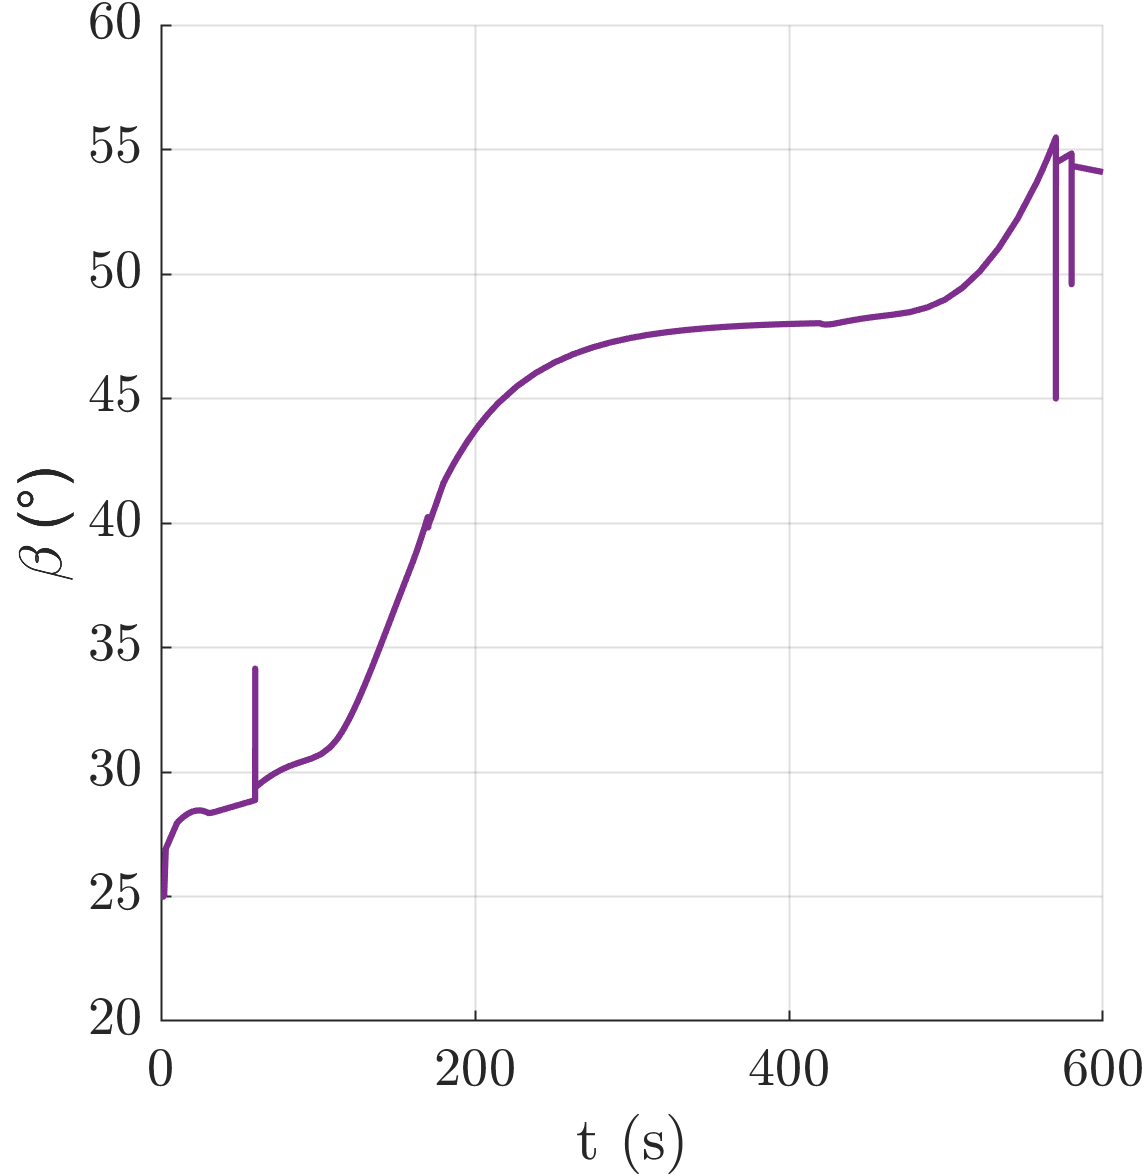
\includegraphics[width=0.3\textwidth]{n_beta - copia.png}}
    \caption{PID Control on Pitch Angle}
    \label{fig:Turboprop_Pitch_Angle_1}
\end{figure}

To guide the PID controller, a set of nominal torque values was defined for each phase of flight, providing target values for the controller to track. The nominal torque function, implemented in MATLAB, specifies desired torque levels across different time intervals corresponding to various stages of flight, such as taxing, takeoff, cruise, approach, and deceleration after landing. This approach ensures that the PID controller continuously adjusts the system to meet the torque requirements of each specific phase.


The nominal torque parametrization is explained in Algorithm \autoref{alg:torque_calculation}. After iterating with various values for the entire system, the PID coefficients that yielded the most accurate response compared to operational design specification (Torque, Pitch Angle, and propeller RPM), were found to be \( K_p=0.001 \), \( K_i=0.0001 \), and \( K_d=0.0001 \). This combination of coefficients enabled the controller to maintain stable and responsive adjustments, ensuring that the system variables remained within their designated operational ranges throughout all flight stages.


%%The nominal torque parametrization is explained in Algorithm \autoref{alg:torque_calculation}.After iterating with various values the whole system, the PID coefficients that yielded the most effective response were found to be \( K_p=0.001 \), \( K_i=0.0001 \), and \( K_d=0.0001 \). This combination of coefficients enabled the controller to provide stable and responsive adjustments to meet the torque requirements across all flight stages.



\begin{algorithm}
\caption{Nominal Torque Calculation During Flight Stages}\label{alg:torque_calculation}
\begin{algorithmic}[1]

\State \textbf{Input:} $t$ (current time)

\State \textbf{Constants:} $\tau_{\text{idle-taxiing}}, \tau_{\text{takeoff}}, \tau_{\text{cruise}}, \tau_{\text{approach}}, \tau_{\text{landing}}, \tau_{\text{deceleration}}$ \Comment{Nominal torques for each flight stage}

\If{$t \leq t_{\text{taxiing end}}$}
    \State $\tau_{\text{nom}} \gets \tau_{\text{taxiing}}$ \Comment{Idle - Taxiing phase}
    
\ElsIf{$t_{\text{taxiing end}} < t \leq t_{\text{takeoff end}}$}
    \State $\tau_{\text{nom}} \gets \tau_{\text{takeoff}}$ \Comment{Takeoff phase}
    
\ElsIf{$t_{\text{takeoff end}} < t \leq t_{\text{cruise end}}$}
    \State $\tau_{\text{nom}} \gets \tau_{\text{cruise}}$ \Comment{Cruise phase}
    
\ElsIf{$t_{\text{cruise end}} < t \leq t_{\text{approach end}}$}
    \State $\tau_{\text{nom}} \gets \tau_{\text{approach}}$ \Comment{Approach phase}
    
\ElsIf{$t_{\text{approach end}} < t \leq t_{\text{landing end}}$}
    \State $\tau_{\text{nom}} \gets \tau_{\text{landing}}$ \Comment{Landing approach phase}
    
\Else
    \State $\tau_{\text{nom}} \gets \tau_{\text{deceleration}}$ \Comment{Deceleration after landing}
    
\EndIf
\State \textbf{Output:} $\tau_{\text{nom}}$ (nominal torque)
\end{algorithmic} 
\end{algorithm}



\section{Verification Section: \emph{To evaluate the accuracy of the quantitative predictions obtained with respect to experimental data or other computational techniques used in the industry, available in specialized literature.}}\label{sec:Method}

This section describes the process of validating the computational model, which is divided into three main sections: the engine, the propeller, and the integrated engine-propeller system. In the engine validation, parameters such as pressure ratio, temperature, and revolutions of the gas generation shaft are analyzed to ensure the engine operates within expected parameters that appears in \cite{Castellanos2019} and \cite{Piper1998}. Then, the propeller is validated by evaluating torque, thrust, RPM, and the pitch angle to ensure its behavior aligns with operational standards stablish in \cite{Castellanos2023Propeller} and \cite{Piper1998}. Finally, the complete system, which includes governor control, is validated to guarantee the stability and overall performance through efficiencies (thermal and propulsion)  of the architecture during flight phases such as takeoff, cruise, and descent, ensuring that the model accurately represents real-world conditions mentioned in \cite{Castellanos2023Propeller}, \cite{Piper1998}, \cite{book:96630002}, \cite{stengel2024power} and \cite{pulido2008conversión}.

In order to validate the proposed architecture, a small aircraft on a short route was chosen to simulate the flight conditions, using a path from El Dorado Airport to Guaymaral Airfield as a reference. This route, estimated at 600 seconds, let structure the simulation into several phases representative of a real flight. It was defined a 60 seconds engine startup, 120 seconds as takeoff, 240 seconds for cruise, and 180 seconds descent and landing. Based on this estimated time, key variables such as fuel mass flow, altitude, pressure, temperature, density, and dynamic viscosity were adjusted according to these flight phases, in order to more accurately replicate the real operating conditions and ensure proper system validation.

The fuel mass flow varies linearly from 0 kg/s to 0.03 kg/s, stabilizes, then increases to 0.06 kg/s, and finally decreases linearly to 0.01 kg/s following requirements stablish in \cite{Piper1998} . The parameters of density, pressure, temperature, and dynamic viscosity change as functions of altitude, following equations \ref{eq:temp}, \ref{eq:pressure}, \ref{eq:density}, \ref{eq:viscosity}. Altitude begins at 0 m, increases linearly to 3800 m, remains stable, and then decreases back to 0 m. Airspeed starts at 2 m/s, increases linearly to 50 m/s, stabilizes, and then returns to 2 m/s.

In contrast, for the simulation of the engine and propeller alone, only the fuel mass flow variation was taken into account, while the other parameters (altitude, pressure, temperature, density, viscosity) were kept constant, as if conducting a ground test. This approach was used to isolate and analyze the engine-propeller behavior under controlled conditions, allowed to simulate flight conditions by changing these variables in the third validation, where the integrated engine-propeller system was assessed with full dynamic control.

\subsection{Engine Validation}

\autoref{fig:Compression_Stage_Results} and  \autoref{fig:Turbine_Stage_Results} display simulation results for the compressor and turbine stages of a turboprop engine, showing the transient behavior of pressure and temperature over time. These stages are transient due to progressive fuel injection, allowing gradual stabilization of operating conditions. In the compression stage, pressure and temperature increase through the three axial compressors and the centrifugal compressor, with the latter contributing most significantly. In the turbine stage, pressure decreases and temperature stabilizes as energy is extracted from the gases. For this model validation, standard atmospheric conditions were set at 1 atm (101.33 kPa) and 288 K (15°C), simulating ground-level operation. To replicate the propeller effect during stationary testing, a constant torque load of 2600 N.m was applied to the turbines, rather than connecting them directly to the propeller. The fuel mass progressively reached a maximum of 0.06 kg/s, while the gas generation shaft RPM was initialized at 12000, and it increased significantly under normal operating conditions, reaching up to 41980.60 RPM at cruise, establishing a baseline for engine performance.

\begin{figure}[h]
    \centering
    \begin{subfigure}[b]{0.47\textwidth}
        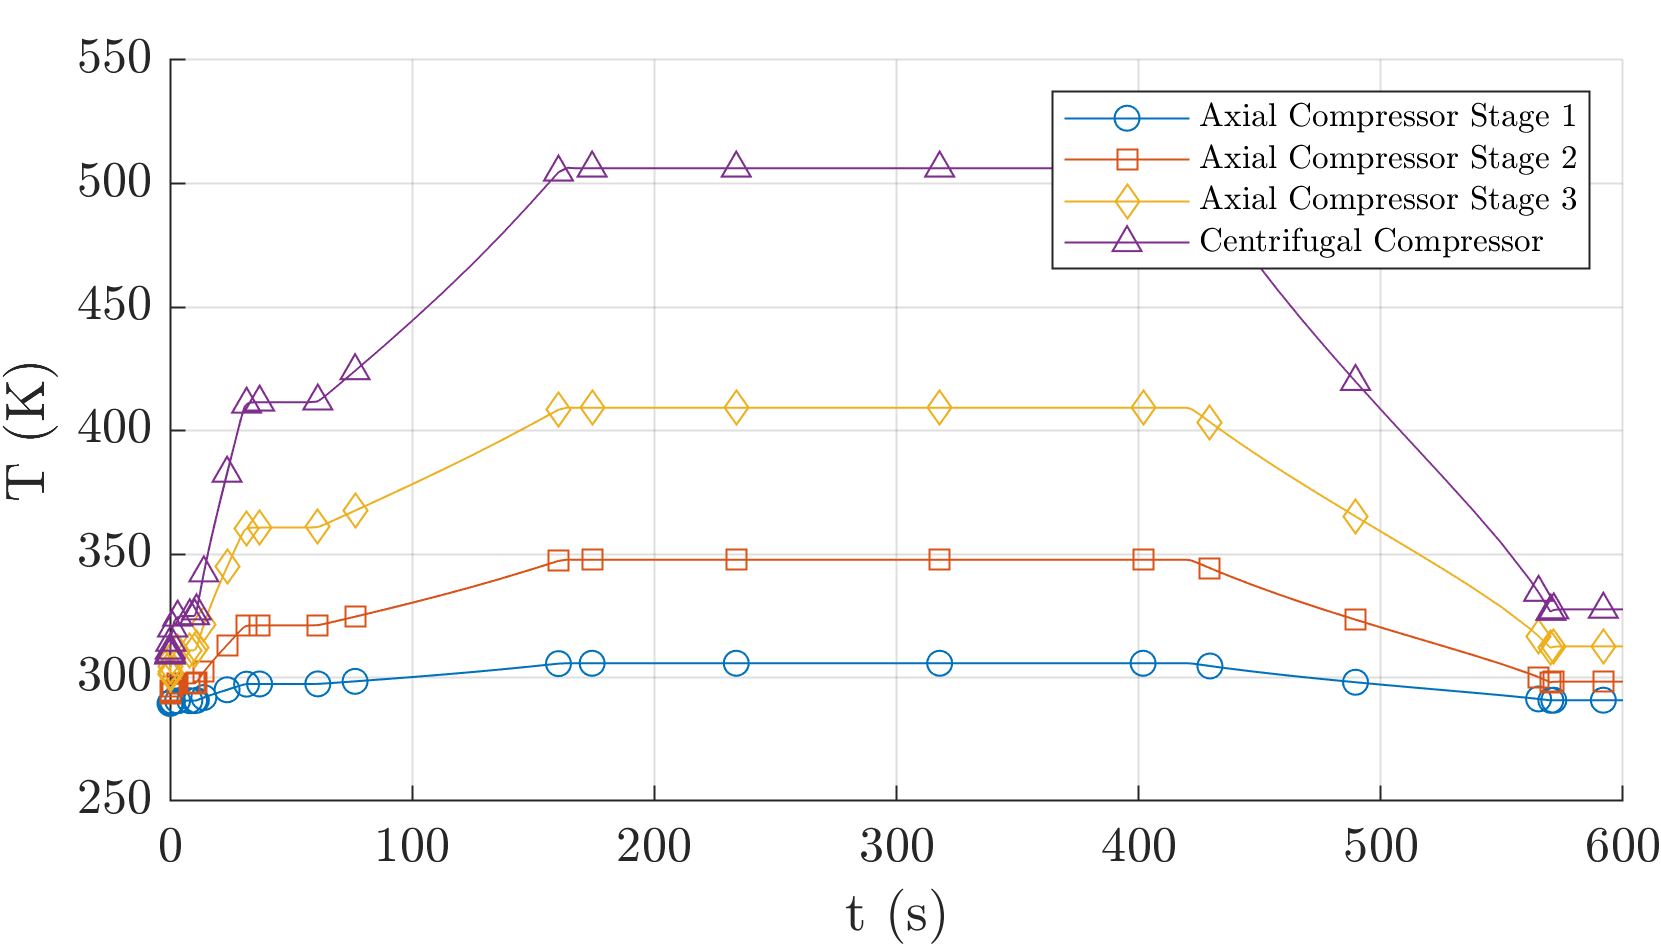
\includegraphics[width=\textwidth]{T_compresion.png}
        \caption{Graph 1: Compression Stage -  Temperature}
        \label{fig:T_compresion}
    \end{subfigure}
    \hspace{0.02\textwidth}
    \begin{subfigure}[b]{0.47\textwidth}
        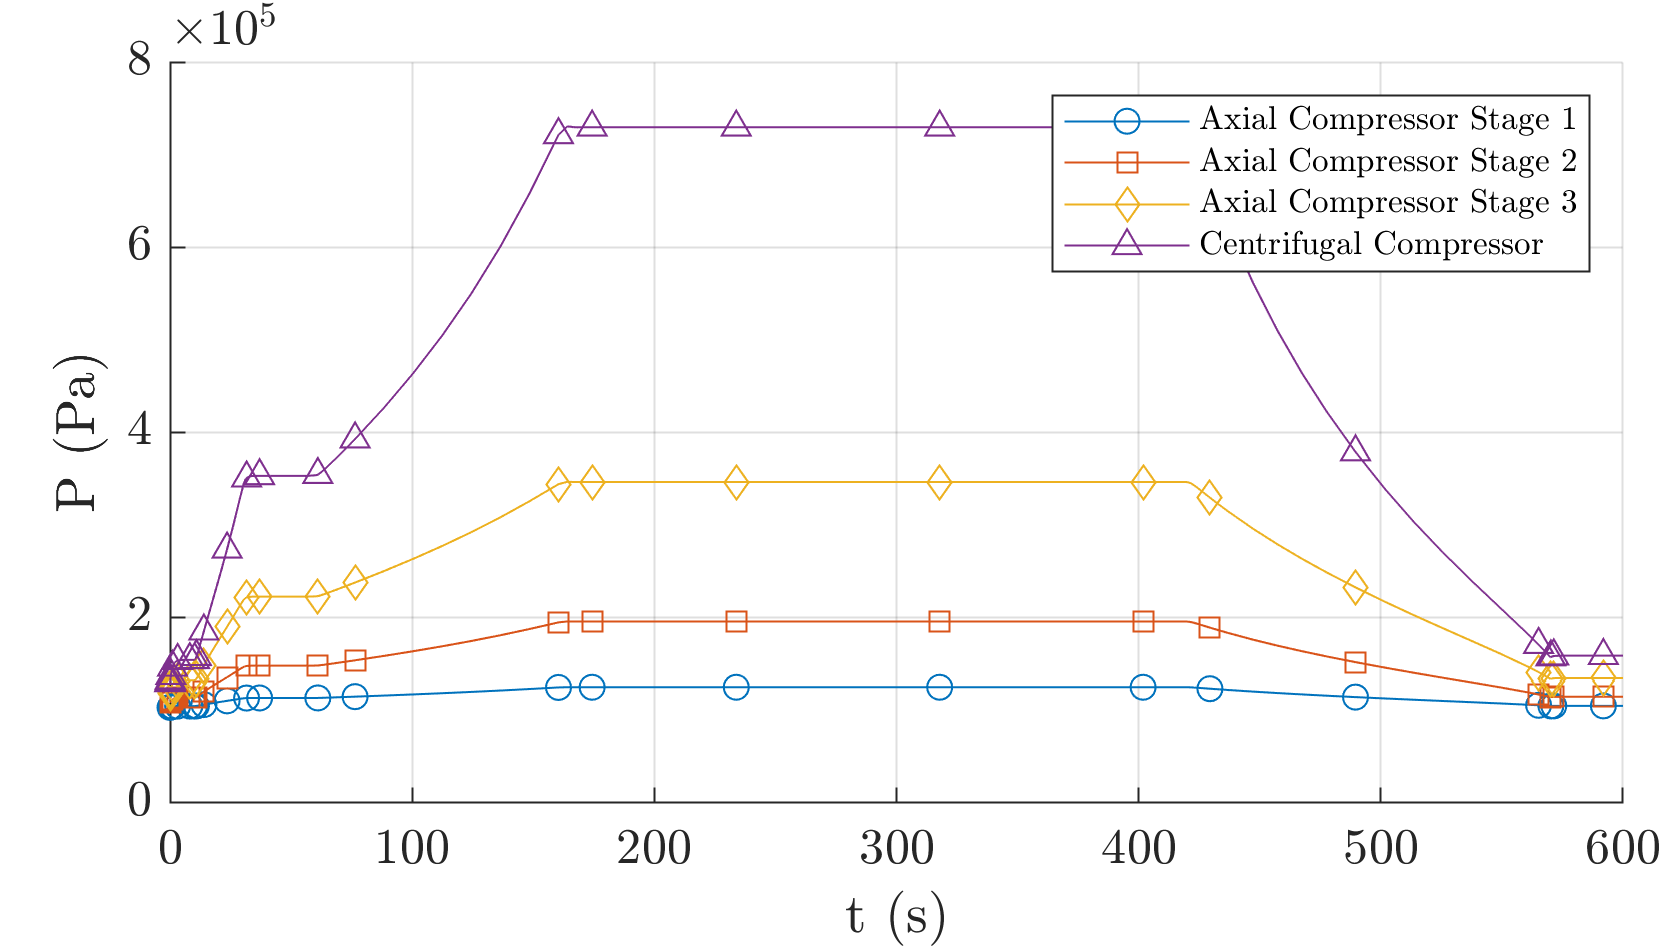
\includegraphics[width=\textwidth]{P_compresion.png}
        \caption{Graph 2: Compression Stage -  Pressure}
        \label{fig:P_compresion}
    \end{subfigure}
    \vskip\baselineskip
    \caption{Compression Stage Results}
    \label{fig:Compression_Stage_Results}
\end{figure}
\vspace{0.375cm}

\begin{figure}[h]
    \centering
    \begin{subfigure}[b]{0.47\textwidth}
        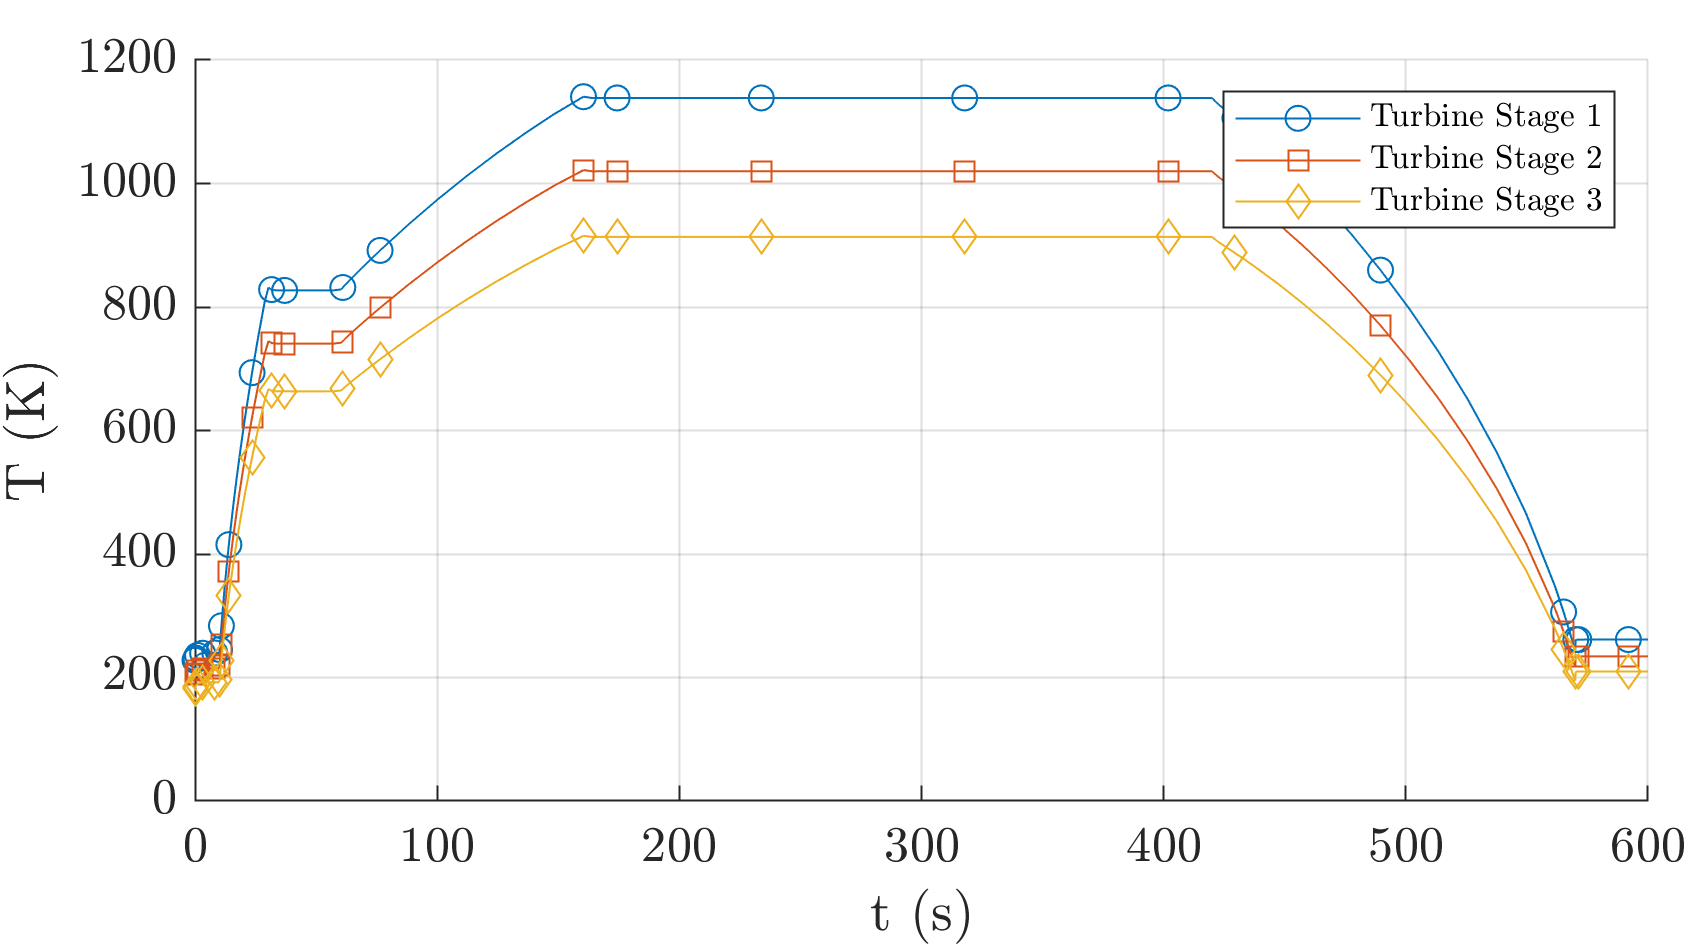
\includegraphics[width=\textwidth]{T_turbina.png}
        \caption{Graph 1: Turbine Stage -  Temperature}
        \label{fig:T_compresion}
    \end{subfigure}
    \hspace{0.02\textwidth}
    \begin{subfigure}[b]{0.47\textwidth}
        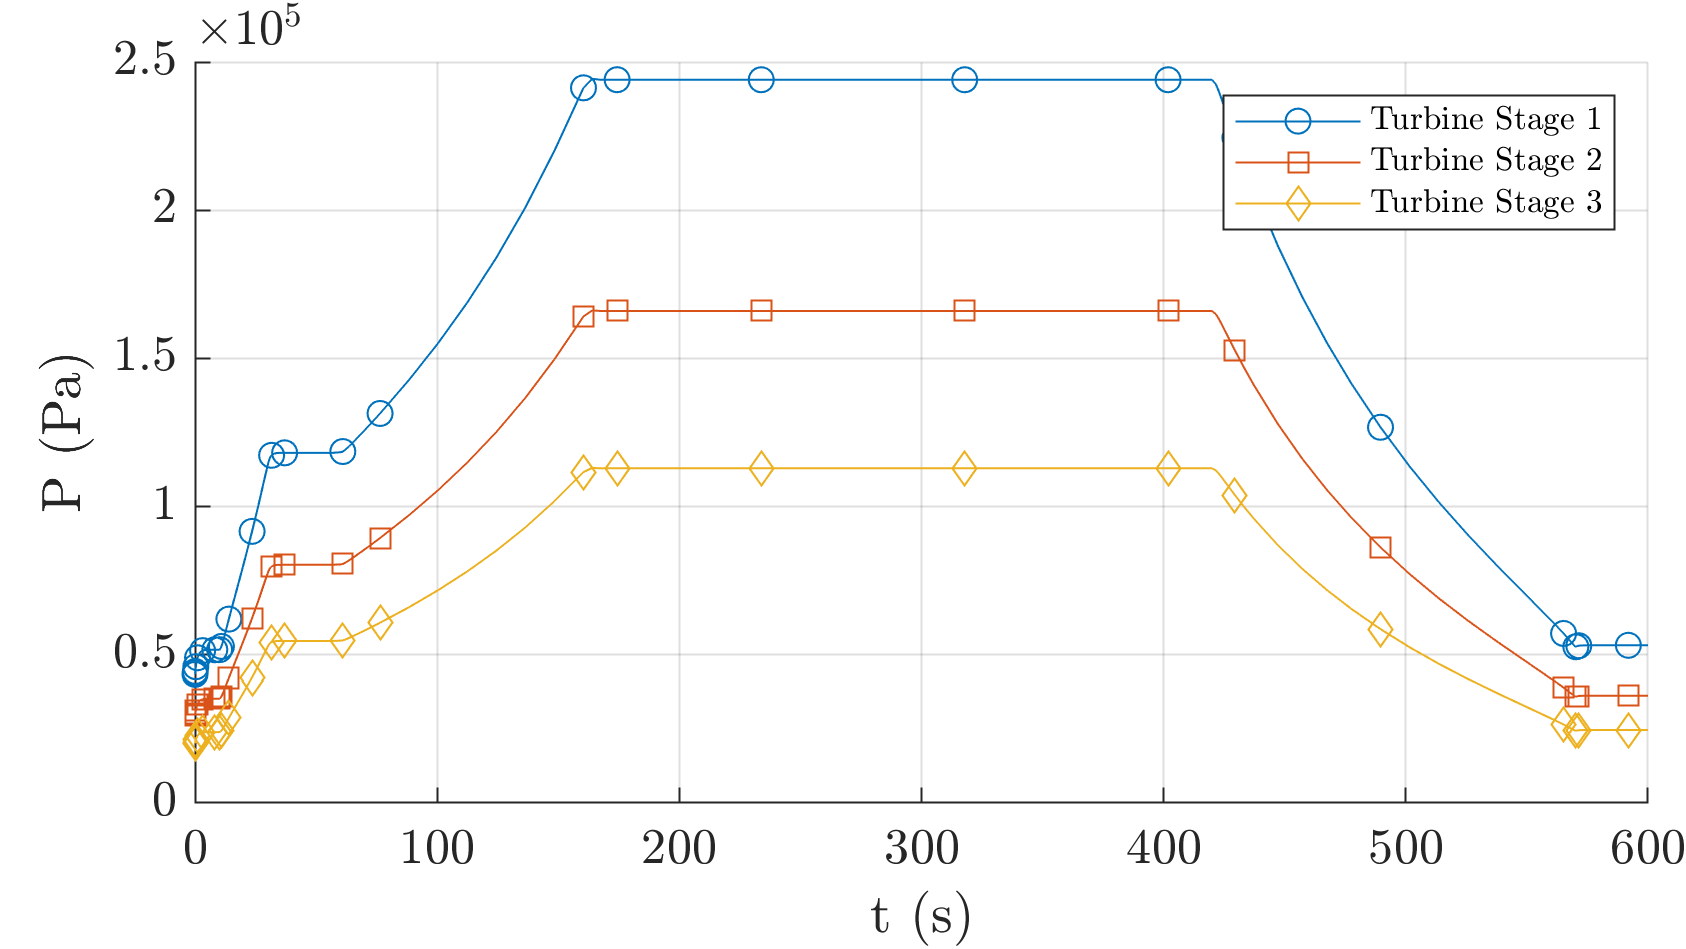
\includegraphics[width=\textwidth]{P_turbina.png}
        \caption{Graph 2: Turbine Stage -  Pressure}
        \label{fig:P_compresion}
    \end{subfigure}
    \vskip\baselineskip
    \caption{Turbine Stage Results}
    \label{fig:Turbine_Stage_Results}
\end{figure}
\vspace{0.375cm}

With these parameters firmly established, the simulation was conducted to obtain critical performance outputs: pressure within the centrifugal compressor, temperature at the inlet of the gas generation turbine, and RPM values of the gas generation shaft. These results were then meticulously cross-referenced with standard values specified in the engine manual \cite{Castellanos2019,Piper1998} to confirm the model’s alignment with expected real-world operational benchmarks.


The comparison between the simulation results and the reference data from the PT6 engine manual is presented in \autoref{table:model_reference_comparison}. The close agreement between the model values and the reference values—demonstrated by the low percentage errors in compressor pressure, combustion temperature, and gas generation shaft speed—validates the accuracy of the simulation under ground-level conditions. These parameters were specifically analyzed, as they are critical and, if not modeled correctly, could lead to anomalies in performance or even structural failures in the actual engine. This comparison ultimately corroborates that the model effectively replicates the engine's behavior within an acceptable margin of error, supporting its reliability for further analyses.

\begin{table}[h!]
    \centering
    \begin{tabular}{|l|c|c|c|c|}
        \hline
        \textbf{Engine Parameter} & \textbf{Symbol} & \textbf{Model Value} & \textbf{Reference (PT6 Manual)} & \textbf{Error (\%)} \\
        \hline
        Compressor Pressure [kPa] & \( P_{cc} \) & 734.38 & 787.38 & 6.73 \\
        Combustion Temperature [K] & \( T_{t1} \) & 1225.00 & 1212.25 & 1.05 \\
        Gas Generation Shaft Speed [RPM] & \( N_g \) & 41980.60 & 40000.00 & 4.95 \\
        \hline
    \end{tabular}
    \vspace{10pt}
    \caption{Comparison of model results with PT6 manual reference data}
    \label{table:model_reference_comparison}
\end{table}





\subsection{Propeller Validation}

The results for propeller RPM, pitch angle, torque, and thrust are shown in \autoref{fig:Propeller_RPM_PitchAngle} and  \autoref{fig:TORQUE_THRUST_PROPELLER_VALIDATION} highlighting their dynamic responses across different flight stages: acceleration, cruise, and descent. The validation of the propeller used a setup combining the Traub model with the power generation shaft. A custom pitch angle schedule was directly applied to the Traub model, adjusting with each phase to meet the requirements outlined in \autoref{tab:torque_conditions} for optimal aerodynamic performance. The power values obtained from engine validation were input separately into the Simulink model of the propeller.


\begin{figure}[h]
    \centering
    \begin{subfigure}[b]{0.47\textwidth}
        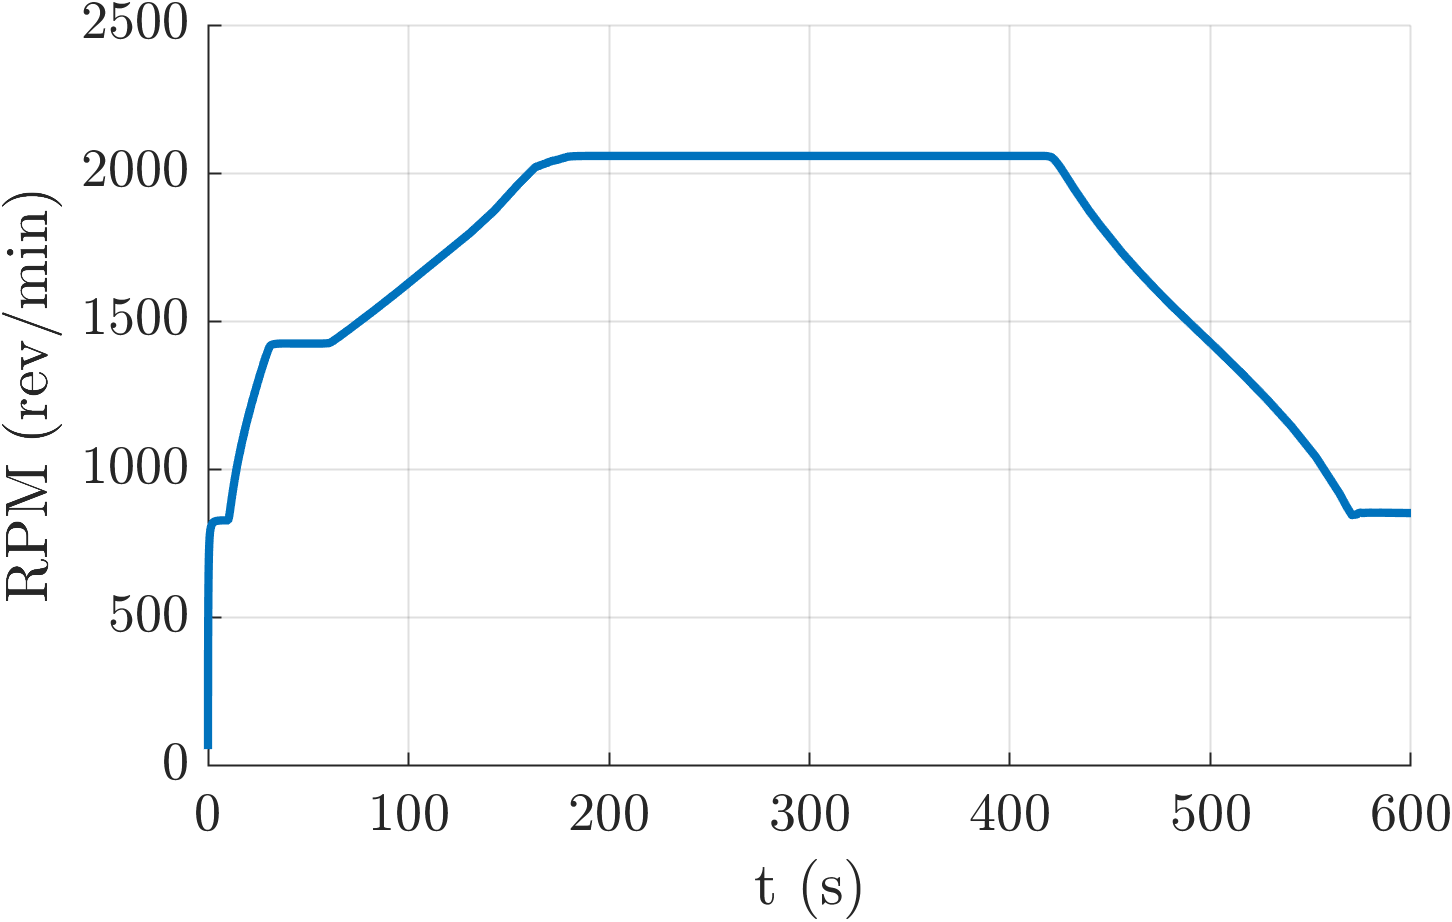
\includegraphics[width=\textwidth]{RPM_PROPELLER_VALIDATION.png}
        \caption{Propeller RPM Results}
        \label{fig:Propeller_RPM}
        \end{subfigure}
        \hspace{0.02\textwidth}
    \begin{subfigure}[b]{0.47\textwidth}
        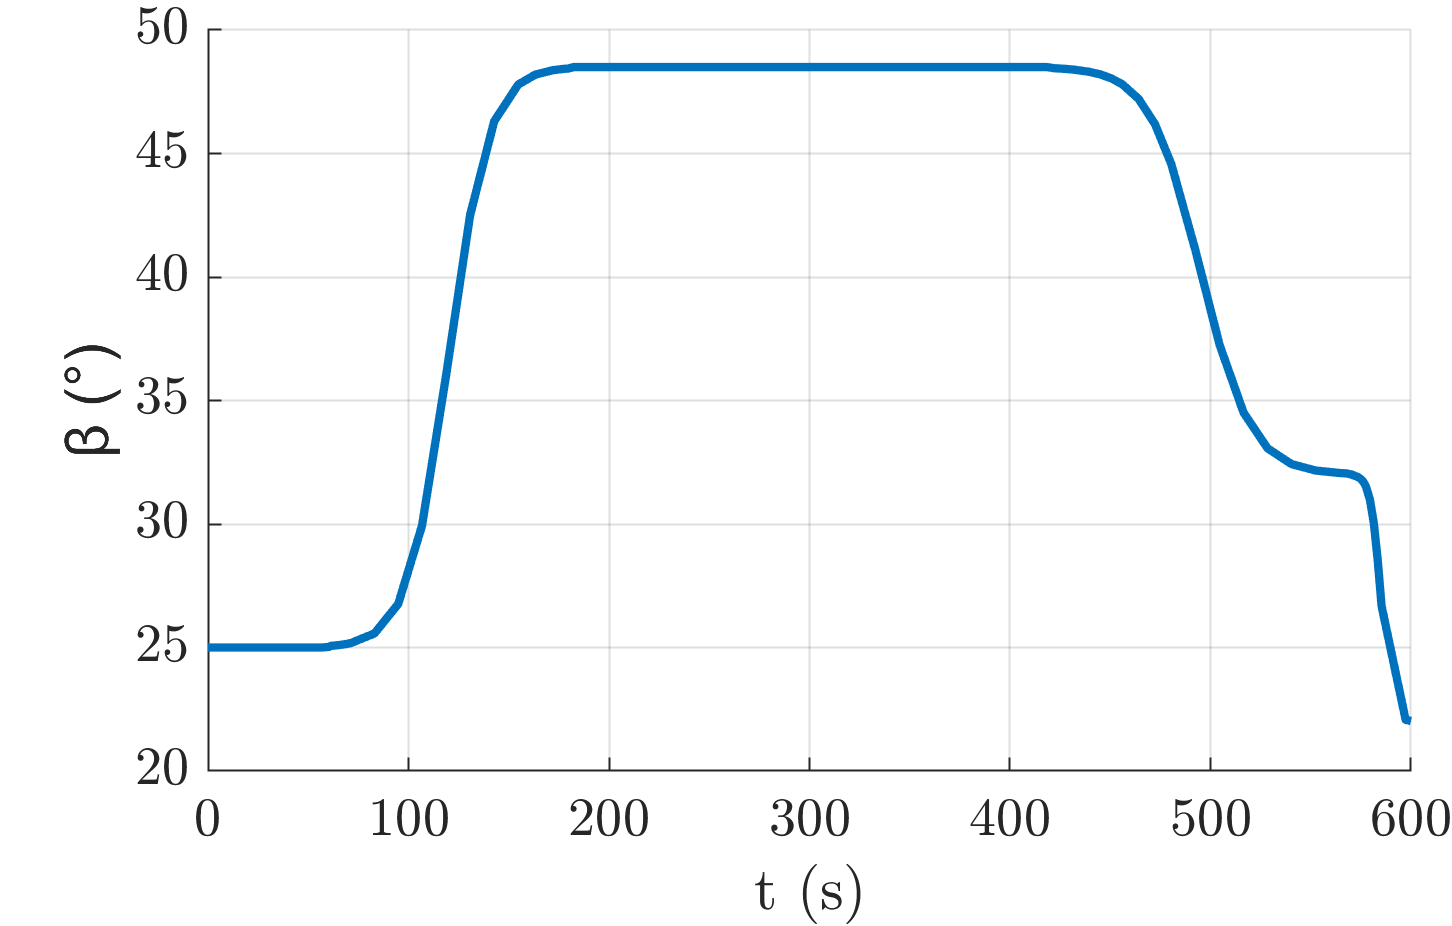
\includegraphics[width=\textwidth]{PITCH_PROPELLER_VALIDATION.png}
        \caption{Propeller Pitch Angle Results}
        \label{fig:Propeller_PitchAngle}
    \end{subfigure}
    %\vskip\baselineskip
    \vspace{15pt}
    \caption{Propeller RPM and Pitch Angle Results}
    \label{fig:Propeller_RPM_PitchAngle}
\end{figure}

\begin{figure}[h]
    \centering
    \begin{subfigure}[b]{0.47\textwidth}
        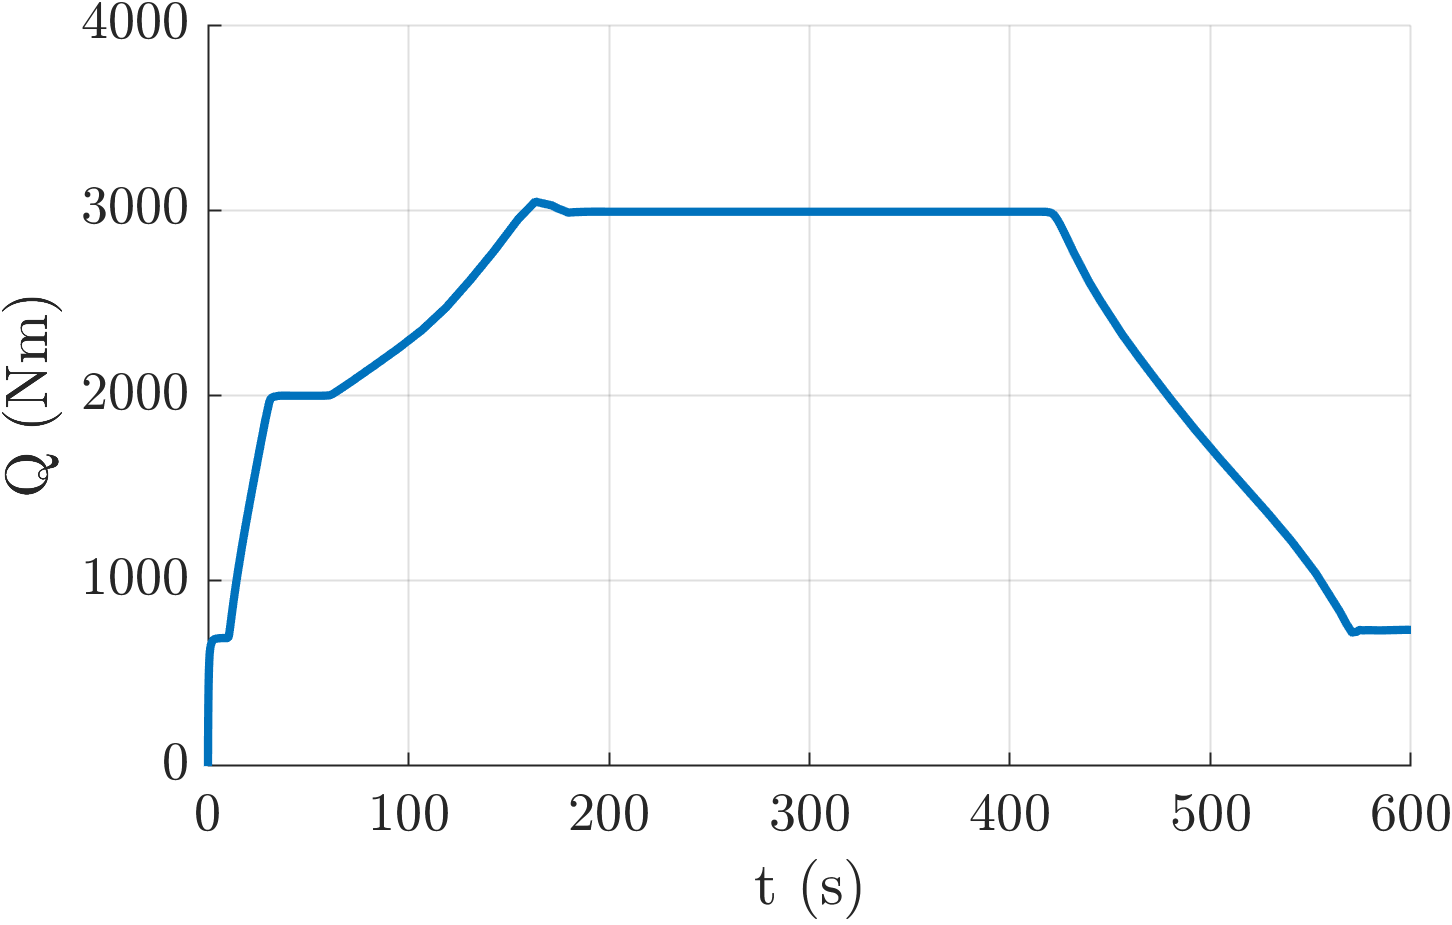
\includegraphics[width=\textwidth]{Q_PROPELLER_VALIDATION.png}
        \caption{Propeller Torque Results}
        \label{fig:TORQUE_PROPELLER_VALIDATION}
    \end{subfigure}
    \hspace{0.02\textwidth}
    \begin{subfigure}[b]{0.47\textwidth}
        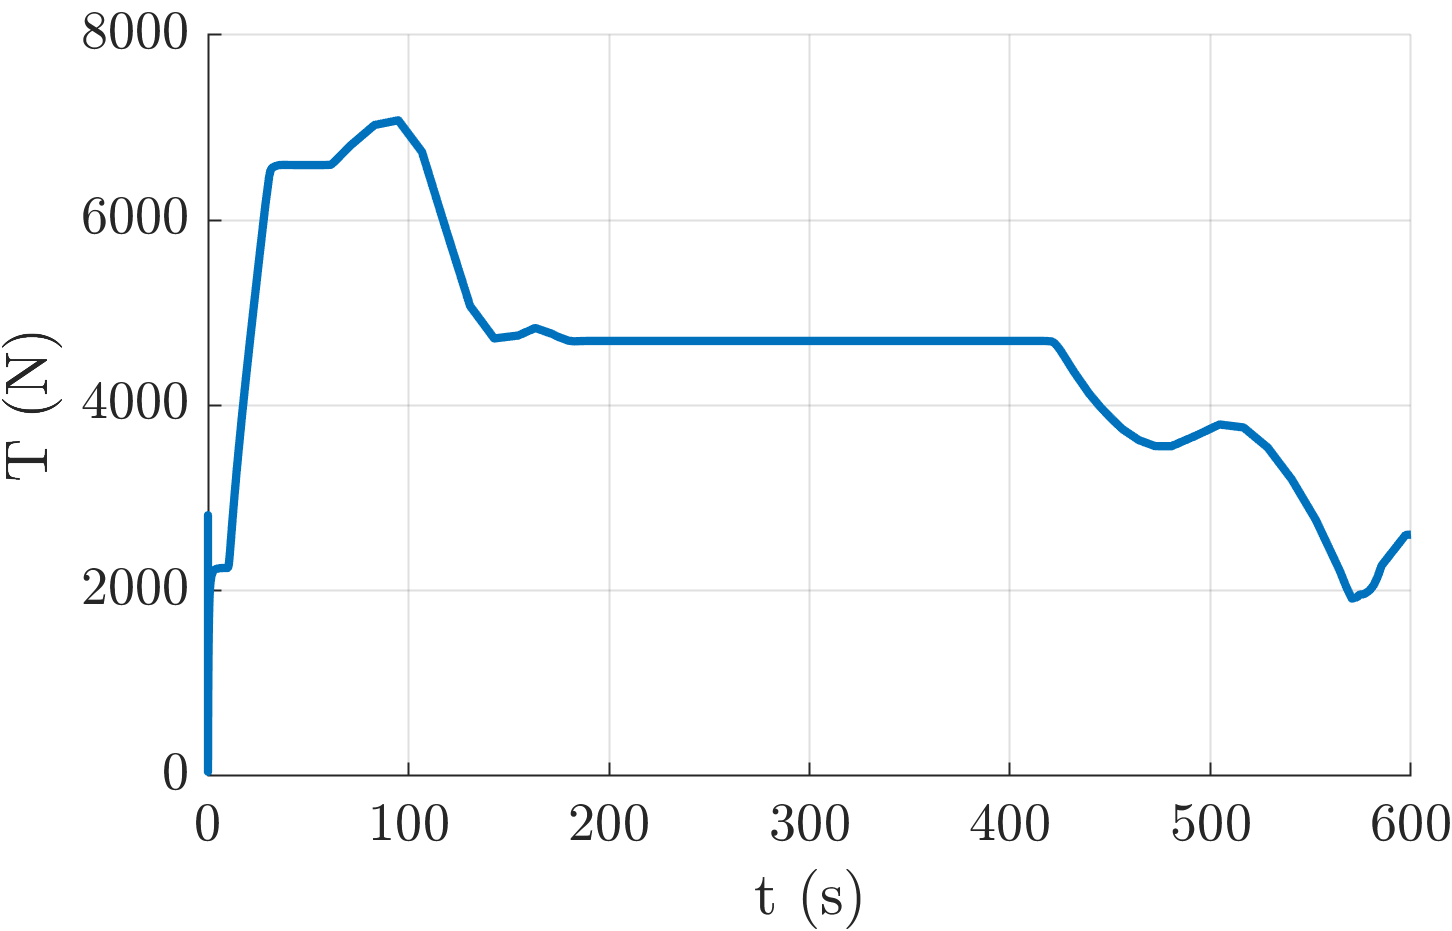
\includegraphics[width=\textwidth]{T_PROPELLER_VALIDATION.png}
        \caption{Propeller Thrust Results}
        \label{fig:THRUST_PROPELLER_VALIDATION}
    \end{subfigure}
    %\vskip\baselineskip
    \vspace{15pt}
    \caption{Propeller Torque and Thrust Results}
    \label{fig:TORQUE_THRUST_PROPELLER_VALIDATION}
\end{figure}



The obtained response of the propeller during simulation shows key performance aspects aligned with operational expectations. Firstly, the RPM remains consistently below the 2200 limit as shown in \autoref{fig:Propeller_RPM}, as stipulated in the engine manual, indicating effective control over rotational speed throughout the test. Additionally, the behavior of both torque and thrust correlates logically with variations in the pitch angle as in \autoref{tab:torque_conditions}. At lower pitch angles, thrust is maximized due to the increased aerodynamic efficiency, while torque remains lower. \autoref{fig:TORQUE_THRUST_PROPELLER_VALIDATION} shows that as the pitch angle increases as in \autoref{fig:Propeller_PitchAngle}, both torque and thrust initially rise. However, around the 80-second mark, thrust experiences a noticeable drop, attributable to the onset of stall. This aerodynamic stall prevents further thrust generation despite increases in pitch angle, marking a limit in the propeller’s performance under high-pitch conditions. Beyond this point, the system stabilizes, with the torque acting as a regulating factor that prevents the RPM from exceeding 2200, thus ensuring safe operation by balancing the propeller load effectively.

\begin{table}[h!]
    \centering
    \begin{tabular}{|l|c|c|}
        \hline
        \textbf{Conditions} & $\beta$ ($^\circ$) & \textbf{Torque (N$\cdot$m)} \\
        \hline
        Low-Speed Takeoff Roll & 22 & Far below max \\
        Takeoff speed & 32 & 3023 \\
        Maximum Low-Altitude cruise power & 44.5 & 2563 \\
        Maximum High-Altitude cruise power & 48.5 & 2563 \\
        \hline
    \end{tabular}
    \vspace{10pt}
    \caption{Torque values under different conditions  \cite{Castellanos2023Propeller} }
    \label{tab:torque_conditions}
\end{table}


\subsection{Turboprop System Validation}
The validation of the complete system, integrating both the engine and the propeller, follows the same approach used in previous sections for individual component validation. In this stage, critical parameters were assessed to ensure the integrated model accurately replicated real operational conditions. These parameters included compressor pressures (\autoref{fig:Pressuere_turbo_validation}), turbine temperatures (\autoref{fig:Temperature_turbo_validation}), RPM of the gas generation, power and propeller shafts (\autoref{fig:RPM_TURBO_VALIDATION}), propeller torque (\autoref{fig:TurboQ}) and thrust (\autoref{fig:TurboT}), the pitch angle configured by the PID controller (\autoref{fig:Turboprop_Pitch_Angle}), and thermal and propulsive efficiencies (\autoref{fig:Turboprop_Pitch_Angle}). This comprehensive evaluation allowed for a realistic representation of the system's behavior under standard operating conditions.

PID controller adjusted the propeller pitch angle within a range of 22°(low pitch value) to 48° or higher with a maximum of 84.5°(feather value), optimizing performance in response to torque and operating speed changes. During validation, the propeller RPM was maintained below 2200, as specified in \cite{Piper1998}.

\begin{figure}[h]
    \centering
    \begin{subfigure}[b]{0.47\textwidth}
        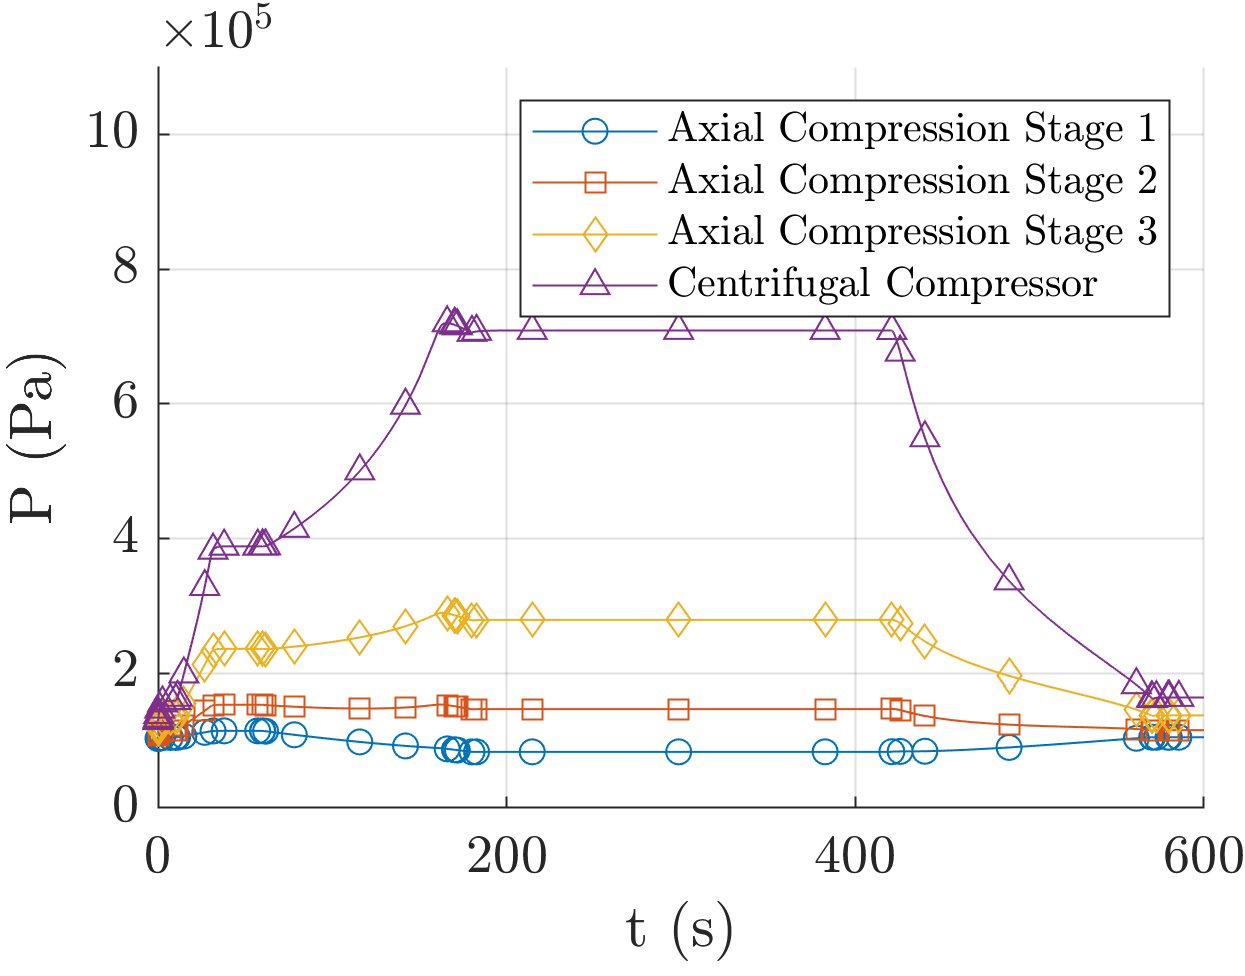
\includegraphics[width=\textwidth]{PREASSURE_TURBO_VALIDATION.png}
        \caption{Graph 1: Turboprop Engine Pressure}
        \label{fig:Pressuere_turbo_validation}
    \end{subfigure}
    \hspace{0.02\textwidth}
    \begin{subfigure}[b]{0.47\textwidth}
        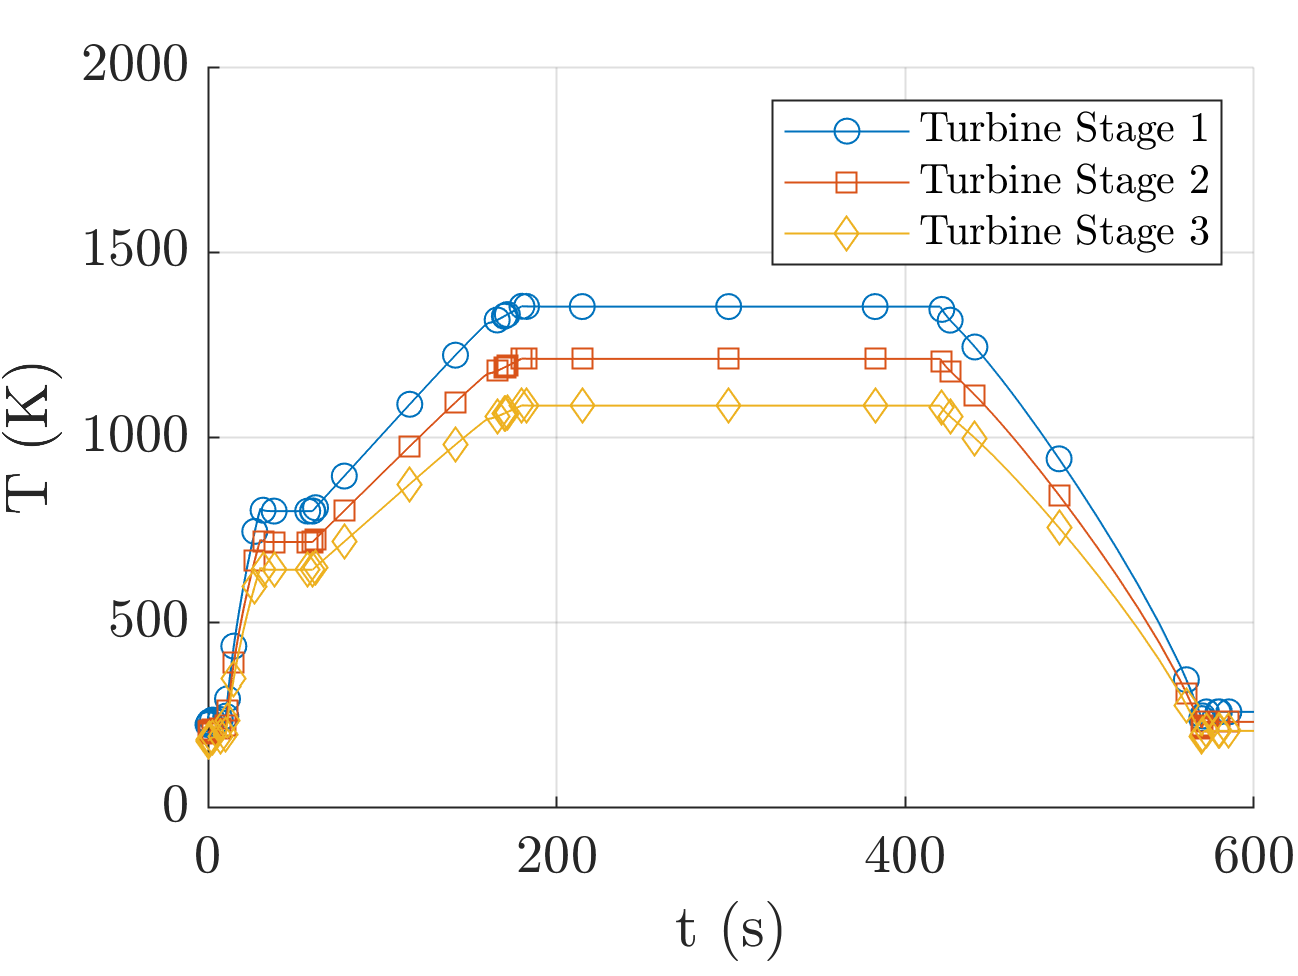
\includegraphics[width=\textwidth]{TEMPERATURE_TURBO_VALIDATION.png}
        \caption{Graph 2: Turboprop Engine Temperature}
        \label{fig:Temperature_turbo_validation}
    \end{subfigure}
    \vspace{15pt}
    \caption{Thermodynamic Turboprop Engine Results}
\label{fig:Pressuere_temperature_turbo_validation}
\end{figure}
For the analysis of the results, it is observed in \autoref{fig:Pressuere_turbo_validation} the pressures decrease and the temperatures increase in cruise conditions (from 180 sec to 420 sec) compared to \autoref{fig:P_compresion}. This trend is primarily due to the reduction in air density at higher altitudes, making it more challenging to achieve the same pressure levels as at sea level. Initially, we achieved pressures around 734,000 Pa, but under cruise conditions, the maximum pressure reached is approximately 650,000 Pa. Considering the baseline value of 780,000 Pa from ground-level tests, this represents an error of around 16. However, this discrepancy is not inaccurate; rather, it reflects the expected variation as air density decreases with altitude.

Similarly, the temperatures in \autoref{fig:Temperature_turbo_validation} show a significant increase compared to \autoref{fig:T_compresion} due to the reduced air-fuel ratio at higher altitudes. The observed temperature rises from 1,225 K to approximately 1,342 K. When compared to the baseline value of 1,212 K, this results in a 10 error. This variation is consistent with the anticipated thermal behavior under reduced air density conditions at higher altitudes.

In \autoref{fig:RPM_TURBO_VALIDATION}, the main RPM values for the turboprop engine system are shown, including the gas generation shaft, power generation shaft, and propeller RPMs. The gas generation shaft RPM initially increases rapidly and stabilizes around 45,000 RPM during steady-state operation, while the power generation shaft follows a similar trend, reaching a steady value of approximately 30,000 RPM. The propeller RPM, in contrast, remains much lower, reflecting the geared-down rotational speed necessary for propeller-driven propulsion. These RPM values confirm that the system remains within the engine's operational parameters \cite{Piper1998}, indicating that the integrated model is accurately representing expected behavior during typical flight conditions.

\begin{figure}[H]
    \centering
    {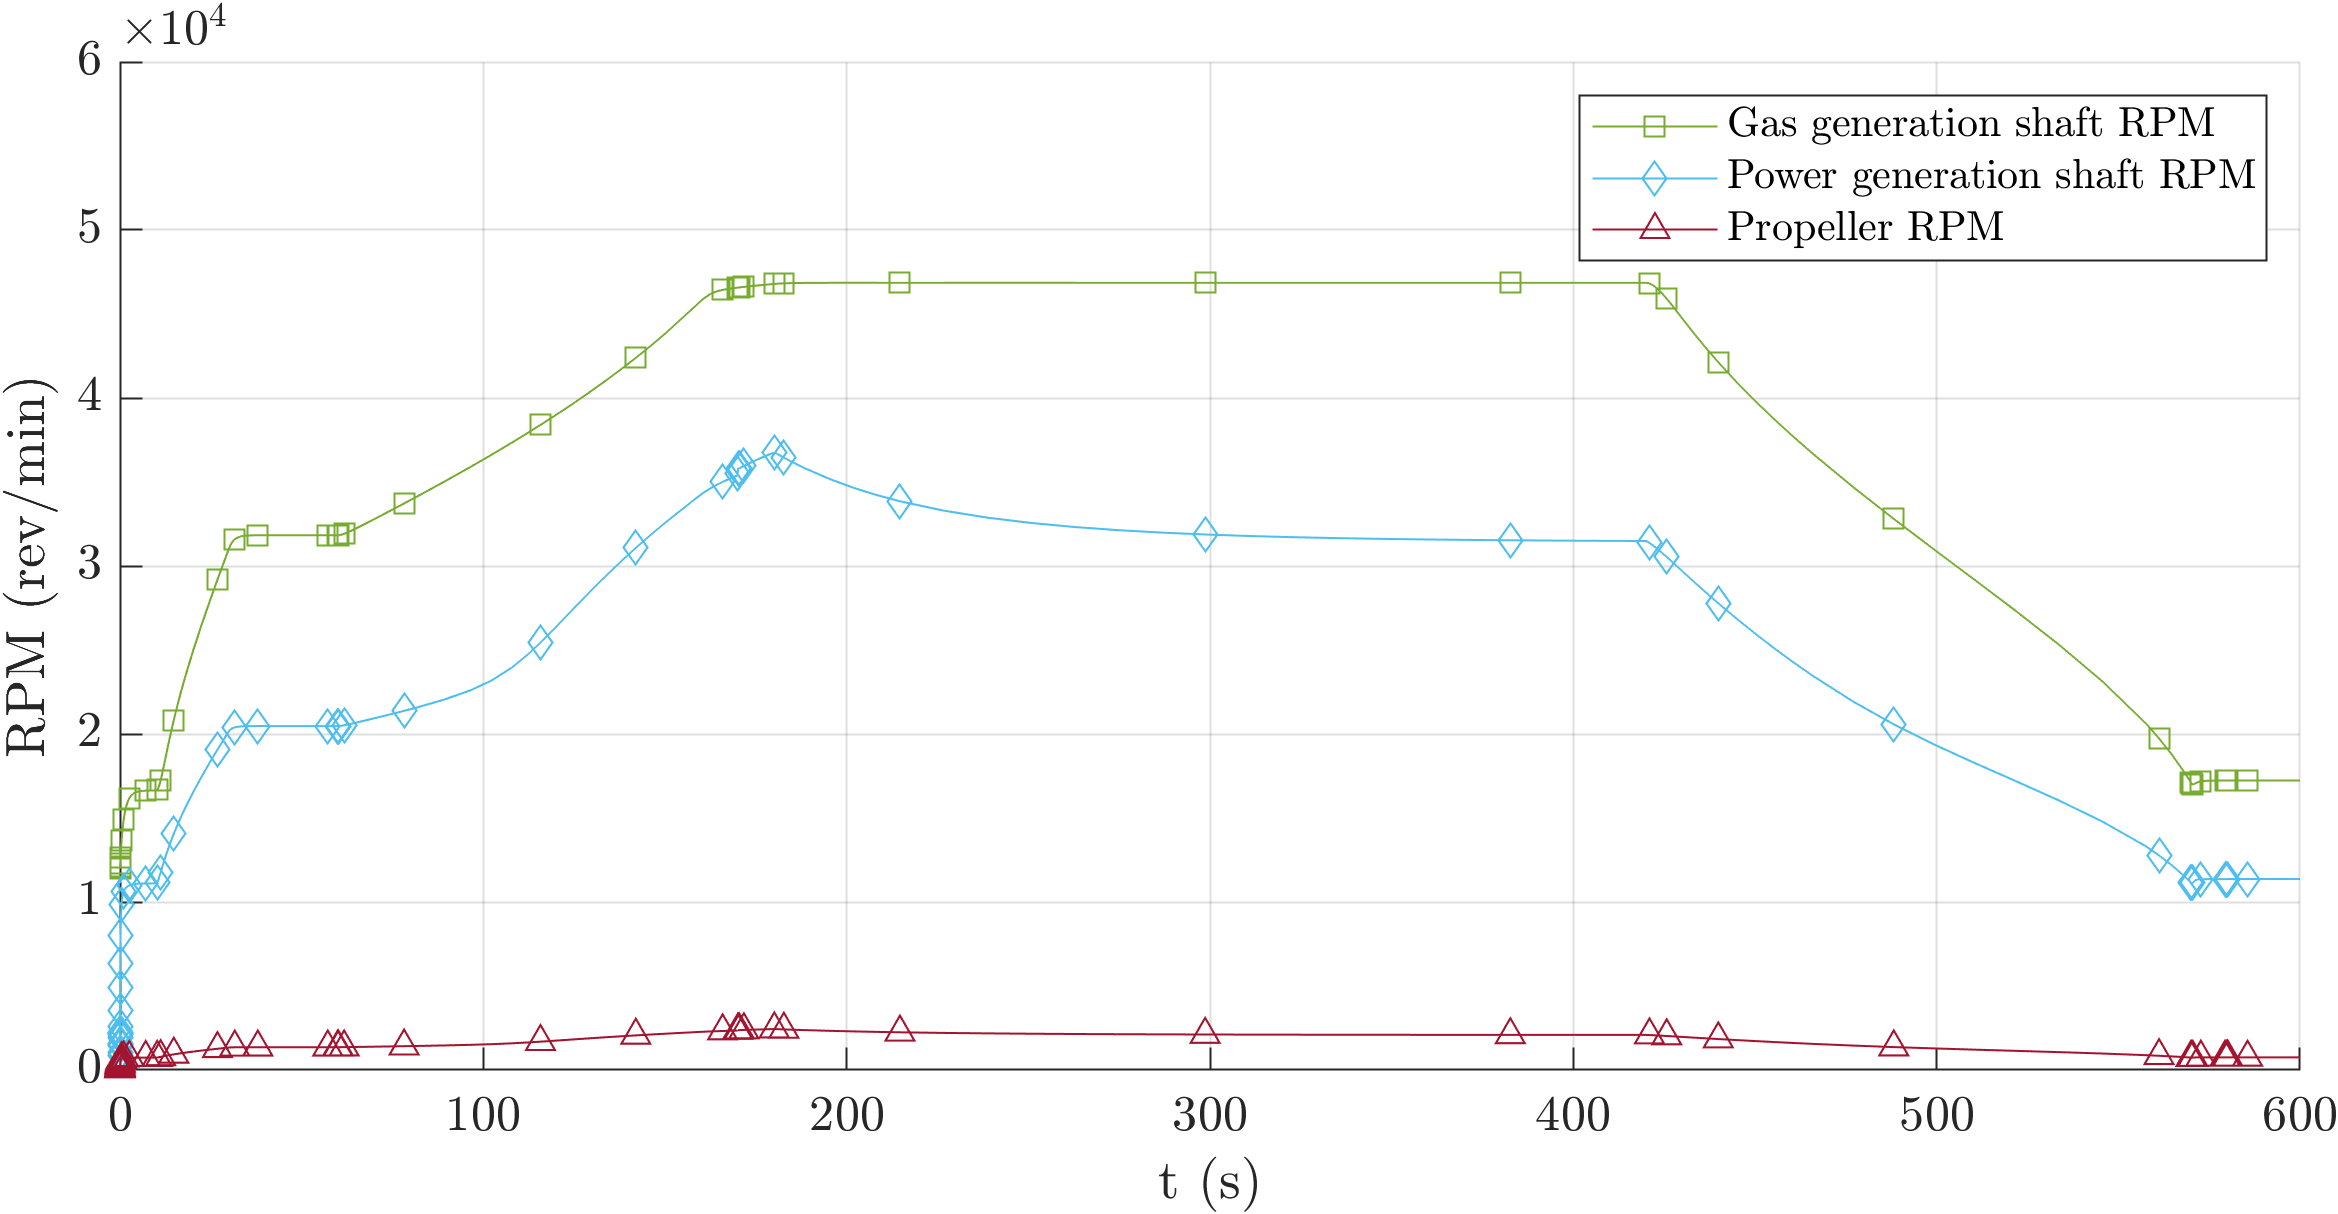
\includegraphics[width=0.70\textwidth]{RPM_turbo.png}}
    \caption{Main Turboprop RPMs Results}
    \label{fig:RPM_TURBO_VALIDATION}
\end{figure}

In the validation of torque data (\autoref{fig:TurboQ}), a trend consistent with the previous propeller validation analysis was observed. A significant aspect identified at this stage was the relationship between torque and RPM, mediated by the pitch angle. During takeoff, the pitch angle is adjusted to allow an increase in RPM, which generates a temporary decrease in torque due to a reduction in aerodynamic resistance faced by the propeller. This configuration favors the initial acceleration of the engine, while in the cruise phase, the system stabilizes in a balance between torque and RPM \cite{book:96630002}. It is noteworthy that torque values remained below the operational limit of 3086 N.m, ensuring that the model complies with safety margins and preserves its fidelity under real operating conditions.

Regarding thrust (\autoref{fig:TurboT}), a similar response to the trend described in the initial propeller validation was observed. However, in this case, thrust values appear reduced due to the interaction with the aircraft's speed, an intrinsic phenomenon in thrust behavior. As the aircraft increases its speed, the relative airflow decreases the propeller's efficiency, reducing the pressure differential and increasing drag on the blades, thereby decreasing net thrust \cite{book:96630002,stengel2024power} It is important to note that values shown in the graphs may be somewhat elevated, as this analysis focuses on engine, excluding aerodynamic forces and aircraft weight, factors that would further reduce these values under real flight conditions.


\begin{figure}[h]
    \centering
    \begin{subfigure}[b]{0.47\textwidth}
        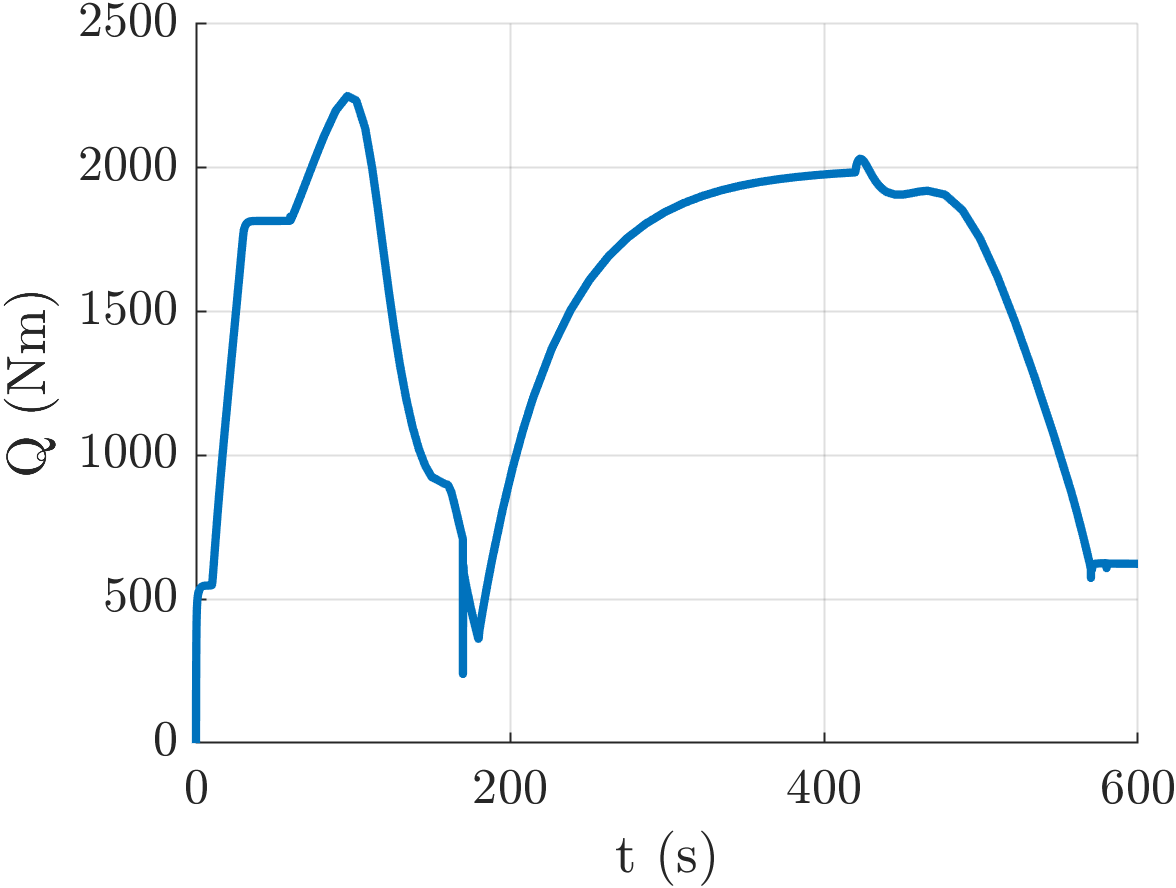
\includegraphics[width=\textwidth]{T_TURBO_VALLIDATION.png}
        \caption{Graph 1: Turboprop Torque}
        \label{fig:TurboQ}
    \end{subfigure}
    \hspace{0.02\textwidth}
    \begin{subfigure}[b]{0.47\textwidth}
        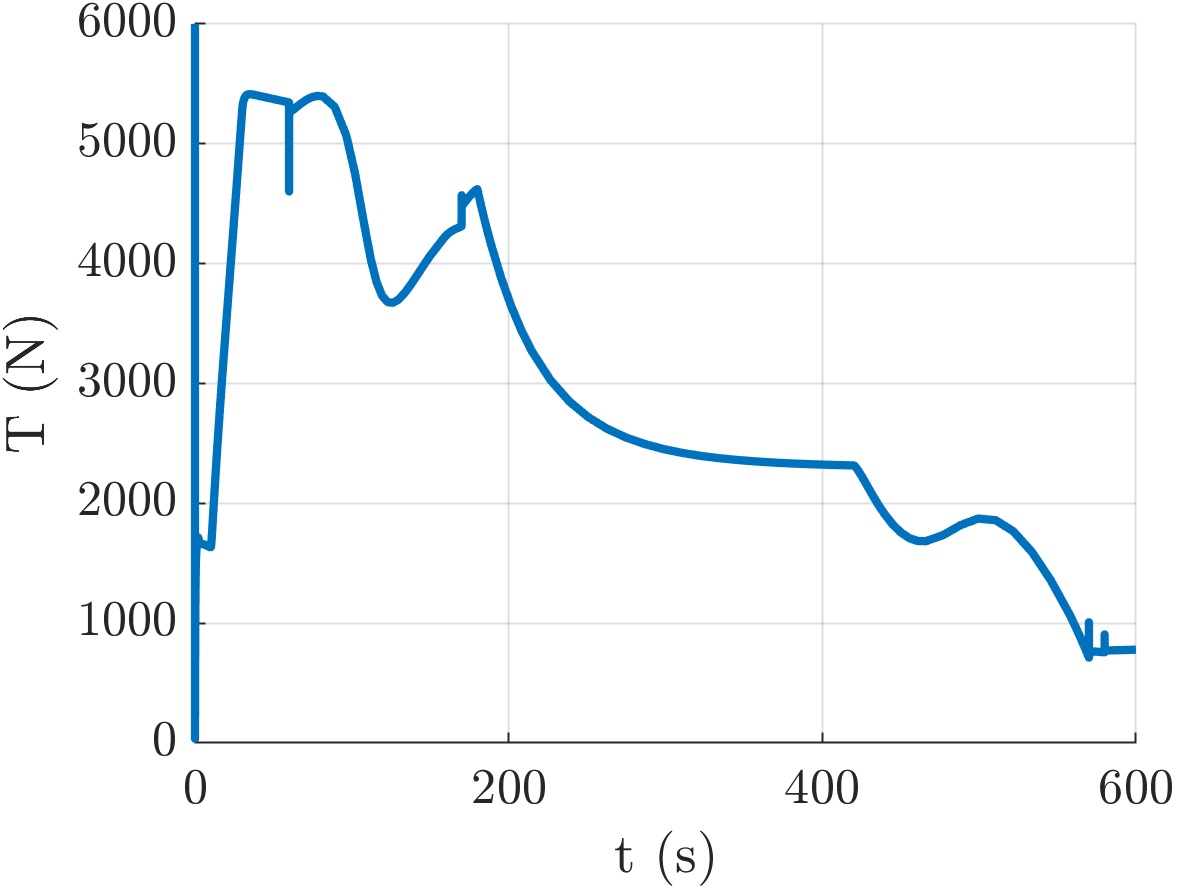
\includegraphics[width=\textwidth]{Q_TURBO_VALLIDATION.png}
        \caption{Graph 2:Turboprop Thrust}
        \label{fig:TurboT}
    \end{subfigure}
    %\vskip\baselineskip
    \vspace{15pt}
    \caption{Aerodynamic Turboprop Propeller Results}
    \label{fig:TurboTQ}
\end{figure}

The thermal efficiency observed in \autoref{fig:Turboprop_Efficiency} throughout the simulation reflects the inherent characteristics of a gas turbine cycle. The thermal efficiency, calculated as in equation \ref{eq:Thermal_Tuboprop_Efficiency} based on \cite{book:96630002}, the gas shaft power divided by the heat power, yields an average value of around 40\% at operation stages (take off, cruise and descend) between 60 sec to 430 sec, which resembles the analysis by \cite{pulido2008conversión} on Brayton turbomachinery under real operating conditions. It's important to note that this calculation excludes the power from the first turbine stage, as that energy is directed entirely towards the compression stage and does not contribute directly to propeller movement. This division aligns with the fundamental design of turboprop engines, where a portion of the energy is dedicated to sustaining the compression cycle rather than propulsion.



\begin{figure}[h]
    \centering
    \begin{subfigure}[b]{0.33\textwidth}
        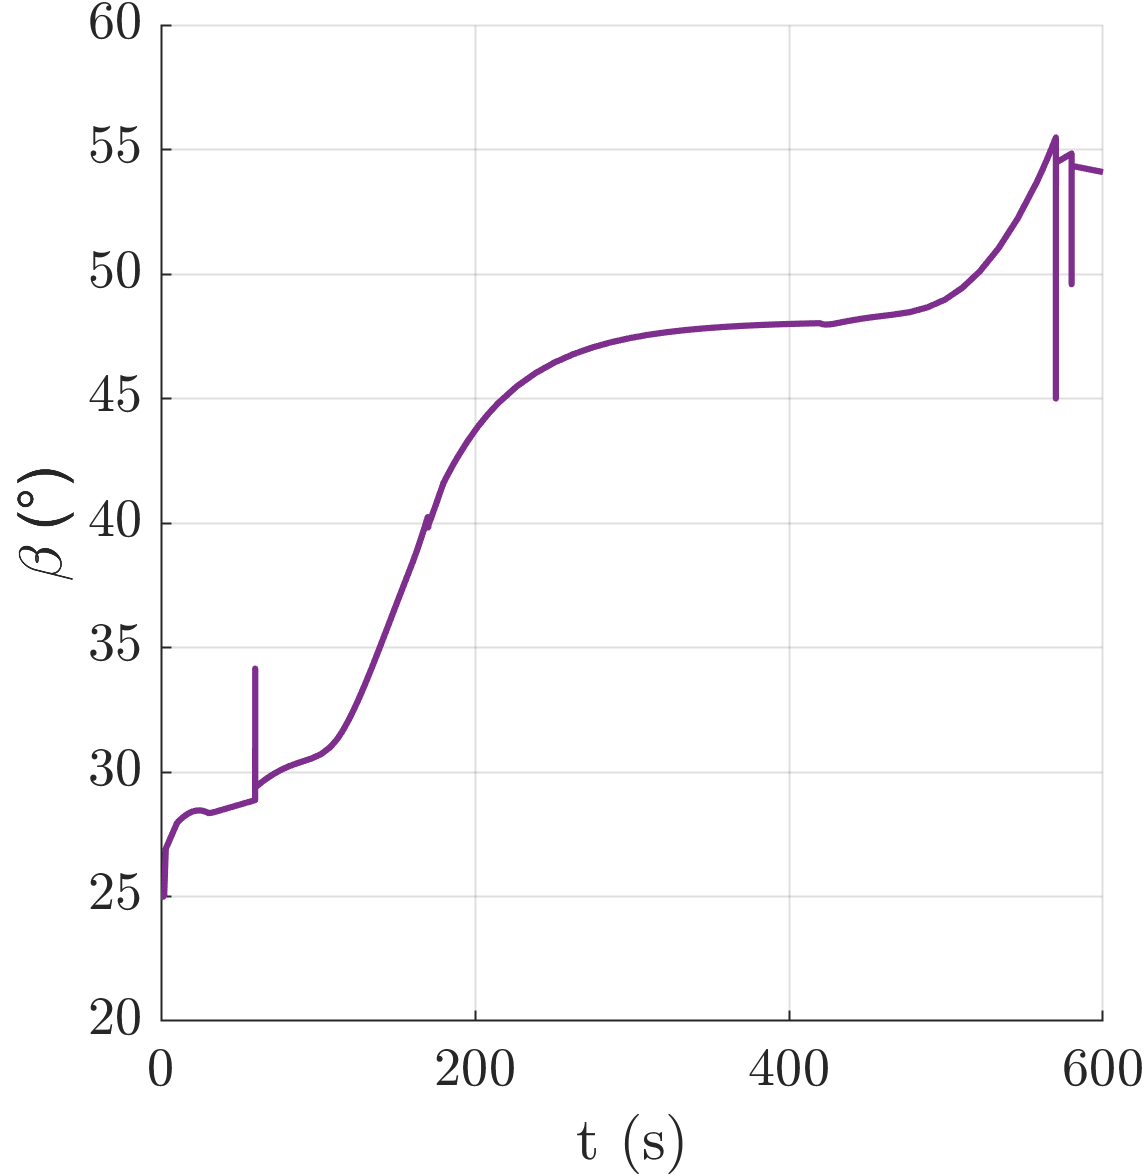
\includegraphics[width=\textwidth]{n_beta - copia.png}
        \caption{Turboprop Pitch Angle Results}
        \label{fig:Turboprop_Pitch_Angle}
    \end{subfigure}    
    \hspace{0.05\textwidth}
    \begin{subfigure}[b]{0.4\textwidth}
        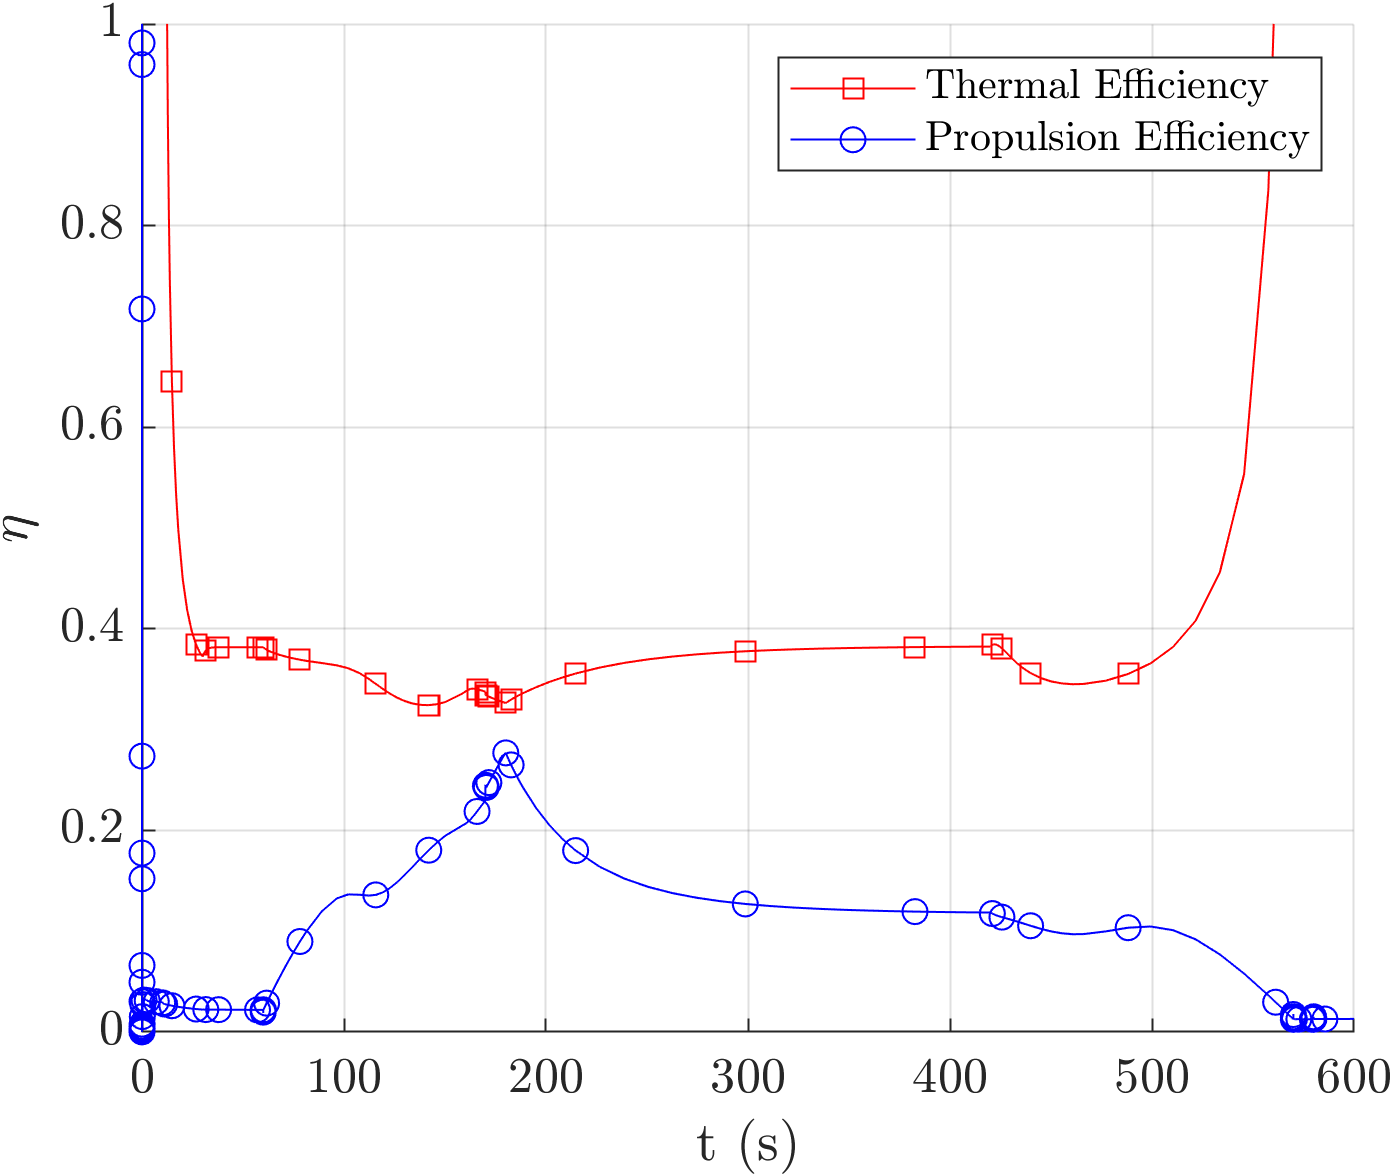
\includegraphics[width=\textwidth]{n_beta.png}
        \caption{Turboprop Efficiency Results}
        \label{fig:Turboprop_Efficiency}
    \end{subfigure}
    %\vskip\baselineskip
    \vspace{15pt}
    \caption{Turboprop Efficiency and Pitch Angle Results}
    \label{fig:Turboprop_Efficiency_Pitch Angle}
\end{figure}

\begin{equation}\label{eq:Thermal_Tuboprop_Efficiency}
    \eta_{T} = \frac{\dot{W}^{t_2}+\dot{W}^{t_3}}{\dot{m}_{f}LHV}
\end{equation}


Interestingly, efficiency values greater than 100\% appear both at the beginning and end of the simulation in \autoref{fig:Turboprop_Efficiency} due to specific operational scenarios. Initially, this elevated efficiency results from simulating an external power source (like a battery) that powers the turbine to reach minimum operational conditions before fuel injection begins, meaning the turbine’s power does not yet rely on fuel combustion. Similarly, during the descent phase, the shaft inertia maintains turbine output as fuel injection decreases, producing another peak in efficiency. These values highlight the dynamic nature of the engine and represent transient conditions rather than actual efficiencies.
\begin{equation}\label{eq:Propulsion_Tuboprop_Efficiency}
    \eta_{P} = \frac{TV_{\infty}}{\dot{W}^{t_2}+\dot{W}^{t_3}}
\end{equation}

In the analysis of the propulsion efficiency calculated as in equation \ref{eq:Propulsion_Tuboprop_Efficiency} based on \cite{book:96630002}, which means Propeller power divided by gas shaft power; certain limitations related to the aircraft's flight speed (\( V_\infty \)) were identified. Although the operational parameters allowed for higher speeds, under the Traub model the aircraft did not exceed 60 m/s, resulting in a low advance ratio (\( J \)) of approximately 0.15. As \cite {book:96630002} mentions, propulsion efficiency depends greatly on the aircraft's speed and, consequently, on its advance ratio. In this case, the engine had the capacity to deliver greater power, but the speed achieved was insufficient to support a high \( J \) value, leading to a reduction in propulsion efficiency. 

\begin{table}[h!]
    \centering
    \begin{tabular}{|c|c|c|c|}
        \hline
        \textbf{J} & \textbf{$C_T$} & \textbf{$C_P$} & \textbf{$\eta$} \\
        \hline
        0.3142 & 0.1250 & 0.0734 & 0.535 \\
        0.4398 & 0.1077 & 0.0710 & 0.667 \\
        0.5655 & 0.0898 & 0.0674 & 0.754 \\
        0.6912 & 0.0703 & 0.0596 & 0.815 \\
        0.8168 & 0.0497 & 0.0475 & 0.854 \\
        0.9425 & 0.0278 & 0.0306 & 0.856 \\
        \hline
    \end{tabular}
    \vspace{10pt}
    \caption{Typical propeller efficiency table including $J$, $C_T$, $C_P$, and $\eta$ \cite{book:96630002}.}
    \label{tab:propeller_efficiency}
\end{table}

To support the observed efficiency value, Gudmundsson's table (\autoref{tab:propeller_efficiency}) of propulsion efficiency at different advance ratios was used as a reference. From the table data, a quadratic regression of these values was performed, resulting in a graph that shows a generalization of the values of \( C_P \), \( C_T \), and \( \eta \) for any \( J \) between 0 and 1 as seen in \autoref{fig:GUD_prop}. With the value \( J = 0.15 \) obtained in the simulation, this data was substituted into the regression obtained for propulsive efficiency, yielding a value of 
 \( \eta \) = 0.33. Comparing this value with the one obtained from the simulation (\( \eta \) = 0.27), an error of 18\,\% was observed, which is attributed firstly to the fact that the values developed by Gudmundsson correspond to a diameter 0.0237 meters smaller than the one used in the simulation, and secondly to the problems found with the air velocity that are assumed to affect all stages of the simulation. However, it is not a value too far from what was desired, indicating a good start for future studies.

\begin{figure}[H]
\centering
    \begin{minipage}{0.55\textwidth}
        \centering
        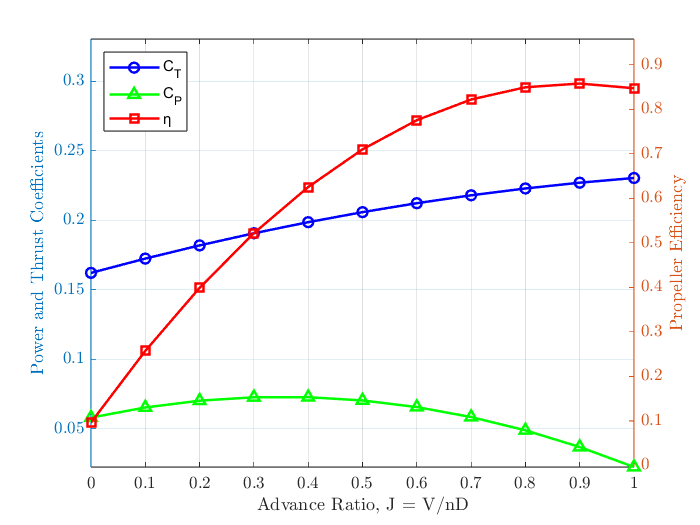
\includegraphics[width=\textwidth]{gudmundsson_imagen.png}
        \caption{Typical propeller efficiency graph for a fix pitch propeller (no specific propeller type) \cite{book:96630002}}
        \label{fig:GUD_prop}
    \end{minipage}
\end{figure}

The PID control shown in \autoref{fig:Turboprop_Pitch_Angle} implemented in Simulink effectively regulated the pitch angle by targeting a specified torque range based on values established in \cite{Castellanos2023Propeller}. This approach provided a more responsive regulation of RPMs compared to a predefined pitch angle schedule, allowing the engine to reach the desired RPMs more efficiently. Additionally, since the system could dynamically adjust, the PID adapted the pitch angle within the expected range as flight conditions varied, such as changes in altitude or airspeed. Although the control performed well under standard conditions, a limitation emerged at very high airspeeds, where torque would drop, prompting the PID to seek higher pitch angles. While this did not push the system into feathering range (pitch angles over 75°), the pitch angle occasionally exceeded 48°, which was higher than the range specified in \cite{Castellanos2023Propeller}.



% \begin{figure}[h]
%     \centering
%     \begin{subfigure}[b]{0.8\textwidth}
%         \centering
%         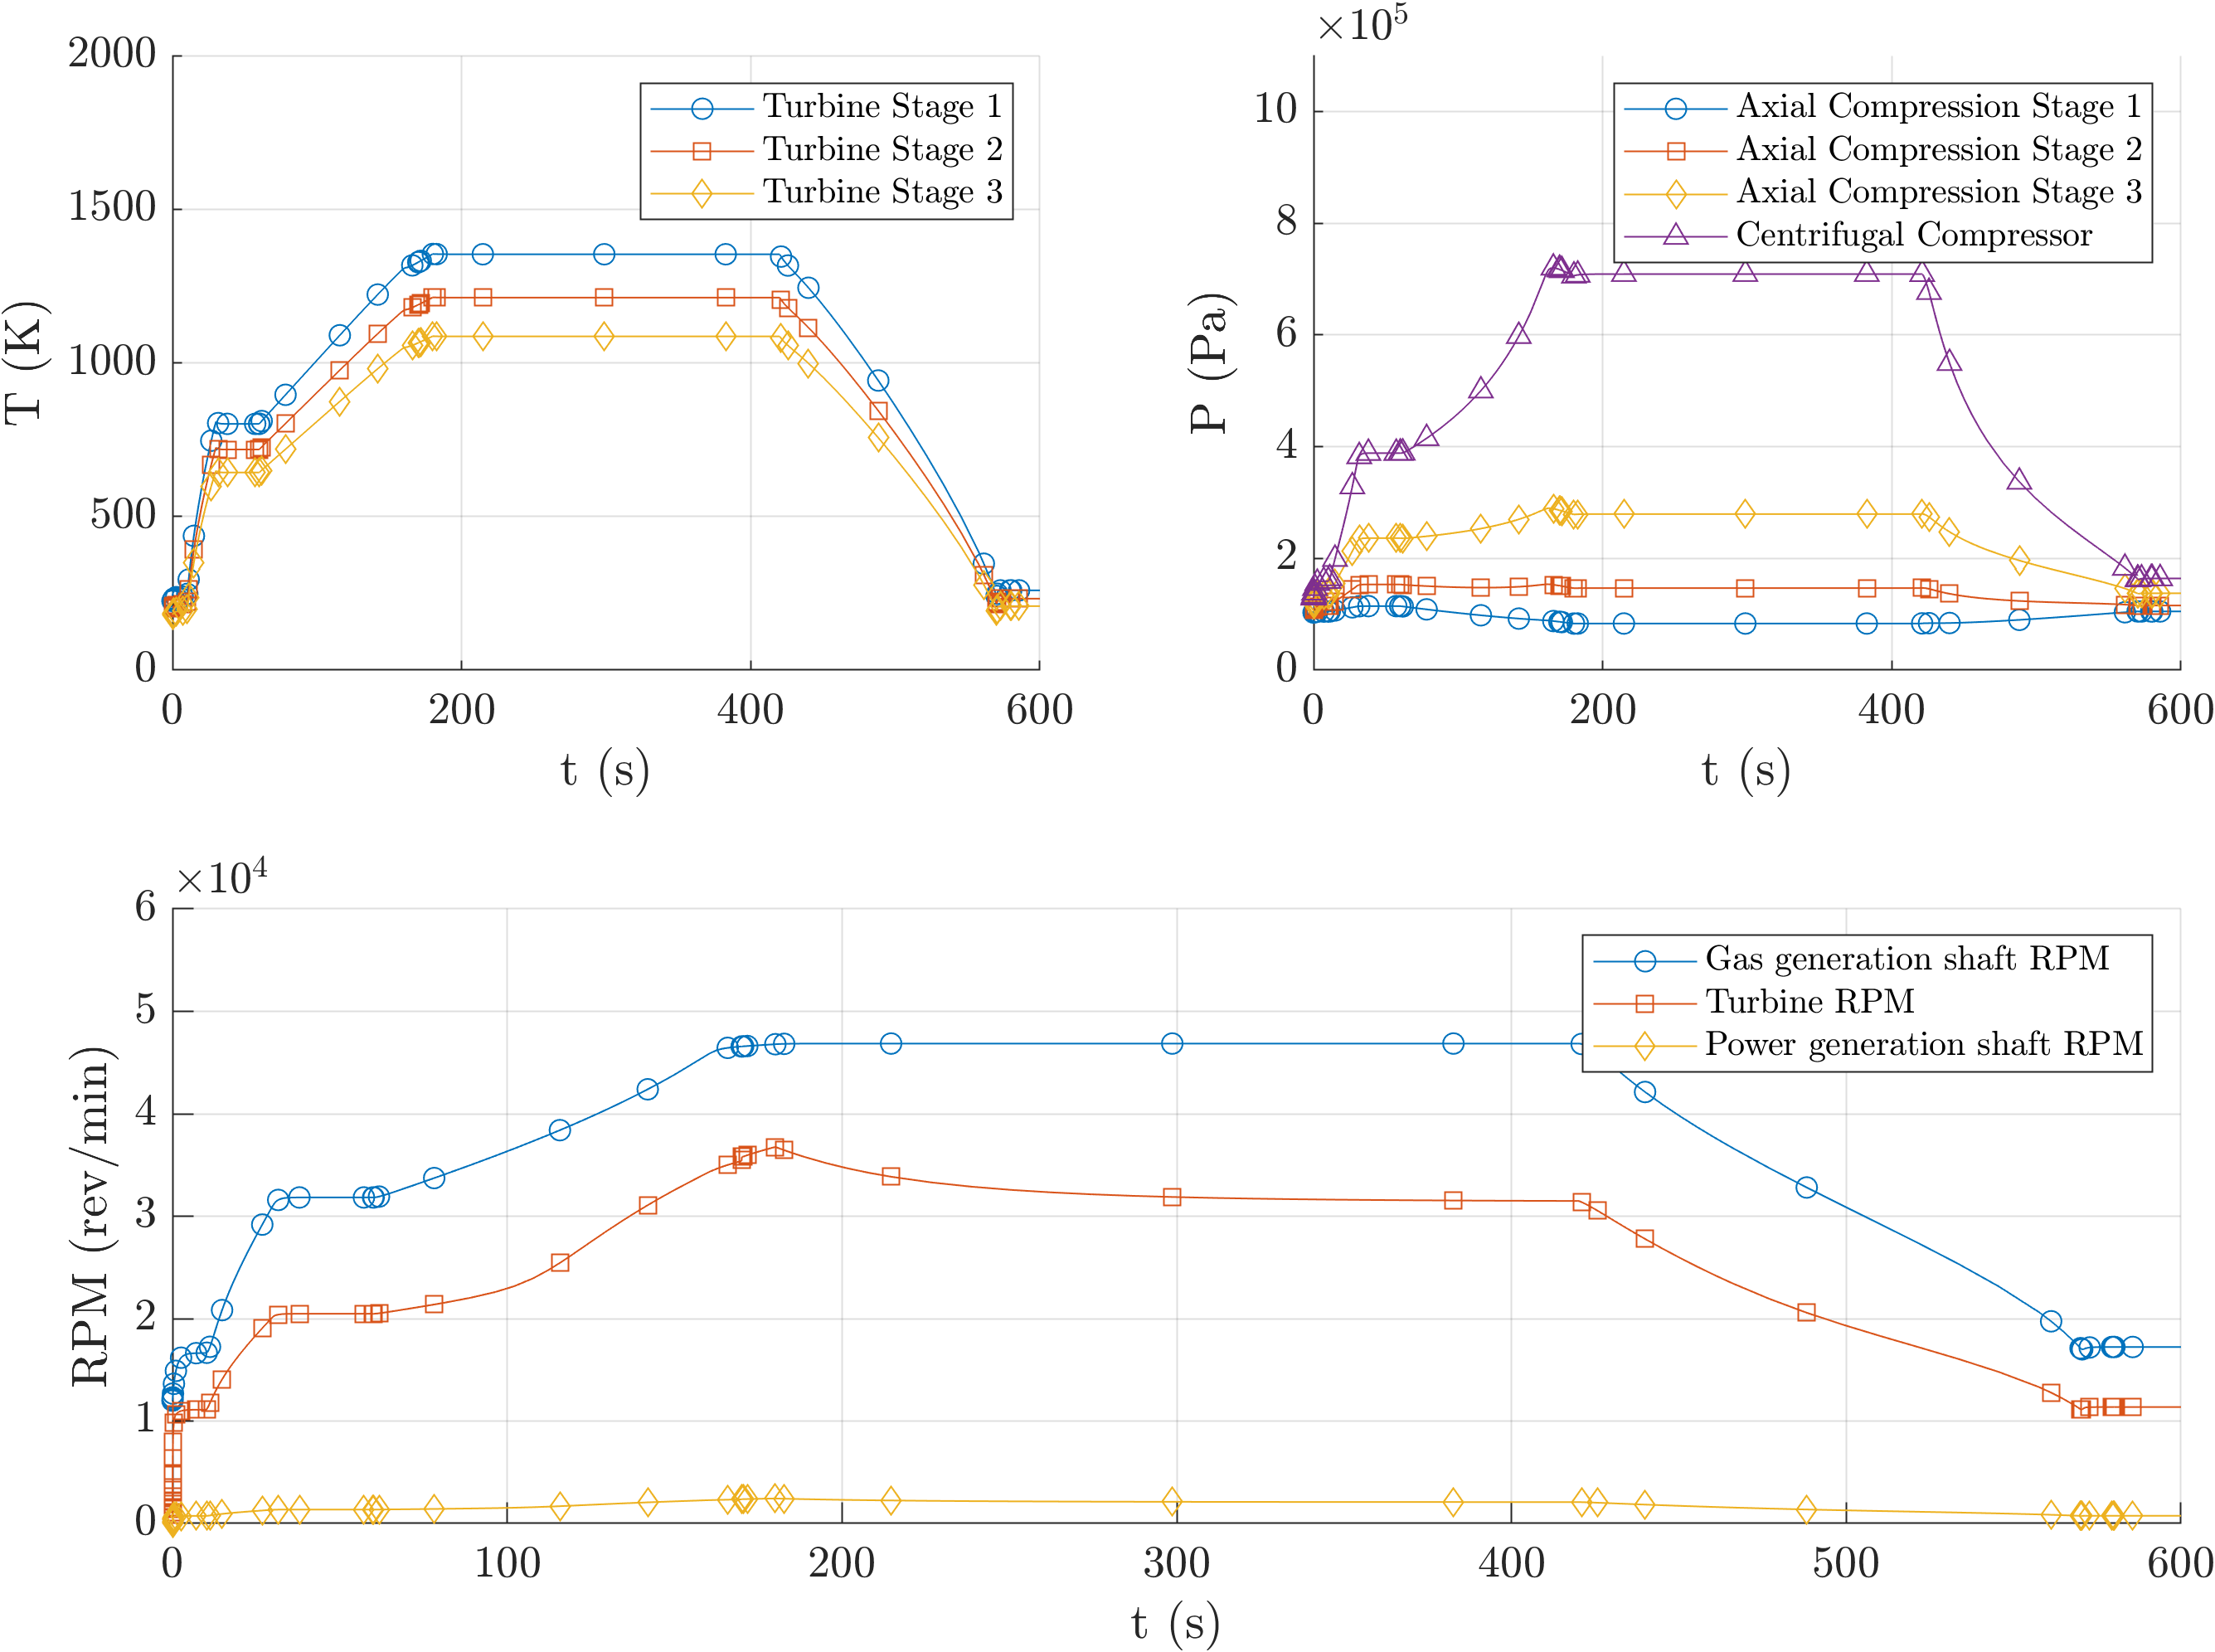
\includegraphics[width=\textwidth]{full_turbo.png}
%         \caption{Graph 1: Compression Stage Pressure and Temperature}
%         \label{fig:DeftStatic}
%     \end{subfigure}
%     \vskip\baselineskip % Espacio entre las dos imágenes
%     \begin{subfigure}[b]{0.8\textwidth}
%         \centering
%         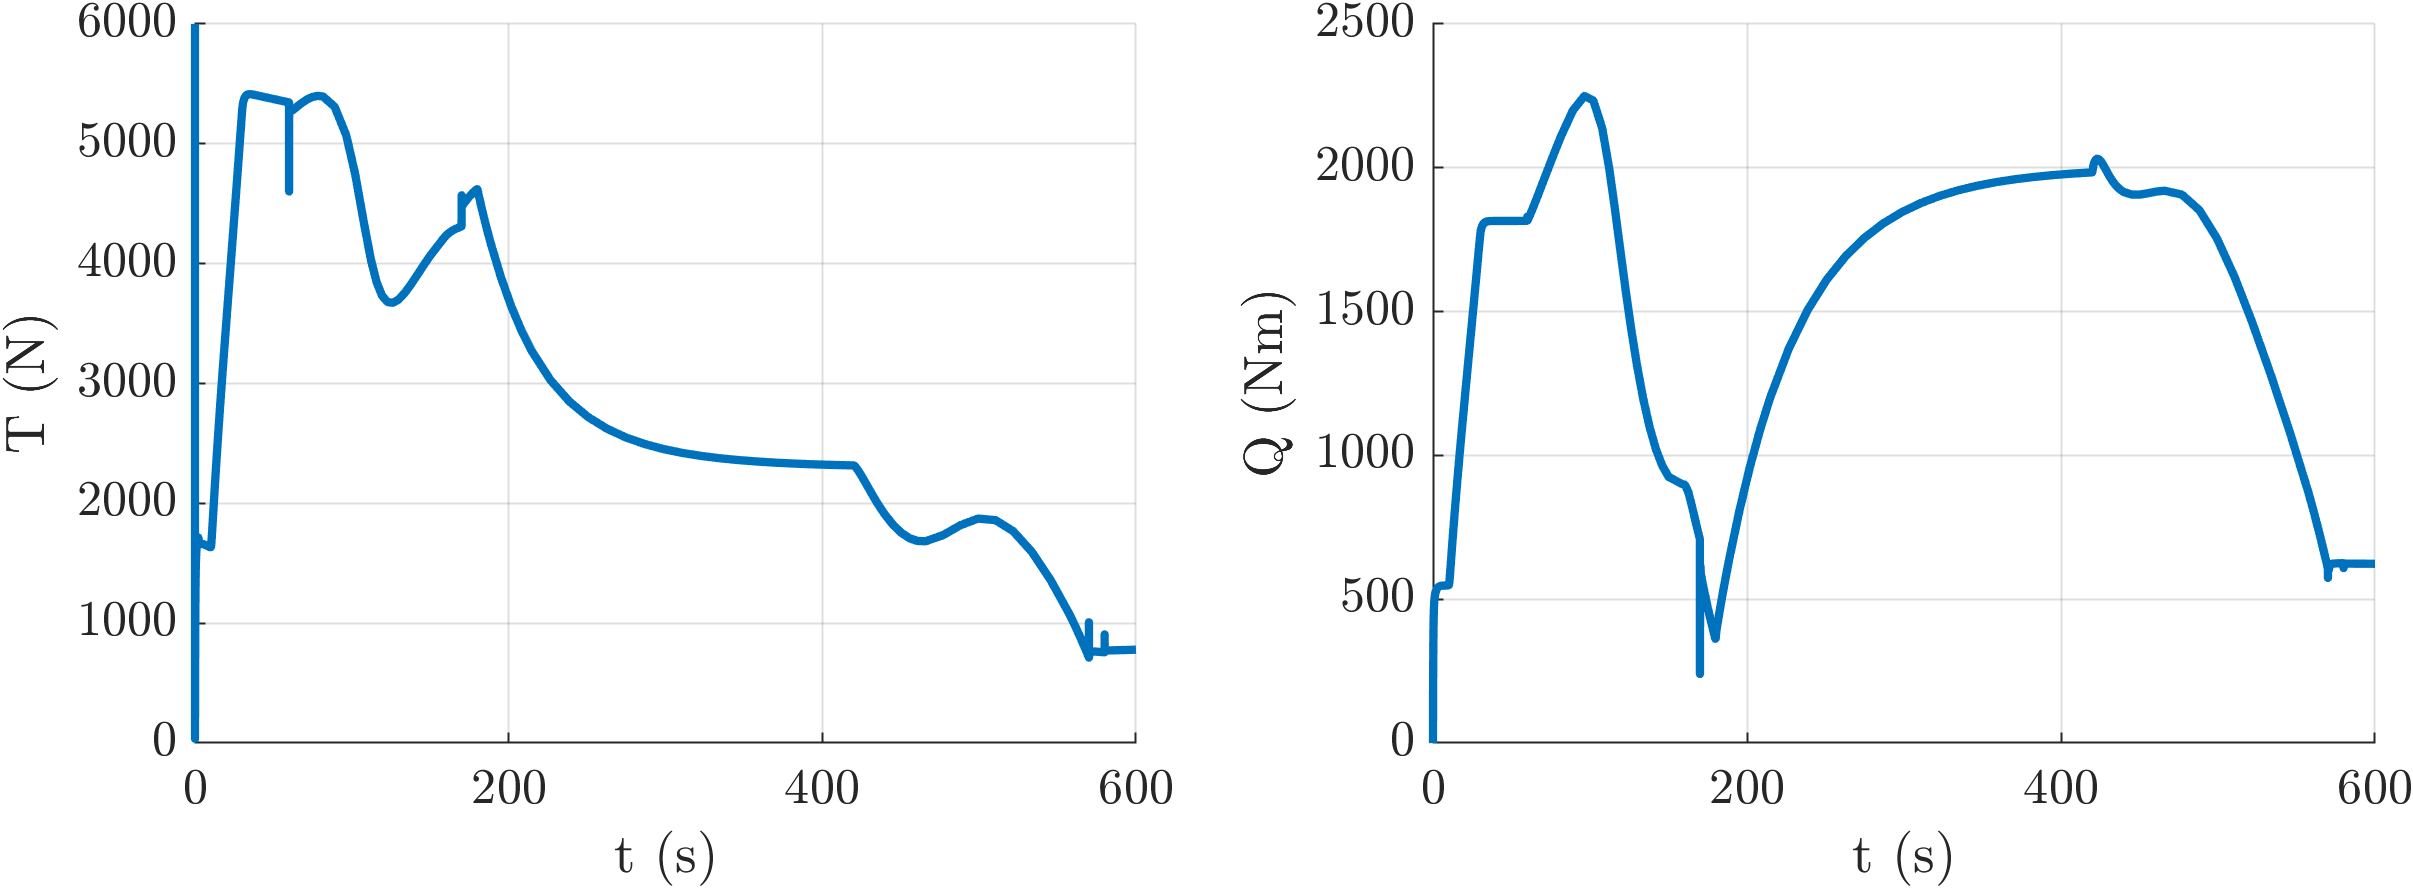
\includegraphics[width=\textwidth]{T_Q_turbo.png}
%         \caption{Graph 2: Turbine Stage Pressure and Temperature}
%         \label{fig:TSFCStatic}
%     \end{subfigure}
%     \caption{Engine Simulation Results}
%     \label{fig:comparisonStatic}
% \end{figure}


\section{Simulation Section: \emph{To simulate the aerothermodynamic operation of the Turboprop engine in idle, taxiing, takeoff, and cruise regimes, operating with different conventional and alternative fuels.}}\label{sec:Method}

To address modern environmental challenges, this last study explores the feasibility of employing Sustainable Aviation Fuels (SAF) and non-conventional energy resources (NCER) in the aviation sector, particularly within turboprop engine applications. By assessing various blends of Jet A1 and biodiesel, we aim to evaluate the impact of these alternative fuels on the thermal and propulsive behavior of the engine.

\subsection{Fuel Blend Configurations}
Assessing the feasibility of Jet A1 and biodiesel blends in aviation, the lower heating values (LHVs) were calculated for three specific fuel mixtures: 100\% Jet A1, 75/25 Jet A1-biodiesel, and 50/50 Jet A1-biodiesel. The LHV for each blend was determined using a weighted average of the individual LHVs of Jet A1 and biodiesel, based on their respective mass fractions. The formula used is as follows:

\begin{equation}
    \text{LHV}_{\text{blend}} = x ( \text{LHV}_{\text{Jet A1}}) + y ( \text{LHV}_{\text{biodiesel}})
\end{equation}

where \( x \) and \( y \) denote the mass fractions of Jet A1 and biodiesel, respectively. For this analysis, the values used were \(\text{LHV}_{\text{Jet A1}} = 43.1 \, \text{MJ/kg}\) \cite{A1specs2018} and \(\text{LHV}_{\text{biodiesel}} = 37.52 \, \text{MJ/kg}\) \cite{Mehta2009LHV}. The calculated LHVs for each blend are presented in the \autoref{table:LHV_total}:


\begin{table}[h!]
\centering
\renewcommand{\arraystretch}{1.2} % Espaciado entre filas
\begin{tabular}{@{}ccc@{}}
\toprule
\textbf{Jet Fuel A1 (\%)} & \textbf{Biodiesel (\%)} & \textbf{LHV Total (MJ/kg)} \\ \midrule
100                       & 0                       & 43.20   \\
75                        & 25                      & 41.78   \\
50                        & 50                      & 40.36   \\ \bottomrule
\end{tabular}
\vspace{10pt}
\caption{LHV Total for Different Combinations of Jet Fuel A1 and Biodiesel}
\label{table:LHV_total}
\end{table}

Using the new LHV values for various proportions of Jet Fuel A1 and Biodiesel, an analysis will be conducted to assess the impact of each mixture on all validation parameters, focusing on potential effects on engine power output and overall operational efficiency.


\subsection{Blends Performance Evaluation}

Below, the results for the different fuel mixtures will be presented in order to contrast their main characteristics. The legend for the graphs can be found in \autoref{tab:legend}.

\begin{table}[h!]
\centering
\renewcommand{\arraystretch}{1.2} % Adjust vertical spacing between rows
\begin{tabular}{@{}>{\centering\arraybackslash}m{1.5cm} @{}>{\centering\arraybackslash}m{3cm}@{}}
\toprule
\textbf{Notation} & \textbf{Fuel Combination} \\ \midrule
\raisebox{-.3\height}{%
    
\begin{tikzpicture}
        \draw[green, thick] (-0.1,-0.1) rectangle (0.1,0.1); % Smaller green square
    \end{tikzpicture}
} & JA1 100\% \\
\raisebox{-.3\height}{%
    
\begin{tikzpicture}
        \draw[cyan, thick] (0,-0.14) -- (0.14,0) -- (0,0.14) -- (-0.14,0) -- cycle; % Adjusted cyan diamond
    \end{tikzpicture}
} & JA1 75\%  \\
\raisebox{-.3\height}{%
    
\begin{tikzpicture}
        \draw[red, thick] (-0.1,-0.1) -- (0.1,-0.1) -- (0,0.1) -- cycle; % Smaller red triangle
    \end{tikzpicture}
} & JA1 50\% \\ \bottomrule
\end{tabular}
\vspace{10pt}
\caption{Fuel Notation in Plots}
\label{tab:legend}
\end{table}


The following graphs illustrate the impact of Jet A1 and biodiesel blends on key variables for machinery integrity, such as pressure (\autoref{fig:P_cent_turbo}) and temperature(\autoref{fig:T_turb_turbo}), as well as performance metrics, including thrust (\autoref{fig:thrust_T}) and efficiencies (propulsive in \autoref{fig:propulsive_efficiency} and thermal in \autoref{fig:thermal_efficiency}) during the different flight phases. These results highlight the thermal and mechanical performance differences between each fuel.

During the pressure analysis, it was observed  in \autoref{fig:P_cent_turbo} that the values recorded for the various blends remained below the operational limit of 730 kPa. This behavior is primarily attributed to the reduced torque output generated by the alternative fuels, particularly in the blend with the lowest LHV (50/50), which showed an 18\% reduction compared to Jet A1. This difference becomes more pronounced during the cruise phase (from 180 sec to 420 sec), where the engine operates at its maximum efficiency for an extended period. In contrast, during the takeoff, \textit{idle}, and \textit{taxiing} phases, the pressure differences between the blends were less significant, as these phases do not require continuous high engine performance.

Regarding temperature (see \autoref{fig:T_turb_turbo}), the values obtained for Jet A1 and the blends exhibited minimal differences compared to \autoref{fig:Temperature_turbo_validation} and \autoref{fig:T_compresion}, particularly during the cruise phase, where the maximum values ranged between 1300 K and 1320 K. This slight increase during cruise can be attributed to operational factors related to altitude. Across other flight phases, the temperature differences between the blends remained consistent, with a maximum deviation not exceeding 35 K. This suggests that the combustion process, although influenced by the LHV of each blend, maintains stable thermal behavior across all evaluated fuels.
% Primera fila: presión y temperatura
\begin{figure}[H]
\centering
    \begin{minipage}{0.45\textwidth}
        \centering
        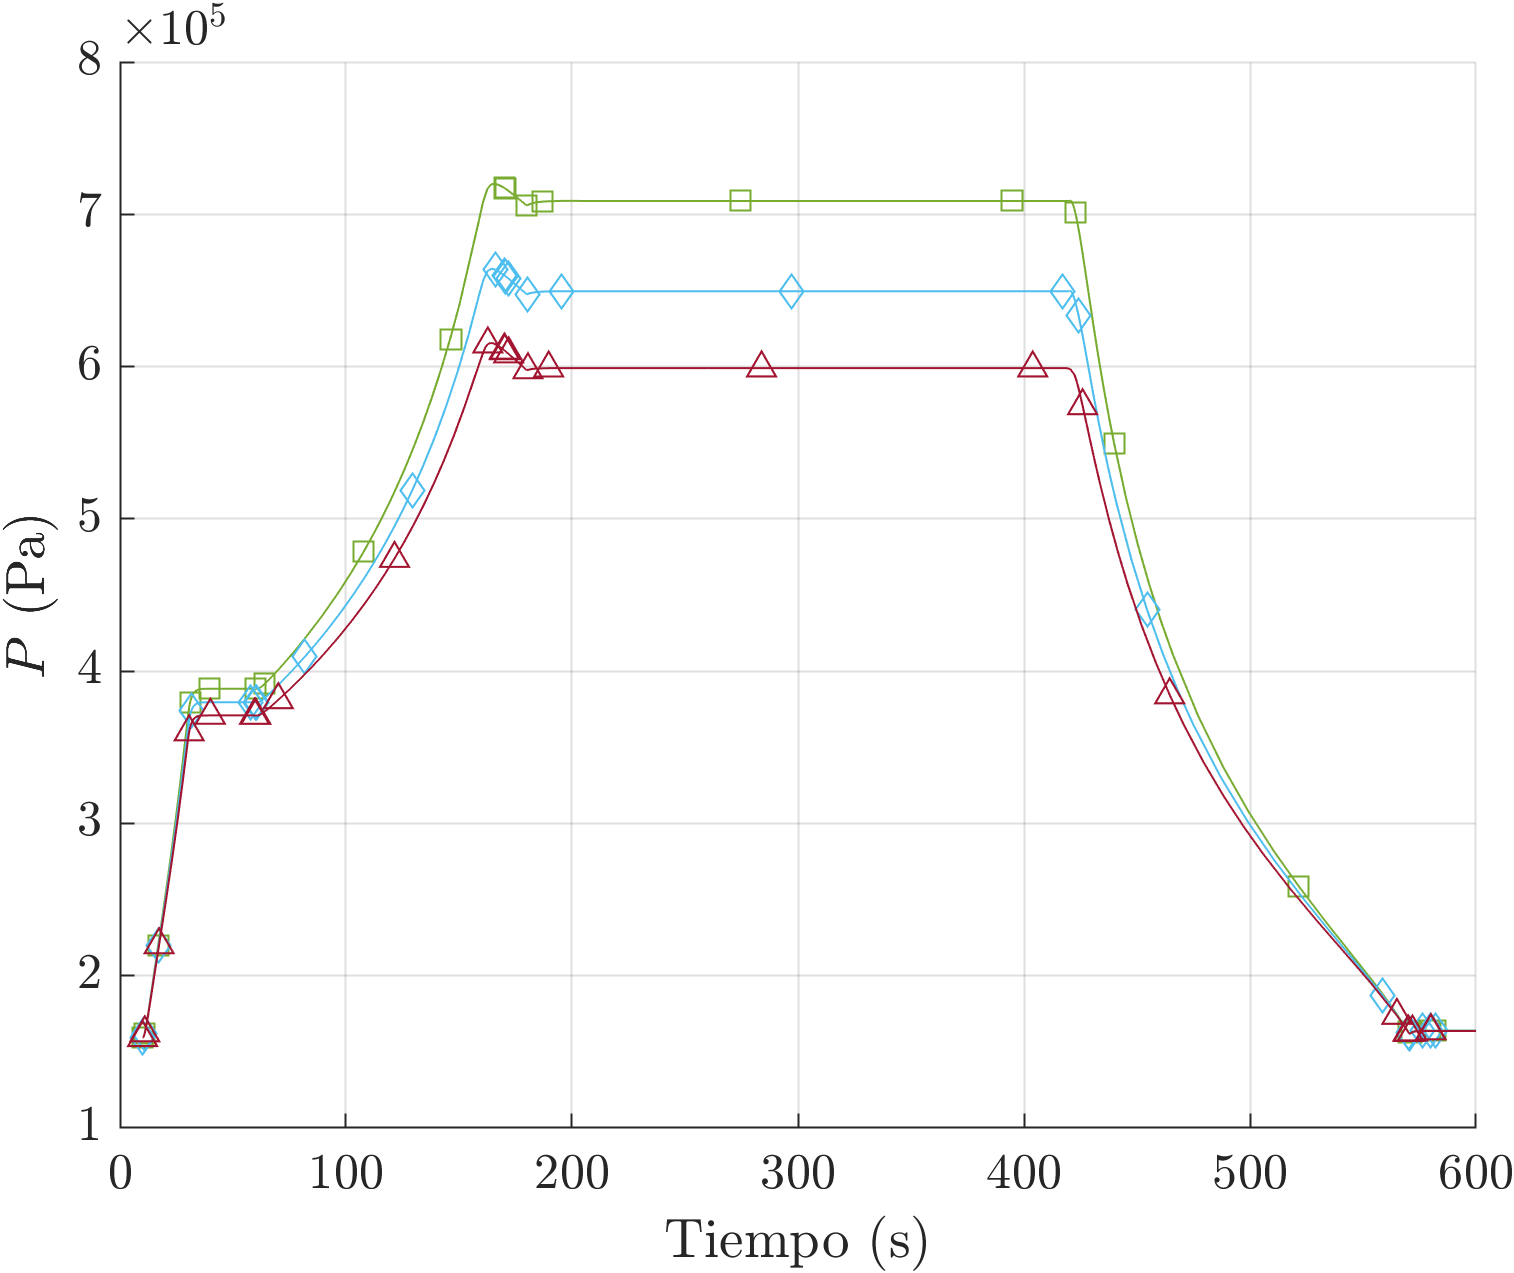
\includegraphics[width=\textwidth]{grafica_P_cent_combustibles.png}
        \caption{Compression stage pressure}
        \label{fig:P_cent_turbo}
    \end{minipage}
    \hfill
    \begin{minipage}{0.45\textwidth}
        \centering
        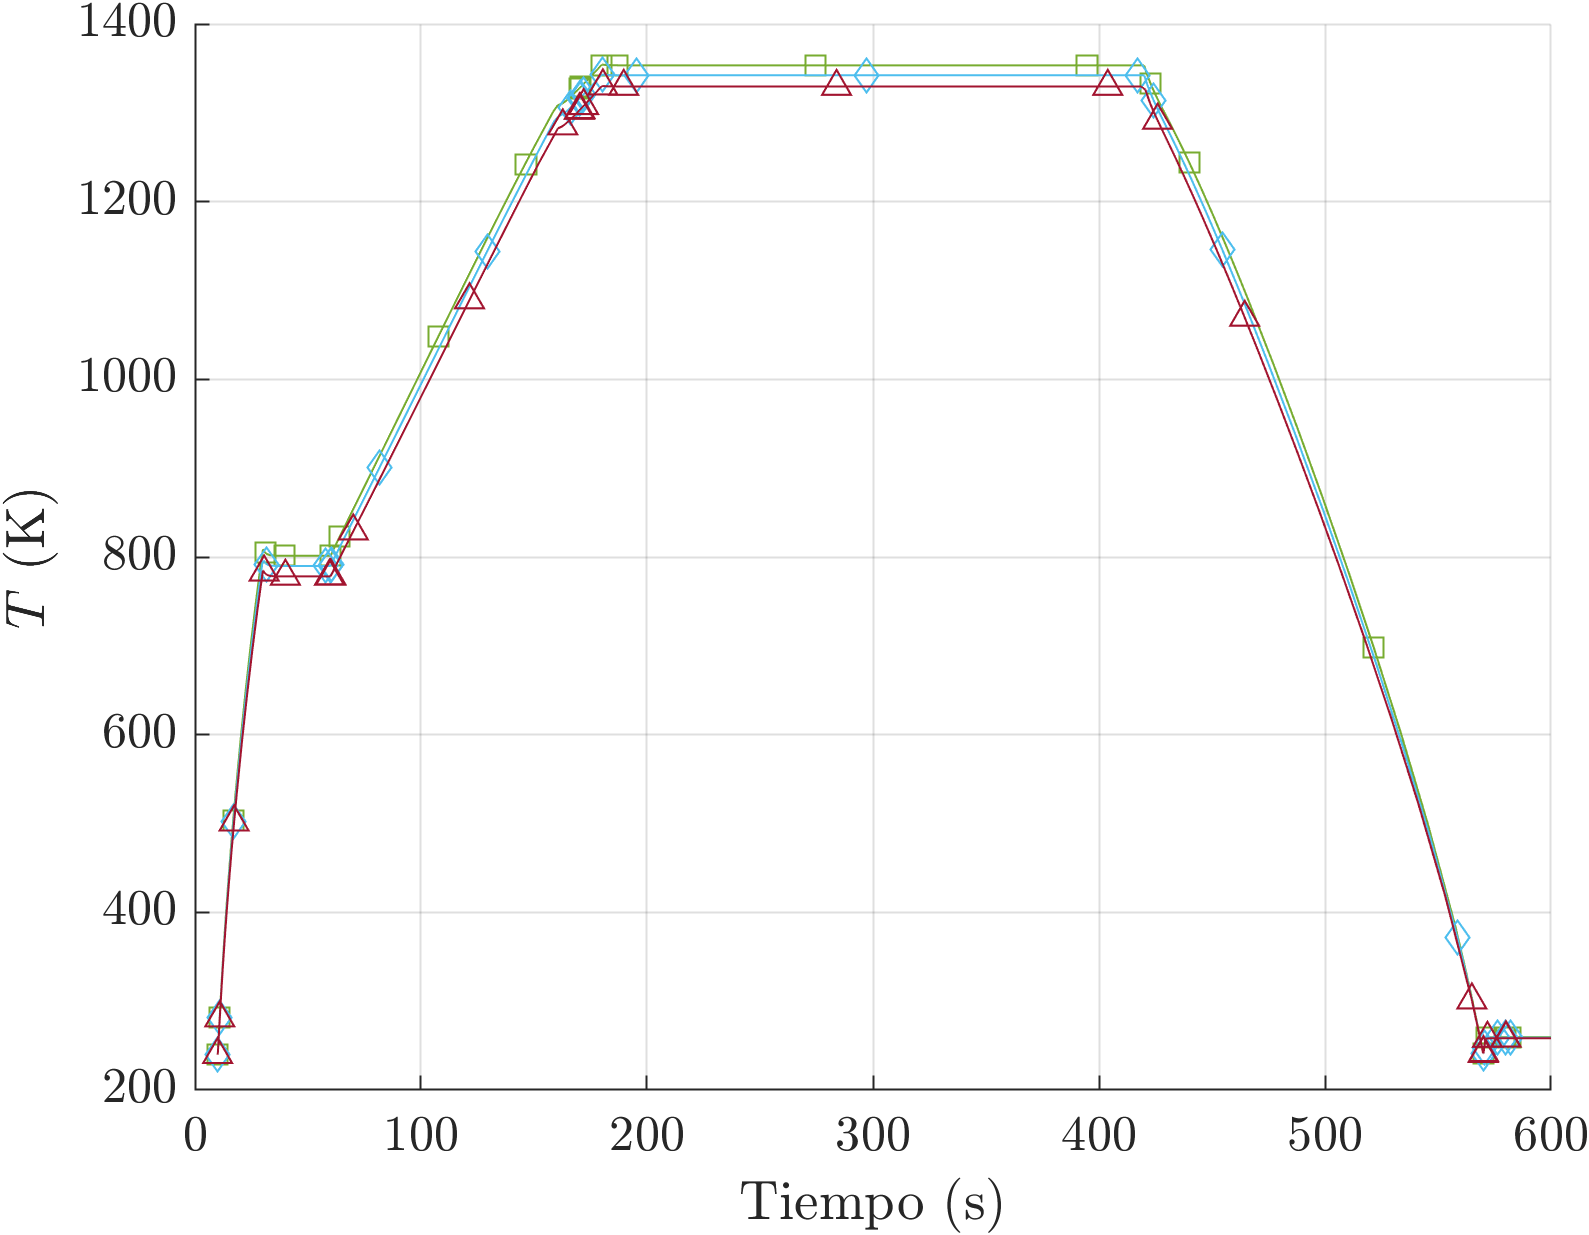
\includegraphics[width=\textwidth]{grafica_T_turb_combustibles.png}
        \caption{Turbine stage temperature}
        \label{fig:T_turb_turbo}
    \end{minipage}
\end{figure}

Concerning thrust shown in \autoref{fig:thrust_T}, the observations were consistent with those from the pressure analysis: the inability of the blends to efficiently transfer thermal energy into mechanical energy allowed Jet A1 to maintain a clear performance advantage. During the cruise phase, the recorded thrust values were approximately 2300 N for Jet A1, 2000 N for the 75/25 blend, and 1800 N for the 50/50 blend. This analysis reinforces the superior performance of Jet A1, particularly in phases requiring sustained energy conversion efficiency.

% segunda fila: Gráfico individual del ángulo de paso 
\begin{figure}[H]
\centering
    \begin{minipage}{0.45\textwidth}
        \centering
        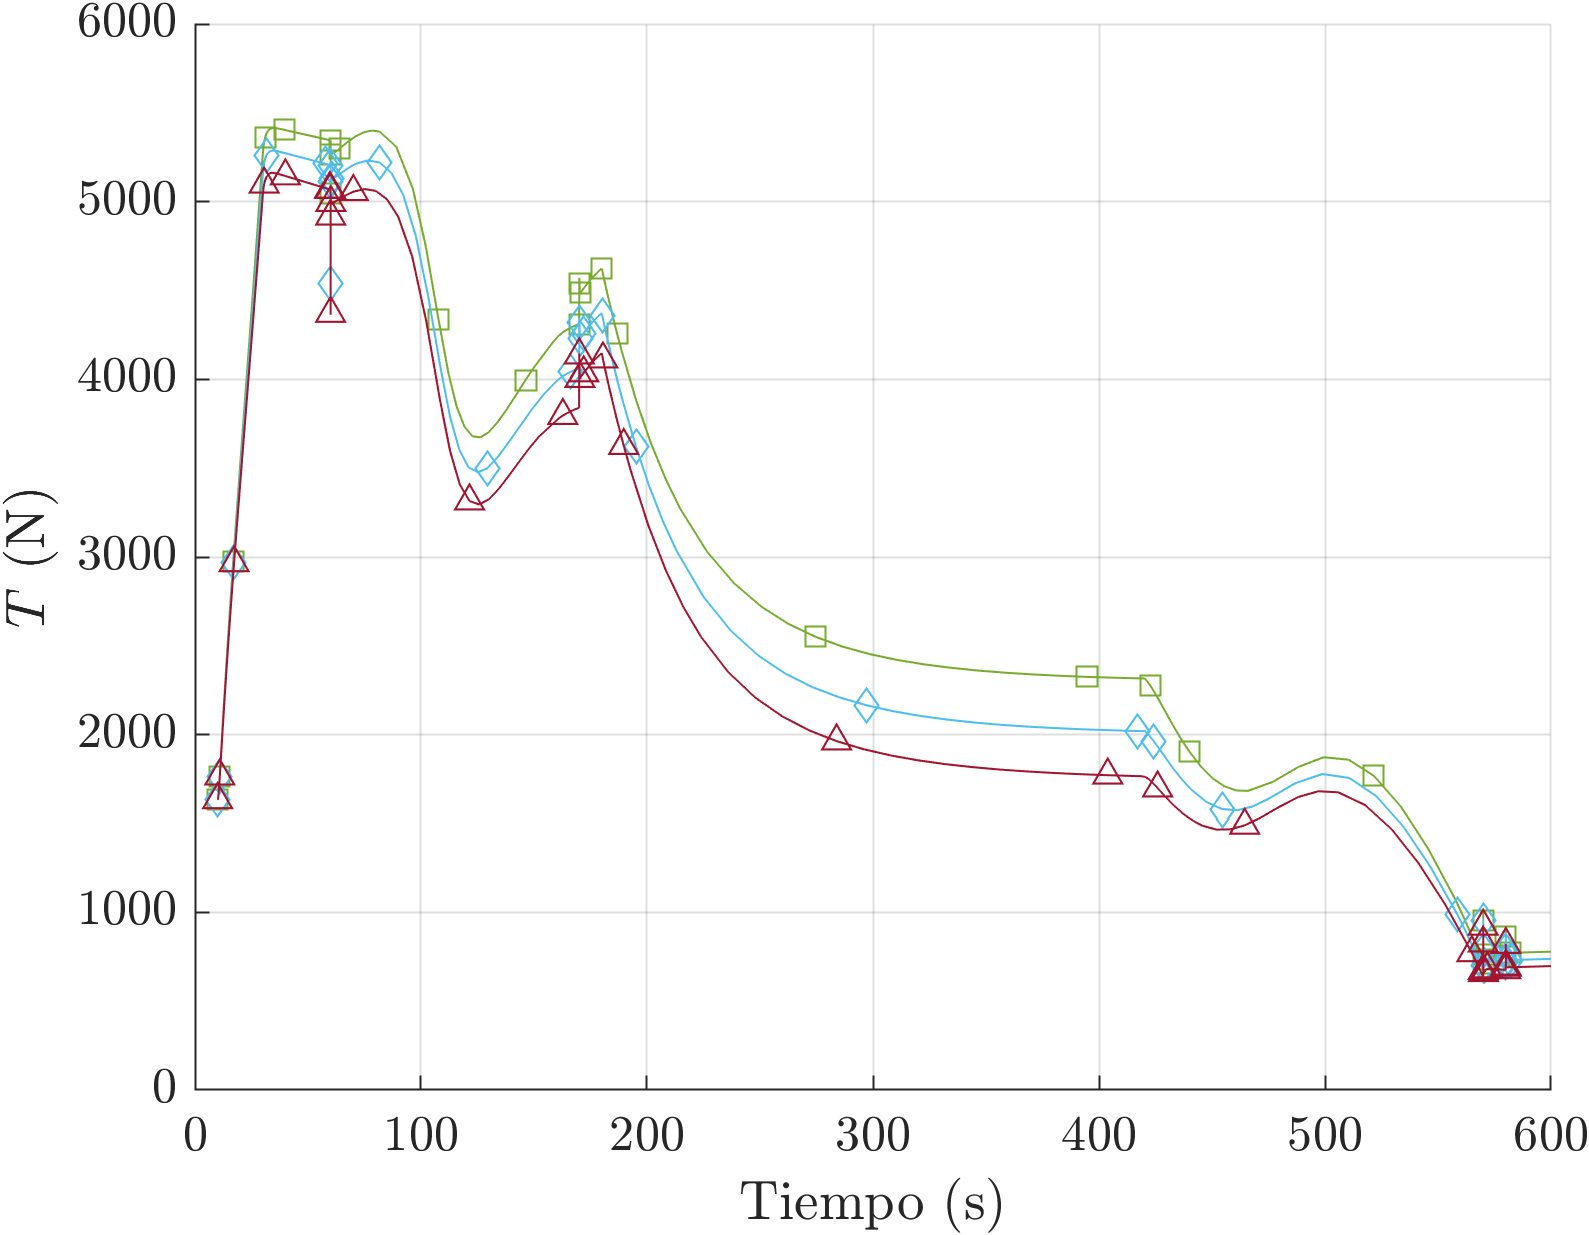
\includegraphics[width=\textwidth]{grafica_T_combustibles.png}
        \caption{Thrust $T$}
        \label{fig:thrust_T}
    \end{minipage}
\end{figure}

The propulsive efficiencies (\autoref{fig:propulsive_efficiency}) reflected the trends observed in thrust values from \autoref{fig:Turboprop_Efficiency_Pitch Angle}, \cite{A1specs2018} and \cite{Mehta2009LHV}. Jet A1 demonstrated the highest efficiency among the studied fuels, with efficiency decreasing as the concentration of Jet A1 in the blends decreased. It should be noted that the efficiency values are constrained by simulator limitations, as discussed in Chapter 3, due to low advance ratio (\( J \)) values. Nevertheless, these results provide a preliminary insight into potential performance at higher speeds. A notable aspect is the convergence of the efficiencies of all three fuels to approximately 30\% at around 200 seconds of simulation. This behavior is partially attributable to the limited speeds, which do not allow for a comprehensive view of performance under optimal conditions.

\begin{equation}\label{eq:Propulsion_Tuboprop_Efficiency_PULIDO}
    \eta_{P} = 1 - \frac{T_{4}-T_{1}}{T_{3}-T_{2}}
\end{equation}

\vspace{50pt}
Finally, thermal efficiencies shown in \autoref{fig:thermal_efficiency} were related to temperature values, \cite{pulido2008conversión} explains another way to calculate thermal efficiency relating turbines temperature values as in equation \eqref{eq:Propulsion_Tuboprop_Efficiency_PULIDO}, this means closely temperature values in \autoref{fig:T_turb_turbo} will show similar efficiencies. Since the temperatures showed no significant differences between the blends, the thermal efficiencies also remained within a consistent range, with values not falling below 30\%. However, upon closer inspection, a slight separation in efficiency values was evident, further highlighting the dominance of pure Jet A1 over the proposed blends due to its superior energy conversion capacity.
% tercera fila: Eficiencias n_prop y n_termal

\begin{figure}[H]
\centering
    \begin{minipage}{0.45\textwidth}
        \centering
        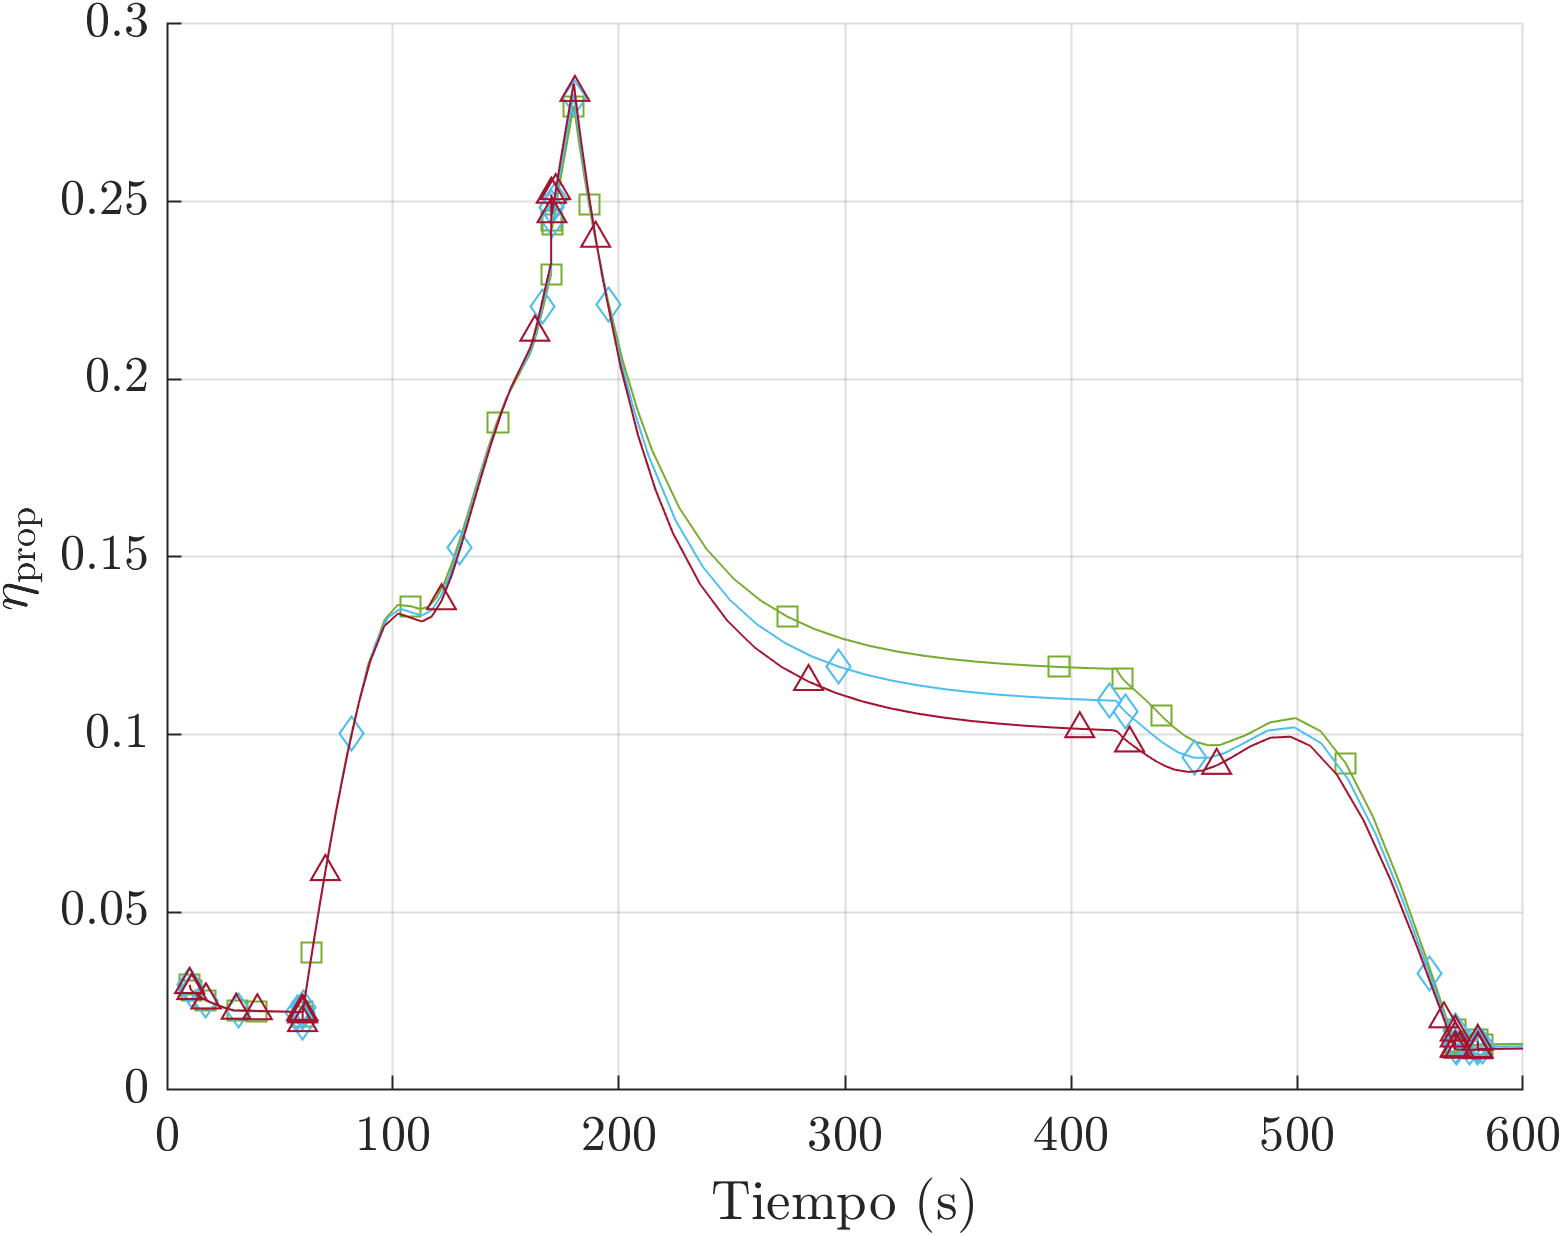
\includegraphics[width=\textwidth]{grafica_n_prop_combustibles.png}
        \caption{Propulsive efficiency $\eta_{prop}$}
        \label{fig:propulsive_efficiency}
    \end{minipage}
    \hfill
    \begin{minipage}{0.45\textwidth}
        \centering
        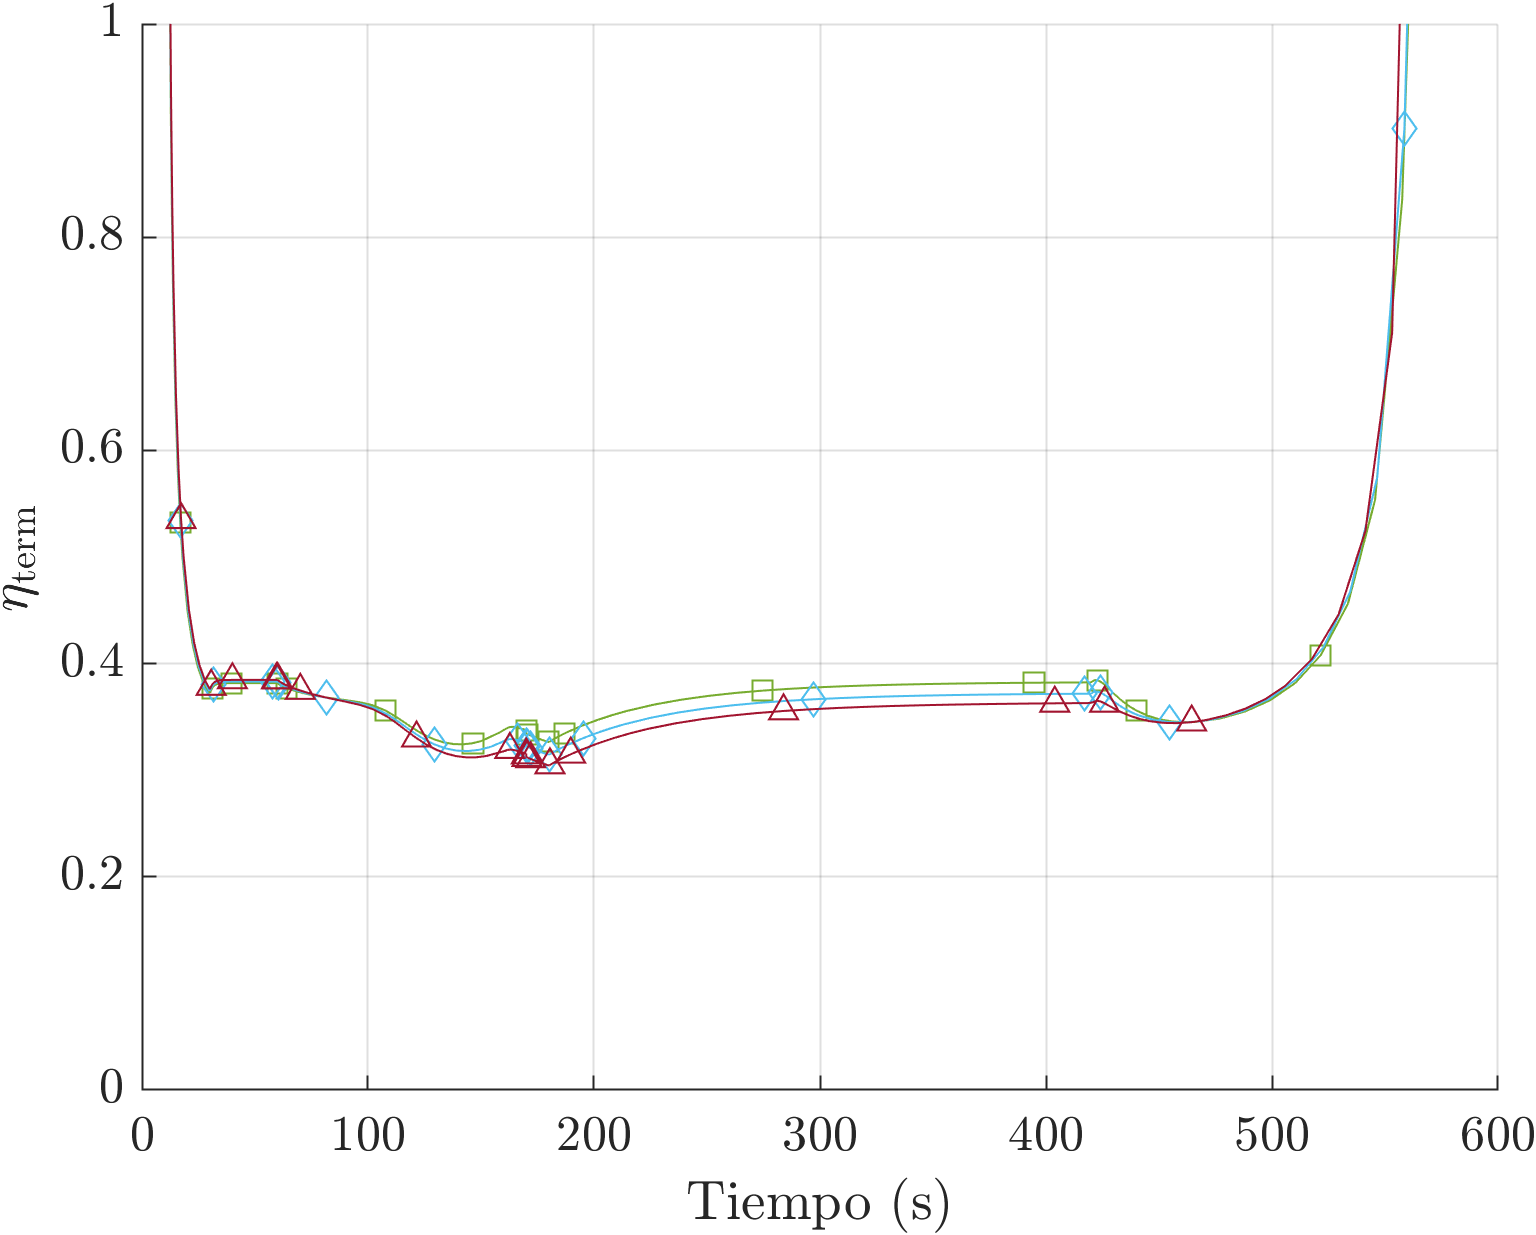
\includegraphics[width=\textwidth]{grafica_n_term_combustibles.png}
        \caption{Thermal efficiency $\eta_{th}$}
        \label{fig:thermal_efficiency}
    \end{minipage}
\end{figure}

\section{Conclusions}
A Simulink model was developed to effectively integrate the two primary components of a turboprop engine: the PT6A engine and the McCauley propeller. This structure provides an optimal and accessible framework for simulating the various conditions and phenomena encountered by this dynamic system during flight. The Matlab-Simulink-based tool effectively captures the key parameters, such as RPM, temperature, pressure, and torque, required for a comprehensive analysis of the turboprop's performance during a simulated flight from El Dorado Airport to Guaymaral Aerodrome.

Upon validating the model against manuals and references from the state of the art, several findings were identified. For the engine model, the results were compared with reference values from the PT6 manual, yielding errors of 6.73\% for compressor pressure, 1.05\% for combustion chamber temperature, and 4.95\% for gas generator shaft speed. This confirms that the implemented model reliably represents the engine phenomena, though with certain limitations, such as the exclusion of heat losses and the fact that not all the fuel burns completely in real-life scenarios.

By propeller validation, it was observed that the revolutions did not exceed the established 2200 rpm limit as indicated in \cite{Piper1998}, and remained within the desired range throughout the various flight phases. Additionally, torque and thrust showed a consistent response to pitch angle adjustments, as anticipated in \cite{Castellanos2023Propeller}, with increases aligning closely with changes in pitch.

Finally, during complete turboprop system validation, the obtained results demonstrated the precision of this computational tool. The PID controller adjusted the pitch angle as expected, within a range of 22° to 84.5°, as specified in \cite{Castellanos2023Propeller}; the engine, meanwhile, operated within safe temperature limits and displayed an error of up to 10\%, while the pressure exhibited a 16\% error compared to reference values in \cite{Castellanos2019}. The propeller RPM remained below maximum 2200 RPM limit, indicating strong performance in terms of both torque and thrust, with torque remaining below the operational threshold of 3086 Nm. Furthermore, the shaft speeds met expected values from \cite{Piper1998}, with 45,000 RPM for the gas generator shaft and 30,000 RPM for the power generation shaft.

An important aspect to highlight about the developed model is its maximum speed limit for accurate predictions and consistency with reference parameters, which is 60 m/s. After conducting multiple simulations across a wide range of speeds, it was determined that the model maintains applicability only up to this maximum speed, making it suitable for a specific group of aircraft operating at or below this threshold, such as \cite{cessna_skyhawk_2024}, Piper PA-28 Cherokee \cite{piper_cherokee_2021}, and Diamond DA-20 \cite{diamond_da20_2024}, named previously. Further details on these limitations are discussed in the following section.

Finally, to achieve a comprehensive assessment of the engine and propeller performance, thermal and propulsive efficiencies were determined, respectively. The thermal efficiency in the developed model reached a value of 40\%, aligning with the analysis presented in \cite{pulido2008conversión}. Additionally, the propulsive efficiency reached 27\%, which is consistent with values reported in \cite{book:96630002} for aircraft at similar speeds. This result is logical, considering that, as previously mentioned, the maximum achievable speed in the model was 60 m/s, resulting in a lower advance ratio compared to other aircraft.
\vspace{5pt}

In conclusion, the results obtained from the Jet A1 and biodiesel blends demonstrate that, although the blends exhibit relatively stable thermal behavior, Jet A1 maintains a clear advantage in terms of mechanical performance and efficiency. In the pressure analysis, the blends remained below the operational limit of 730 kPa, with the 50/50 blend showing an 18\% reduction in torque compared to Jet A1, particularly during the cruise phase. Regarding temperature, the differences were minimal, with a maximum deviation of 35 K, suggesting similar thermal stability across the fuels. However, thrust values revealed a more significant difference, with Jet A1 reaching a thrust of 2300 N during the cruise phase, while the 75/25 blend reached 2000 N and the 50/50 blend reached 1800 N. Propulsive and thermal efficiencies showed a similar trend, with Jet A1 demonstrating the highest efficiency, around 30\%, while the blends exhibited slight reductions in efficiency, further confirming Jet A1’s superiority due to its better energy conversion capacity.

\section{Limitations and Recomendations}

During the development of the model, various limitations were identified that affected accuracy and applicability under certain conditions. First, the simulation reached a maximum speed of 60 m/s; attempting to exceed this limit resulted in incoherent values in critical variables, such as torque, which showed negative values, as well as thrust, propeller RPM, and pitch angle, which exceeded permitted limits. These results suggest that the model did not optimally adapt to higher speeds, impacting the reliability of results under these conditions. Additionally, the model employs a simplified approach to handling thermodynamic parameters, omitting potential alterations due to temperature and/or pressure gradients, where these can significantly influence engine performance and limit the model’s ability to accurately represent these variations under real operating conditions. Furthermore, the governor’s simulation was simplified using a PID control system instead of a dynamic mechanical-hydraulic system, which would better represent the actual function of the governor in the engine, suggesting an opportunity for improvement in future studies. Additionally, it was noted that the simplification of the combustion modeling within the chamber does not fully reflect the chemical reactions, generating power values higher than the real ones, which impacts accuracy in predicting engine performance.

Despite these limitations, the simulation performed optimally in treating thermodynamic variables, densities, and viscosities, which varied with altitude under the international atmosphere model. However, as the aircraft’s speed increased, the Traub methodology together with the PID system showed limitations, resulting in inconsistent values and errors that increased proportionally with speed, reaching errors of 100\% under high-speed conditions. This sensitivity suggests the need for adjustments or alternative methods in this operating range. In general, the model maintained acceptable accuracy under limited-speed conditions, with errors in key variables not exceeding the range of 5 to 10\%. This accuracy, within the established speed limitations, supports the model’s utility for simulations at moderate speeds, although it highlights the need for review and adaptation for higher speeds.

Based on these observations, several recommendations are suggested for future research. First, implementing a real-time model using advanced control libraries in Simulink could optimize variable management and reduce the dependence on assumptions. This approach would allow a more accurate representation of the engine’s dynamic conditions. Additionally, expanding the analysis to include the aircraft’s complete aerodynamics would help better understand loads on the engine, especially at high-speed conditions, and would contribute to obtaining more precise results by better reflecting interactions between the engine and the aircraft’s aerodynamic environment. Another recommendation is to explore other calculation models for aerodynamic analysis, such as CFD (Computational Fluid Dynamics), aiming to improve accuracy by incorporating compressibility effects in the Navier-Stokes equations. Similarly, a change in the BEMT Traub model to other already-developed derivations or new models could yield results that improve upon those found in this study through innovative correction factors or algorithms. Finally, performing an analysis from the temperature-entropy perspective could facilitate the tracking of certain engine variables and allow a complete evaluation of thermodynamic behavior, providing a solid foundation to improve performance prediction under various operating conditions.

Regarding the tools used, XFOIL presented limitations in the ranges of attack angles employed, which did not fully cover the propeller’s design ranges. For future simulations, it would be advisable to complement/replace the Panel Method-based (XFOIL) with other software such as VLM (Vortex Lattice Method) or RAMS (Rotor Aerodynamics and Modeling Software) through CAD/CAE interfaces (e.g. Ansys) or in libraries for Python or MATLAB code, which would allow for result comparisons and improved accuracy. As for Simulink, although it met the proposed objectives, its complexity and high-level programming suggest that good proficiency in the interface is essential for adjusting the model in future studies.



\newpage

\bibliography{References}

\end{document}
